\documentclass[12pt, a4paper, twoside]{article}

\usepackage[brazilian]{babel}
\usepackage[utf8]{inputenc}
\usepackage[top = 3cm, left = 3cm, bottom = 2cm, right = 2cm]{geometry}

\usepackage{graphicx} % Possibilita inclusão de imagem
\usepackage{tikz} % Permite desenhar
\usepackage{pgfplots} % Com tikz, desenha gráfico
\usetikzlibrary{patterns} % Permite hachurar áreas
\usetikzlibrary{decorations.pathreplacing, angles, quotes} % Permite desenhar "chaves"
\usepackage{mathtools, amsthm, amssymb, amsbsy} % Pacotes de Matemática
\usepackage[makeroom]{cancel}
\usepackage{indentfirst} % Identa o primeiro parágrafo de cada seção
\usepackage{changepage} % Permite mudar as margens para um bloco de texto
\usepackage{afterpage} % Permite incluir página em branco
\usepackage[numbers]{natbib} % Configuração de Referências
\usepackage{titlesec} % Permite iniciar cada subseção em uma nova página 
\usepackage{titleps} % Permite customização do cabeçalho e rodapé (ORDEM IMPORTA: depois do 'titlesec')
\usepackage{colonequals} % Símbolo de definição: \colonequals ou \equalscolon
\usepackage{hyperref} % Link para partes do próprio texto
\usepackage[shortlabels]{enumitem} % Permite trocar a numeração da lista
\usepackage{pdfpages}
\allowdisplaybreaks

% DEIXAR O CARREGAMENTO DE hyperref POR ÚLTIMO
\usepackage{color}   % May be necessary if you want to color links
\usepackage{hyperref}
\hypersetup{
	colorlinks = true,  % Set true if you want colored links
	allcolors  = black
}

% DEFINIÇÃO DE ESPAÇAMENTO
\setlength{\parindent}{1.25cm}
\setlength{\parskip}{0pt}
\renewcommand{\baselinestretch}{1.5}

% TIRA TÍTULO AUTOMÁTICO DA SEÇÃO DE SUMÁRIO
\makeatletter
\renewcommand\tableofcontents{%
	\@starttoc{toc}%
}
\makeatother

% TIRA TÍTULO AUTOMÁTICO DA SEÇÃO DE REFERÊNCIAS
\renewcommand{\bibsection}{}

% INICIA CADA SEÇÃO EM UMA NOVA PÁGINA
\newcommand{\sectionbreak}{\clearpage\thispagestyle{plain}}

% PERMITE INCLUIR NUMERAÇÃO EM APENAS UMA EQUAÇÃO DO ALIGN*
\newcommand\numberthis{\addtocounter{equation}{1}\tag{\theequation}}

% DEFINIÇÃO DE NOVOS SÍMBOLOS
\DeclareMathOperator{\PX}{\mathbb{P}} % Probability symbol
\DeclareMathOperator{\EX}{\mathbb{E}} % Expectation symbol \mathbbmss
\DeclareMathOperator{\VX}{\mathbb{V}} % Variance symbol
\DeclareMathOperator{\FX}{\mathcal{F}} % Sigma-algebra symbol
\DeclareMathOperator{\AX}{\mathcal{A}} % Sigma-algebra symbol
\DeclareMathOperator{\NX}{\mathbb{N}} % Natural set symbol
\DeclareMathOperator{\ZX}{\mathbb{Z}} % Integer set symbol
\DeclareMathOperator{\QX}{\mathbb{Q}} % Rational set symbol
\DeclareMathOperator{\IX}{\mathbb{I}} % Irrational set symbol
\DeclareMathOperator{\RX}{\mathbb{R}} % Real set symbol
\DeclareMathOperator{\CX}{\mathbb{C}} % Complex set symbol
\DeclareMathOperator{\LX}{\mathbb{L}} % Lattice set symbol
\DeclareMathOperator{\GX}{\mathcal{G}} % Group symbol
\DeclareMathOperator{\VL}{\mathcal{V}} % 
\DeclareMathOperator{\HL}{\mathcal{H}} % 
\newcommand{\diff}{{\nabla_i}f(\omega)}
\newcommand{\flip}{\text{Flip}_i(\omega)}
\newcommand{\infl}{\text{Inf}_i(f(\omega))}
\newcommand{\diffe}{{\nabla_e}f(\omega)}
\newcommand{\infle}{\text{Inf}_e(f(\omega))}
\newcommand{\flipe}{\text{Flip}_e(\omega)}

% DEFINIÇÃO DE TEOREMAS, LEMAS, ETC. (+ SÍMBOLO DE DEMONSTRAÇÃO)
\theoremstyle{definition} % Define padrão de formatação - default: plain
\newtheorem{mydef}{Definição}[section]
\newtheorem{mythm}{Teorema}[section]
\newtheorem{mylem}{Lema}[section]
\newtheorem{mypro}{Proposição}[section]
\newtheorem{mycol}{Corolário}[section]
\newtheorem{mynot}{Nota}[section]
\newtheorem{myexp}{Exemplo}[section]

\definecolor{darkgreen}{rgb}{0.0, 0.2, 0.0}

\newpagestyle{main}{%
	\setheadrule{1pt}%
	\sethead[\thesection~\sectiontitle][][] % Par
			{}{}{\thesubsection~\subsectiontitle} % Ímpar
	\setfoot[][\thepage][]%
			{}{\thepage}{}
}

\makeatletter % DEFINE A FUNÇÃO 'ERF'
\pgfmathdeclarefunction{erf}{1}{%
	\begingroup
	\pgfmathparse{#1 > 0 ? 1 : -1}%
	\edef\sign{\pgfmathresult}%
	\pgfmathparse{abs(#1)}%
	\edef\x{\pgfmathresult}%
	\pgfmathparse{1/(1+0.3275911*\x)}%
	\edef\t{\pgfmathresult}%
	\pgfmathparse{%
		1 - (((((1.061405429*\t -1.453152027)*\t) + 1.421413741)*\t 
		-0.284496736)*\t + 0.254829592)*\t*exp(-(\x*\x))}%
	\edef\y{\pgfmathresult}%
	\pgfmathparse{(\sign)*\y}%
	\pgfmath@smuggleone\pgfmathresult%
	\endgroup
}
\makeatother

\begin{document}
	
	% Elementos pré-textuais
	
	\newpage

\begin{center}
	{\normalsize UNIVERSIDADE FEDERAL DE MINAS GERAIS} \\
	{\normalsize INSTITUTO DE CIÊNCIAS EXATAS} \\
	{\normalsize DEPARTAMENTO DE ESTATÍTICA} \\ \vspace{6cm}
	{\LARGE Transição de Fase em Modelos de Percolação via Funções Booleanas} \\ \vspace{4.4cm}
	{\Large André Victor Ribeiro Amaral} \\ \vspace{0.75cm}
	{\large Orientador: Roger William Câmara Silva.} \\ \vspace{7cm}
	{\normalsize Belo Horizonte} \\
	{\normalsize 2020}
\end{center}

\thispagestyle{empty} \newpage

\begin{center}
	\vspace*{\fill}
	{\normalsize \phantom{Texto em branco.}}
	\vspace*{\fill}
\end{center}

\thispagestyle{empty}
	\newpage

\begin{center}
	{\Large André Victor Ribeiro Amaral} \\ \vspace{7.5cm}
	{\LARGE Transição de Fase em Modelos de Percolação via Funções Booleanas} \\ \vspace{3.2cm}
	\begin{adjustwidth}{8cm}{0cm}
		{\normalsize Dissertação submetida ao Programa de Pós-Graduação em Estatística da Universidade Federal de Minas Gerais, como requisito parcial para obtenção do título de Mestre em Estatística. \\
		Orientador: Roger William Câmara Silva.}
	\end{adjustwidth} \vspace{5.7cm}
	{\normalsize Belo Horizonte} \\
	{\normalsize 2020}
\end{center}

\thispagestyle{empty}
	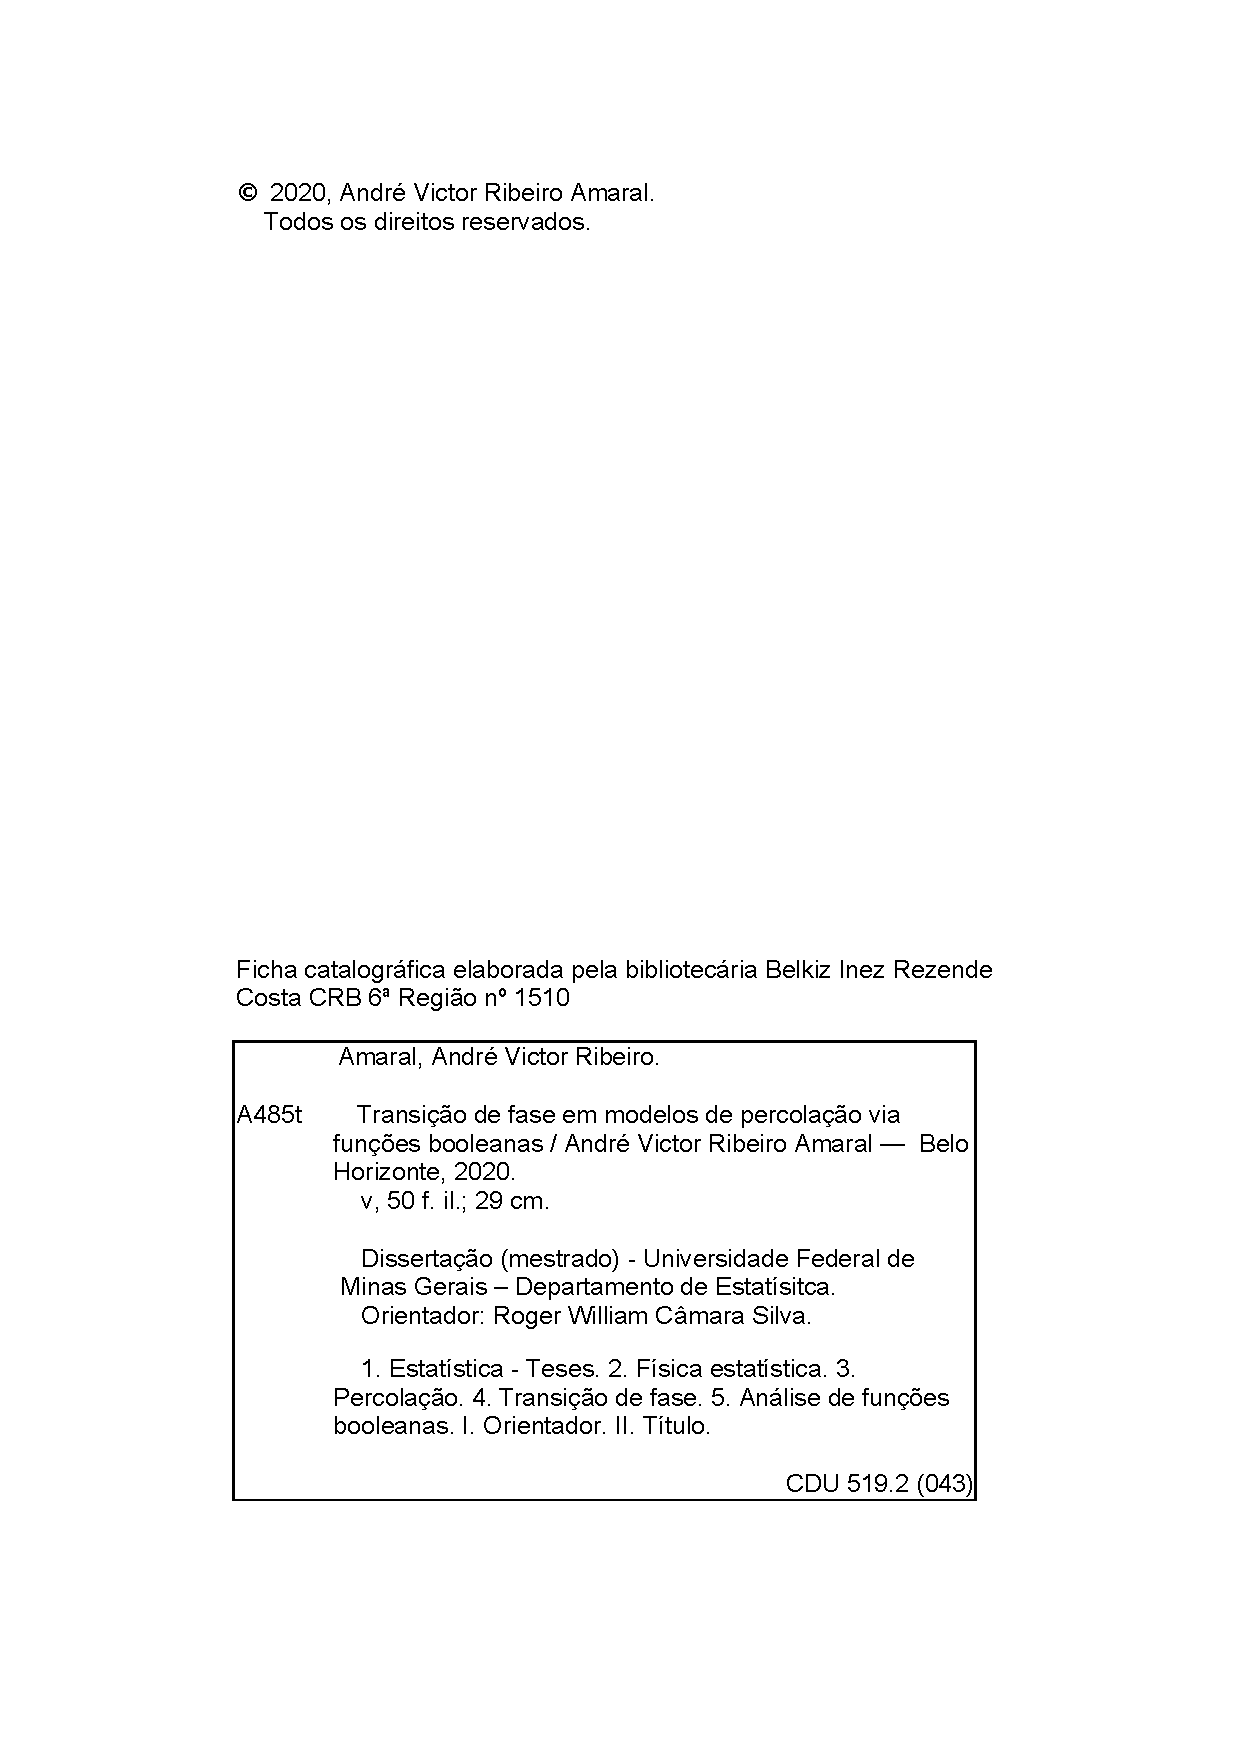
\includepdf{ficha-catalografica.pdf}
	%\newpage

\begin{center}
	\vspace*{\fill}
	{\normalsize Incluir \textit{ficha catalográfica}.}
	\vspace*{\fill}
\end{center}

\thispagestyle{empty}
	%\newpage

\begin{center}
	\vspace*{\fill}
	{\normalsize Incluir \textit{ata de defesa}.}
	\vspace*{\fill}
\end{center}

\thispagestyle{empty}
	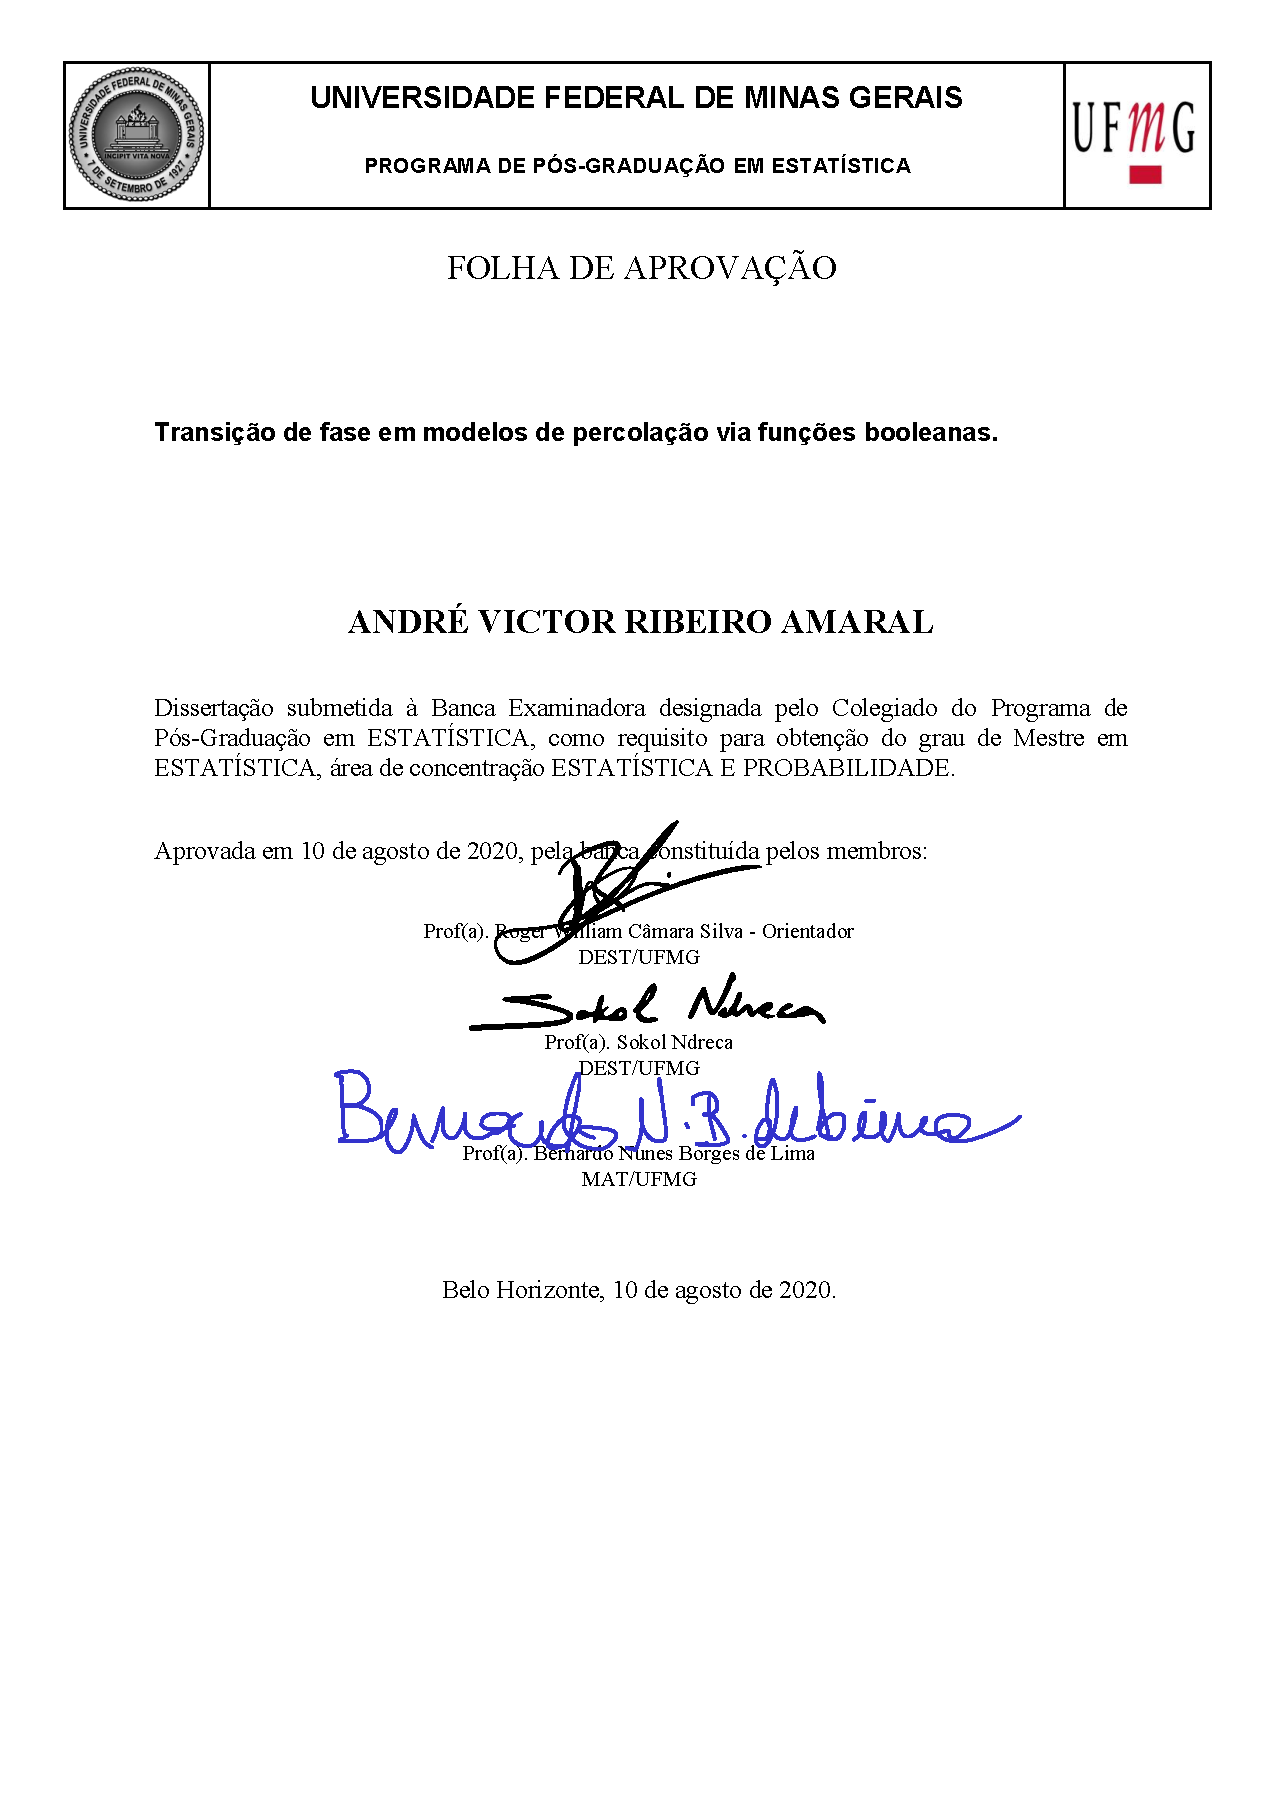
\includepdf{folha-de-aprovacao.pdf} \newpage

\begin{center}
	\vspace*{\fill}
	{\normalsize \phantom{Texto em branco.}}
	\vspace*{\fill}
\end{center}

\thispagestyle{empty}
			
	\newpage

\phantomsection
\section*{\Large \hspace*{\fill} \textbf{Agradecimentos} \hspace*{\fill}}
\addcontentsline{toc}{section}{Agradecimentos}

À minha \textit{mãe} (Alexandra) e \textit{irmã} (Melissa), o meu agradecimento mais do que especial. O suporte de vocês sempre será de fundamental importância.

Ao Professor Roger William Câmara Silva, obrigado pela orientação, pela paciência, e por contribuir de maneira tão positiva na minha (ainda em construção) formação acadêmica.

Aos colegas que fiz na UFMG, em especial aos companheiros de estudo Otávio e (por um período mais curto de tempo) Matheus, o meu ``muito obrigado''. 

Finalmente, um agradecimento à CAPES pelo suporte financeiro oferecido para o desenvolvimento deste trabalho.
	
	\pagenumbering{Roman} \newpage

\begin{center}
	\vspace*{\fill}
	{\normalsize Esta página foi \textit{intencionalmente} deixada em branco.}
	\vspace*{\fill}
\end{center}


	
	\newpage

\phantomsection
\section*{\Large \hspace*{\fill} \textbf{Resumo} \hspace*{\fill}}
\addcontentsline{toc}{section}{Resumo}

O conceito de \textit{transição de fase}, inerente a diferentes tipos de modelos puramente determinísticos, pode, também, ser verificado em sistemas com componentes estocásticas. Nesse sentido, é importante o estudo de ferramentas que nos permitem provar que determinados sistemas aleatórios apresentam esse tipo de característica. 

Assim, dado um espaço de probabilidade apropriado, resultados associados à análise de funções Booleanas desempenham papel importante no estudo dessa classe de modelos. Este texto preocupa-se em, ao longo da Seção \ref{How-to-prove}, apresentar e demonstrar tais resultados.

Tratando-se de modelos aleatórios independentes e que vêm da Física Estatística, o de Percolação Bernoulli é, talvez, o mais conhecido. Por isso, na Seção \ref{Bernoulli-percolation}, nos concentramos em reproduzir alguns resultados ``clássicos'' desse modelo; utilizando, porém, as ferramentas desenvolvidas na Seção \ref{How-to-prove}. Aqui, é importante ressaltar o ganho que existe em utilizar esse tipo de abordagem. Alguns dos resultados demonstrados poderão ser estendidos, utilizando-se de estratégias similares, para modelos construídos sobre espaços mais gerais $-$ incluindo modelos com dependência, como os que foram discutidos na Seção \ref{Monotonic-measures}.

Por fim, deixo o registro de que os resultados apresentados ao longo desse texto \textbf{não} são originais. O trabalho foi construído a partir de, principalmente, \cite{duminil2019sharp} $-$ em adição aos outros artigos e recursos que foram apropriadamente referenciados.

\vspace{12pt}

\par Palavras-chave: transição de fase; \textit{sharp threshold}; análise de funções Booleanas; percolação.

	\newpage

\phantomsection
\section*{\Large \hspace*{\fill} \textbf{Abstract} \hspace*{\fill}}
\addcontentsline{toc}{section}{Abstract}

The \textit{phase transition} concept, intrinsic to some purely deterministic models, may also be seen in systems with some stochastic component. Therefore, it is important to study results that allow us to prove that some arbitrary random systems present such a characteristic.

In this regard, given an appropriate probability space, results associated with Boolean function analysis play an important role in the study of this class of models. As a consequence of it, this text focuses on, throughout Section \ref{How-to-prove}, introduce and prove such results. 

With respect to independent random models from Statistical Physics, the Bernoulli Percolation Model may be considered the most popular one. Thus, in Section \ref{Bernoulli-percolation}, we focused on replicating some ``classical'' results concerned with it. In order to achieve this, we used the tools developed in Section \ref{How-to-prove}. At this point, it is important to stress the benefits of adopting such an approach. Some of the proofs may be extended, through similar strategies, to models defined over more general spaces $-$ which also includes models with a structure of dependence, as discussed in Section \ref{Monotonic-measures}.

Finally, I would like to clarify that the results presented throughout this text are \textbf{not} original. This work was developed mainly based on \cite{duminil2019sharp} $-$ in addition to other resources and academic articles, which were properly cited.

\vspace{12pt}
\par Keywords: phase transition; sharp threshold; Boolean functions analysis; percolation.
 
		
	\newpage

\begin{center}{\Large \textbf{Sumário}}\end{center}
	
\tableofcontents

\thispagestyle{empty} \newpage

\begin{center}
	\vspace*{\fill}
	{\normalsize \phantom{Texto em branco.}}
	\vspace*{\fill}
\end{center}

\thispagestyle{empty}
	
	% Elementos textuais
		
	\newpage
\pagestyle{main}

\section{Introdução}\label{Intoduction} \vspace{24pt} \pagenumbering{arabic}

\par Na física, \textit{transição de fase} pode ser caracterizada como a mudança descontínua do estado físico de um sistema à medida que algum de seus parâmetros varia continuamente. O exemplo mais simples vem, talvez, da mudança do estado físico da matéria: sólido, líquido ou gasoso $-$ dependendo de parâmetros como temperatura e pressão.

\par Tratando-se, porém, de modelos com componentes estocásticas, dizemos que um sistema aleatório finito passa por \textit{sharp threshold} se o seu comportamento muda rapidamente como resultado de uma pequena perturbação dos parâmetros que governam sua estrutura. O modelo de percolação Bernoulli, que será formalmente enunciado na Seção \ref{Bernoulli-percolation}, é um dos principais exemplos que vamos estudar ao longo deste texto.

\par O modelo probabilístico assumido, a menos que seja dito o contrário, será descrito pelo espaço de probabilidade $(\Omega_n, \AX, \QX_p)$, tal que $\Omega_n = \{0,1\}^n$ com $\omega = (\omega_1, \cdots, \omega_n) \in \Omega_n$ e $n \in \NX$, $\AX = \mathcal{P}(\Omega_n)$, onde $\mathcal{P}(\cdot)$ é o conjunto das partes, e $\QX_p(\omega) = \prod_{i:\omega_i = 1} p \prod_{i:\omega_i = 0} (1 - p)$ é a medida produto Bernoulli com parâmetro $p$. A fim de simplificar notação, denote o conjunto $\{1, \cdots, n\}$ por $[n]$ .

\par Dentro do espaço de probabilidade apresentado, este texto se concentrará em estudar funções do tipo $f: \Omega_n \longrightarrow \{0,1\}$, chamadas de \textit{funções Booleanas}. Assim, defina $F(p) \colonequals \EX_p(f(\omega))$, onde $\EX_p(\cdot)$ é \textit{valor esperado} com respeito à medida $\QX_p$. Da mesma forma, defina $F_n(p) \colonequals \EX_p(f_n(\omega))$ para uma sequência de funções $(f_n)_{n \in \NX}$ tal que $f_n: \Omega_n \longrightarrow \{0,1\}$, $\forall n \in \NX$. Por fim, note que, como $\QX_p$ é medida produto Bernoulli,
\begin{align}\label{eq-esperanca}
	F_n(p) = \sum_{\omega \in \Omega_n} f_n(\omega) \; p^{\sum_{i \in [n]}\omega_i} \; (1 - p)^{\sum_{i \in [n]}1 - \omega_i}\text{, }\forall n \in \NX.
\end{align} 
\par Em adição, dadas duas configurações $\omega, \omega' \in \Omega_n$, dizemos que $\omega \leq \omega'$ se $\omega_i \leq \omega'_i$, $\forall i \in [n]$ $-$ nesse caso, foi determinada uma ordem parcial para os elementos do espaço amostral $\Omega_n$. Assim, $f(\omega)$ é dita \textit{crescente} se $f(\omega) \leq f(\omega')$ sempre que $\omega \leq \omega'$. Estabelecidas as quantidades de interesse, a definição a seguir irá formalizar a ideia de \textit{sharp threshold}.

\begin{mydef}\label{sharp-threshold}
	Uma sequência de funções Booleanas crescentes $(f_n)_{n \in \NX}$ passa por \textit{sharp threshold} em $(p_n)_{n \in \NX}$ se existe $(\delta_n)_{n \in \NX}$, com $\delta_n > 0$, $\forall n \in \NX$, e $\lim_{n \rightarrow +\infty} \delta_n = 0$, tal que $F_n(p_n - \delta_n) \longrightarrow 0$ e $F_n(p_n + \delta_n) \longrightarrow 1$, quando $n \rightarrow +\infty$.
\end{mydef}

\par Perceba que, da Definição \ref{sharp-threshold}, é possível ver que, se $f_n(\omega) = \IX_{A_n}(\omega)$, onde $\IX_{A_n}(\omega)$ é função indicadora de $\omega$ em $A_n \in \AX$, então $F_n(p) = \EX_p(f_n(\omega)) = \EX_p(\IX_{A_n}(\omega)) = \QX_p(A_n)$, $\forall n \in \NX$. Isto é, se $(f_n)_{n \in \NX}$ passa por \textit{sharp threshold}, então para $n$ ``grande'' a medida $\QX_p(A_n)$ está, exceto na região $(p_n - \delta_n, p_n + \delta_n)$, perto de $0$ ou $1$; o que, de alguma forma, pode estar relacionado à \textit{transição de fase} (ou, \textit{transição de fase} ``\textit{afiada}'') pela qual o sistema que está sendo considerado é caracterizado. Abaixo, a Figura \ref{fig-sharp-threshold} apresenta um esboço esse fenômeno.

\begin{figure*}[!htbp]
	\centering
	\begin{tikzpicture}[scale = 0.9, declare function = {funcao(\x) = 0.5 + (0.5 * erf((ln(\x) - ln(1 - x))/(0.45254834)));}]
	\begin{axis}
	[
	name = myGraph,
	xmin = 0,
	xmax = 1.075,
	xtick = {0, 1},
	axis x line = bottom,
	ymin = 0,
	ymax = 1.075,
	ytick = {0,1},
	axis y line = middle,
	samples = 200,
	domain = 0:1,
	clip = false %
	]
	\addplot[blue, mark = none, thick] (x, {funcao(x)});
	\draw[densely dotted] (100, 0) -- (100, 100);
	\draw[densely dotted] (0, 100) -- (100, 100);
	\draw[densely dotted] (40,  0) -- (40,  100);
	\draw[densely dotted] (60,  0) -- (60,  100);
	\draw[densely dotted] (0,  10) -- (100,  10);
	\draw[densely dotted] (0,  90) -- (100,  90);
	\node[left] at (axis cs:0, 0.10) {\scriptsize{$F_n(p_n - \delta_n)$}};
	\node[left] at (axis cs:0, 0.90) {\scriptsize{$F_n(p_n + \delta_n)$}};
	\node[right] at (axis cs:1.075, 0) {\small{$p$}};
	\node[above] at (axis cs:0, 1.075) {\small{$F_n(p)$}};
	\draw[decoration = {brace, mirror, raise = 5pt}, decorate] (axis cs:0.4,0) -- node[below = 6pt] {{\scriptsize $2\delta_n$ }} (axis cs:0.6, 0);
	\end{axis}		
	\end{tikzpicture}
	%\vspace{-12pt}
	\caption{Esboço de $F_n(p) = \EX_p(f_n(w))$ para $n$ ``grande'', tal que $(f_n)_{n \in \NX}$ passa por \textit{sharp threshold}.} 
	\label{fig-sharp-threshold}
\end{figure*}

\par A seguir, com o propósito de indicar se as sequências de funções Booleanas $(f_n)_{n \in \NX}$ descritas passam (ou não) por \textit{sharp threshold}, dois exemplos serão apresentados.

\begin{myexp}\label{exemplo-1}
	Seja $f_n(\omega) = f(\omega) = \IX_{\{\omega_1 = 1\}}(\omega)$, $\forall n \in \NX$. Assim, o cálculo de $F_n(p) = F(p)$, $\forall n \in \NX$, utilizando a Expressão \eqref{eq-esperanca}, é dado por
	\begin{align*}
	F_n(p) & = \sum_{\omega \in \Omega_n} f_n(\omega) \; p^{\sum_{i \in [n]}\omega_i} \; (1 - p)^{\sum_{i \in [n]}1 - \omega_i} \\
		   & = p \;\sum_{\substack{\omega \in \Omega_n; \\ \omega_1 = 1}} p^{\sum_{i = 2}^{n}\omega_i} \; (1 - p)^{\sum_{i = 2}^{n} 1 - \omega_i} \\
		   & = p \cdot 1 = p = F(p).
	\end{align*}
\end{myexp}

\par Nesse caso, como $F_n(p) = p$, $\forall n \in \NX$, $(f_n)_{n \in \NX}$ não passa por \textit{sharp threshold}.

\par O próximo exemplo está relacionado ao Modelo de Erd\"os-Rényi, introduzido em \cite{erdos1959random} e descrito a seguir. Seja $(\Omega_{\mathbb{G}}, \AX, \mathbb{M}_p)$ espaço de probabilidade, tal que $\Omega_{\mathbb{G}} = \{0, 1\}^{|\text{I}|}$, onde $\text{I}$ é o conjunto de pares não ordenados em $[n]$ com $|\text{I}| = {n \choose 2}$, para $n \in \NX$, $\AX = \mathcal{P}(\Omega_{\mathbb{G}})$ e $\mathbb{M}_p$ é a medida produto Bernoulli com parâmetro $p$. Sobre esse espaço, construa o grafo aleatório $\mathbb{G}(n, p) = (\text{V}, \text{E})$ com conjuntos de vértices $\text{V} = [n]$ e conjunto de elos $\text{E} = \{i \in \text{I} : \omega_i = 1\}$. Nesse modelo, Erd\"os e Rényi estavam inicialmente interessados em estudar propriedades de $\mathbb{G}$ que dependem apenas da classe de isomorfismo\footnote{Considere dois grafos $\mathbb{G} = (\text{V}, \text{E})$ e $\mathbb{G}' = (\text{V}', \text{E}')$, tal que $\text{V}$ e $\text{V}'$ são conjuntos de vértices e $\text{E}$ e $\text{E}'$ são conjuntos de elos. Um mapeamento $f: \text{V} \longrightarrow \text{V}'$ é um isomorfismo entre $\mathbb{G}$ e $\mathbb{G}'$ se é bijeção e se $(v_1, v_2) \in \text{E}$ se e somente se $(f(v_1), f(v_2)) \in \text{E}'$. A coleção de grafos isomórficos a $\mathbb{G}$ é chamada de \textit{classe de isomorfismo} de $\mathbb{G}$.} do grafo, como a propriedade abaixo.

\begin{myexp}[Conectividade do grafo \cite{erdos1959random}]\label{exemplo-2}
	Seja $A_n = \{\mathbb{G}(n, p) \text{ é conexo}\}$, onde ``ser conexo'' significa dizer que para quaisquer dois pontos $w, z \in \text{V}$, existe um caminho de elos que conecta $w$ a $z$. Nesse caso, $(\IX_{A_n})_{n \in \NX}$ passa por \textit{sharp threshold} em $p_n = \frac{\log n}{n}$.
\end{myexp}

%\begin{myexp}[Existência de componente conexa gigante \cite{erdos1959random}]\label{exemplo-3}
%	Seja $B_k = \{\exists$ componente em $G(k, p)$ com tamanho maior ou igual a $r_k\}$. Se a sequência $(r_k)_{k \in \NX}$ satisfaz $\frac{r_k}{\log k} \to +\infty$ e $\frac{r_k}{k} \to 0$, quando $k \rightarrow +\infty$, então $(\IX_{B_k})_{k \in \NX}$ passa por \textit{sharp threshold} para $p_k = \frac{1}{k}$.
%\end{myexp}

\par Uma observação que podemos fazer é a de que, propriedades $-$ como as apresentadas nos exemplos acima $-$ que não passam por \textit{sharp threshold} devem, essencialmente, depender de uma quantidade uniformemente limitada de estados de bits que compõem uma configuração do espaço amostral (vide Exemplo \ref{exemplo-1}). Esse tipo de afirmação é intuitiva à medida que, sob as condições descritas, $F_n(p)$ não atingirá propriedades do tipo $\lim_{n \rightarrow + \infty}F_n(p_n - \delta_n) = 0$ e $\lim_{n \rightarrow + \infty}F_n(p_n + \delta_n) = 1$ para sequências $(p_n)_{n \in \NX}$ e $(\delta_n)_{n \in \NX}$ com $\delta_n \to 0$, quando $n \rightarrow +\infty$.

\par Esta dissertação está organizada como é descrito a seguir. A Seção \ref{How-to-prove} mostrará alguns importantes resultados relacionados ao estudo de funções Booleanas no espaço produto. A Seção \ref{Bernoulli-percolation} se concentrará em aplicações que apresentam \textit{transição de fase}; considerando, principalmente, o Modelo de Percolação Bernoulli com conjunto de vértices em $\ZX^d$. E a Seção \ref{Monotonic-measures} irá generalizar alguns dos resultados discutidos em seções anteriores, considerando, nesses casos, medidas definidas sobre espaços com algum tipo de dependência.


\section{Como provar que $(f_n)_{n \in \NX}$ passa por \textit{sharp threshold}?}\label{How-to-prove} \vspace{24pt}

Considerando funções Booleanas do tipo $f: \Omega_n \longrightarrow \{0, 1\}$, é fundamental que sejamos capazes de estudar o comportamento de $\EX_p(f(\omega))$ para, de acordo com a definição de \textit{sharp threshold} apresentada na Seção \ref{Intoduction}, entender a transição de fase pela qual o sistema modelado passa. Dessa forma, ao longo dessa seção vamos estabelecer cotas para quantidades de interesse que envolvem $\frac{d}{dp}\EX_p(f(\omega))$.

%{\color{red} Lorem Ipsum is simply dummy text of the printing and typesetting industry. Lorem Ipsum has been the industry's standard dummy text ever since the 1500s, when an unknown printer took a galley of type and scrambled it to make a type specimen book. It has survived not only five centuries, but also the leap into electronic typesetting, remaining essentially unchanged.}



\subsection{Fórmula de Russo-Margulis}

\par Seja $f: \Omega_n \longrightarrow \{0,1\}$ como na Seção \ref{Intoduction}. Começaremos a estudar as propriedades de $F(p)$; em particular, iremos estudar como se comporta a derivada $F'(p) = \frac{d}{dp}\EX_p(f(\omega))$. Nesse sentido, introduza a seguinte notação: $\diff \colonequals f(\omega) - f(\flip)$, onde $\flip$ é a configuração $\omega \in \Omega_n$ obtida quando se troca o valor do $i-$ésimo bit da sequência que compõe $\omega$; ou seja, a função $\flip$ pode ser definida como
\[ \flip_j = \begin{cases}
	\omega_j   & \text{ para } j \neq i \\
	1 - \omega_j & \text{ para } j = i.
\end{cases}
\]

\par Além disso, defina \textit{influência} do bit \textit{i} (notação: $\infl$) como sendo a probabilidade de $f(\omega)$ ser diferente de $f(\flip)$; i.e., a probabilidade de, mudando o estado de $\omega_i$, o valor que a função $f$ assume também ser modificado. Formalmente, dizemos que
\begin{align*}
	\infl \colonequals \EX_p(|\diff|),  
\end{align*}
que é igual a $\QX_p(f(\omega) \neq f(\flip))$. Note, por fim, que, apesar de não estar explicitado na notação, $\infl$ também depende do parâmetro $p$. 

\par Agora, um resultado importante sobre como a derivada $\frac{d}{dp}\EX_p(f(\omega))$ se relaciona à soma das \textit{influência} dos bits $i$ para uma função $f(\omega)$, atribuído a \cite{margulis1974probabilistic} e \cite{russo1981critical}, será apresentado. 

\begin{mythm}(Fórmula de Margulis-Russo)\label{formula-margulis-russo}
	Para $f: \Omega_n \longrightarrow \{0, 1\}$ crescente, temos que
	\begin{align*}
		F'(p) = \sum_{i = 1}^{n} \infl.
	\end{align*}
\end{mythm}

\par \texttt{Demonstração:}

\par Seja $|\omega| = \sum_{i \in [n]} \omega_i$. Tomando a derivada, com respeito ao parâmetro $p$, da Expressão \eqref{eq-esperanca}, é possível observar que
\begin{align*}
	F'(p) & = \left(\sum_{\omega \in \Omega_n} f(\omega) \; p^{|\omega|} \; (1 - p)^{n - |\omega|}\right)' \\
		  & = \sum_{\omega \in \Omega_n} \left(f(\omega) \; |\omega| \; p^{|\omega|-1} \; (1-p)^{n - |\omega|} - f(\omega) \; (n-|\omega|) \; p^{|\omega|} \; (1-p)^{n - |\omega| - 1}\right) \\
		  & = \frac{1}{p} \; \EX_p(f(\omega) \; |\omega|) - \frac{1}{1-p} \; \EX_p(f(\omega) \; n - f(\omega) \; |\omega|))  \\
		  & = \EX_p(f(\omega) \; |\omega|) \; \left(\frac{1}{p} + \frac{1}{1-p}\right) - \frac{1}{1-p} \; \EX_p(f(\omega) \; n) \\
		  & = \frac{1}{p\;(1-p)} \; \left(\EX_p(f(\omega) \; |\omega|) - p \; \EX_p(f(\omega) \; n)\right) \\
		  & = \frac{1}{p\;(1-p)} \; \EX_p\left(f(\omega) \; \sum_{i \in [n]}\omega_i - p \; f(\omega) \; n\right) \\
		  & = \frac{1}{p\;(1-p)} \; \EX_p\left(f(\omega) \sum_{i \in [n]}(\omega_i - p)\right) \\
		  & = \frac{1}{p\;(1-p)} \; \sum_{i \in [n]}\EX_p(f(\omega) \; (\omega_i - p)). \numberthis \label{result-parc-derivada}
\end{align*}
\par Agora perceba que, se $A_i \colonequals \{\omega \in \Omega_n : \diff \neq 0\}$ e olhando para a Expressão \eqref{result-parc-derivada}, é possível escrever $\EX_p(f(\omega) \; (\omega_i - p))$ como $\EX_p(f(\omega) \; (\omega_i - p) \; \IX_{A_i}(\omega)) + \EX_p(f(\omega) \; (\omega_i - p) \; \IX_{{A_i}^c}(\omega))$. Nesse caso, veja que, para $\omega \in {A_i}^c$, $f(\omega)$ é independente de $\omega_i$; além disso, $\EX_p(\omega_i - p) = p - p = 0$. Assim,
\begin{align*}
	\EX_p(f(\omega) \; (\omega_i - p)) & = \EX_p(f(\omega) \; (\omega_i - p) \; \IX_{A_i}(\omega)) \\
									   & = \EX_p(f(\omega) \; (\omega_i - p) \; \IX_{A_i}(\omega)|\IX_{\{\omega_i = 1\}}) \cdot \EX_p(\IX_{\{\omega_i = 1\}}) + \\ 
									   & \hspace{3.25cm} + \EX_p(f(\omega) \; (\omega_i - p) \; \IX_{A_i}(\omega)|\IX_{\{\omega_i = 0\}}) \cdot \EX_p(\IX_{\{\omega_i = 0\}}).
\end{align*}
\par Finalmente, como $f$ é crescente e $\omega \in A_i$, temos que $f(\omega) = 0$ se $\omega_i = 0$; da mesma forma, $f(\omega) = 1$ se $\omega_i = 1$. Portanto,
\begin{align*}
	\EX_p(f(\omega) \; (\omega_i - p)) & = \EX_p(f(\omega) \; (\omega_i - p) \; \IX_{A_i}(\omega)|\IX_{\{\omega_i = 1\}}) \cdot \EX_p(\IX_{\{\omega_i = 1\}}) + 0 \\
									   & = (1 - p) \; \QX_p(A_i | \{\omega_1 = 1\}) \cdot \QX_p(\{\omega_i = 1\}) \\
									   & = p \; (1 - p) \;\mathbb{Q}_p(A_i) \; \\ 
									   & = p \; (1 - p) \;\infl. \numberthis \label{result-parc-derivada-2}
\end{align*}
\par Assim, conectando a Expressão \eqref{result-parc-derivada-2} na Expressão \eqref{result-parc-derivada}, concluímos que
\begin{align*}
	F'(p) = \sum_{i = 1}^{n} \infl,
\end{align*}
como queríamos demonstrar. \hspace{\fill}$\qed$

\par Uma consequência imediada do Teorema \ref{formula-margulis-russo} é que $F(p)$ é não-decrescente e diferenciável. Dito isso, suponha, por um instante, que seja possível provar cotas do tipo
\begin{align}\label{eq-cota}
	F'(p) = \sum_{i = 1}^{n} \infl \geq C \; \VX_p(f(\omega)),
\end{align}
onde $\VX_p(\cdot)$ é \textit{variância} com respeito à medida $\QX_p$ e $C$ é alguma constante ``grande''. Aqui, note que, como $f$ assume valores em $\{0, 1\}$,
\begin{align*}
	\VX_p(f(\omega)) & = \EX_p(f^2(\omega)) - {\EX_p}^2(f(\omega)) \\
					 & = \EX_p(f(\omega)) - {\EX_p}^2(f(\omega)) = F(p) \; (1 - F(p)). \numberthis \label{eq-var}
\end{align*}
Dessa forma, empregando a Expressão \eqref{eq-var} na Expressão \eqref{eq-cota}, é possível dizer que
\begin{align*}
			 & F'(p) \geq C \; F(p) \; (1 - F(p)) \\
	\implies & \left(\frac{F'(p)}{F(p) \; (1 - F(p)}\right) = \left(\ln \; \frac{F(p)}{1 - F(p)}\right)' \geq C \numberthis \label{eq-diff-ineq}
\end{align*}

\par Agora, tome $p$ tal que $F(p) = \frac{1}{2}$; então, para $\delta > 0$, integrando a Expressão \eqref{eq-diff-ineq} entre $(p - \delta)$ e $p$, obtemos: 
\begin{align*}
	\left(\ln \; \frac{F(p)}{1 - F(p)}\right) - \left(\ln \; \frac{F(p - \delta)}{1 - F(p - \delta)}\right) &\geq C \, p - C \, (p  - \delta) \\
	\implies 0 - \left(\ln \; \frac{F(p - \delta)}{1 - F(p - \delta)}\right) &\geq \delta \, C \implies \frac{F(p - \delta)}{1 - F(p - \delta)} \leq e^{-\delta \, C} \\
	&\hspace{1.16cm}\implies F(p - \delta) \leq e^{-\delta \, C}. \numberthis \label{in-integral-1}
\end{align*}
\par Analogamente, integrando a Expressão \eqref{eq-diff-ineq} entre $p$ e $(p + \delta)$, obtemos:
\begin{align*}
	F(p + \delta) \geq 1 - e^{-\delta \, C}. \numberthis \label{in-integral-2}
\end{align*}
\par Isto significa que, se cotas como a apresentada na Expressão \eqref{eq-cota} forem obtidas, pela Expressão \eqref{in-integral-1}, $F(p - \delta)$ ficará ``próximo'' de $0$. Da mesma forma, pela Expressão \eqref{in-integral-2}, $F(p + \delta)$ ficará ``próximo'' de $1$. Ou seja, sob a hipótese de que é possível construir cotas como a que foi descrita, a janela de valores de $p$ para os quais $F(p)$ fica ``longe'' de $0$ e $1$ é necessariamente pequena. As próximas subseções serão concentradas em argumentos que nos levarão a resultados da forma da Expressão \eqref{eq-cota}.

\subsection{Inequação de \textit{sharp threshold}}

\par Do ponto de vista histórico, o estudo do fenômeno de \textit{sharp threshold} para medida produto em espaço discreto iniciou-se através de Russo, em \cite{russo1982approximate}, e Kahn, Kalai e Linial, em \cite{kahn1988influence} $-$ que utilizaram-se da desigualdade de Bonami-Beckner (\cite{beckner1975inequalities} e \cite{bonami1970etude}) para provar, no caso em que $p = \frac{1}{2}$, inequações que relacionam a variância de uma função Booleana com a influência total para uma função desse tipo (como o Teorema \ref{talagrand}). Bourgain, Kahn, Kalai, Katznelson e Linial (BKKKL), em \cite{bourgain1992influence}, estenderam esses resultados para o espaço produto $[0,1]^n$, com medida uniforme nesse intervalo; assim, por um processo de discretização dessa última prova, foi possível obter inequações de \textit{sharp threshold} para sequências do tipo $(f_n)_{n\in\NX}$, definidas em $\{0,1\}^n$ e com medida produto Bernoulli, com $p \in [0,1]$ arbitrário, associada. Por fim, um resultado equivalente ao de BKKKL foi provado por Talagrand, em \cite{talagrand1994russo}, e será enunciado a seguir.

\begin{mythm}\label{talagrand}
	Existe uma constante $c > 0$ tal que, para qualquer $p \in [0,1]$ e $n \in \NX$, vale que, para qualquer função Booleana crescente $f: \Omega_n \longrightarrow \{0,1\}$:
	\begin{align}\label{talagrand-main-inequality}
		\VX_p(f(\omega)) \leq c \ln\frac{1}{p(1-p)} \sum_{i \in [n]} \frac{\infl}{\ln\frac{1}{\infl}}.
	\end{align}
\end{mythm}

\par Antes, porém, da demonstração, são necessárias algumas observações sobre esse resultado. Primeiro, note que deve existir algum $i$ com
\begin{align*}
	\frac{\infl}{\ln\frac{1}{\infl}} \geq \frac{c_p}{n} \VX_p(f(\omega)), \numberthis \label{in-parcial-talagrand-1}
\end{align*}
onde $c_p = \left(c \ln \frac{1}{p(1-p)}\right)^{-1}$. Basta supor que, $\forall i \in [n]$,
\begin{align*}
	\frac{\infl}{\ln\frac{1}{\infl}} &< \frac{c_p}{n} \VX_p(f(\omega)) \\
	\implies \sum_{i \in [n]} \frac{\infl}{\ln\frac{1}{\infl}} &< n \frac{c_p}{n} \VX_p(f(\omega)) = c_p \VX_p(f(\omega)),
\end{align*}
o que é uma contradição, pelo enunciado do próprio Teorema \ref{talagrand}. E, como resultado da Expressão \eqref{in-parcial-talagrand-1}, existe um $i$, tal que
\begin{align*}
	\infl > c_p \frac{\ln n}{n} \VX_p(f(\omega)), \numberthis \label{in-parcial-talagrand-2}
\end{align*}
com $c_p$ possivelmente modificado por um fator multiplicador. De fato, note que, ou ${}^{(\text{a})}$ $\exists i$ t.q. $\infl > c_p \frac{\ln n}{n} \VX_p(f(\omega))$, ou ${}^{(\text{b})}$ $\infl \leq c_p \frac{\ln n}{n} \VX_p(f(\omega))$, $\forall i \in [n]$. Se ``(b)'', teríamos que, pela Expressão \eqref{in-parcial-talagrand-1}, existe algum $i$ com $\infl > \frac{c_p}{n} \ln\frac{n}{\ln n} \VX_p(f(\omega))$ $-$ que é o mesmo que dizer que, cotando $\ln \frac{n}{\ln n}$ por $\frac{\ln n}{2}$, $\exists i \in [n]$ t.q. $\infl > \frac{c_p}{2} \frac{\ln n}{n} \VX_p(f(\omega)) = ({c_p}^{\star}) \frac{\ln n}{n} \VX_p(f(\omega))$, onde ${c_p}^{\star} = \frac{c_p}{2}$; se esse for o caso, perceba o absurdo. Dessa maneira, vale a Expressão \eqref{in-parcial-talagrand-2}. 

\par Para a demonstração do Teorema \ref{talagrand}, vamos precisar de alguns resultados adicionais que se baseiam, principalmente, na expansão de Fourier (ou de Fourier-Walsh) de $f(\omega)$. Estudaremos, portanto, essa ferramenta.

A fim de estudar funções Booleanas do tipo $f: \Omega_n \longrightarrow \{0, 1\}$, com $\Omega_n$ munido de medida uniforme, considere o espaço $\mathcal{L}^2(\Omega_n)$, $2^n$-dimensional, das funções que mapeiam $\Omega_n$ em $\RX$, com produto interno definido por $\langle f, g \rangle = \sum_{\omega \in \Omega} 2^{-n}\,f(\omega)\,g(\omega) = \EX_{\frac{1}{2}}(f(\omega) \, g(\omega))$. Considere, então, para cada $S \subset [n]$, a função $\chi_S: \Omega_n \longrightarrow \RX$ dada por $\chi_S(\omega) = (-1)^{\sum_{i \in S}\omega_i}$. Nesse caso, é possível verificar que a família de funções $\chi_S$ forma uma base ortonormal para $\mathcal{L}^2(\Omega_n)$. De fato, para $S, ~T \subset [n]$, note que $\langle \chi_S,\chi_T \rangle = \EX_{\frac{1}{2}}\left(\chi_{S \triangle T}\right)$, onde $\triangle$ é \textit{diferença simétrica}; nesse caso, $\EX_{\frac{1}{2}}\left(\chi_{S \triangle T}\right)$ é igual $0$ se $S \neq T$, e igual a $1$ se $S = T$ (logo, $\{\chi_S : S \subset [n]\}$ é conjunto ortonormal). Além disso, como $\{\chi_S : S \subset [n]\}$ tem $2^n$ elementos, a família de funções $\chi_S$ é base ortonormal para $\mathcal{L}^2(\Omega_n)$. Assim, qualquer função $f$ avaliada em $\Omega_n$ pode ser decomposta em $f(\omega) = \sum_{S \subset [n]} \widehat{f}(S) \, \chi_S$, tal que $\widehat{f}(S) = \langle f , \chi_s\rangle$.

\begin{mydef}\label{def-fourier}
	Para uma função do tipo $f:\Omega_n \longrightarrow \{0,1\}$, com medida uniforme em $\Omega_n$, a expansão de Fourier de $f$ é dada por \vspace{-2pt}
	\begin{align*}
		f(\omega) = \sum_{S \subset [n]} \widehat{f}(S) \; \chi_S,
	\end{align*}
	onde $\chi_S = (-1)^{\sum_{i \in S}\omega_i}$ e $\widehat{f}(S) = 2^{-n}\sum_{\omega \in \Omega_n}f(\omega) \; \chi_S(\omega)$.
\end{mydef}

\begin{myexp}
	Seja $f:\Omega_n\longrightarrow\{0,1\}$ com medida uniforme. Defina $f_n(\omega) = \max\{\omega_1, \cdots, \omega_n\}$. Se $n = 2$, então $f_2(\omega) = \max\{\omega_1, \omega_2\}$; nesse caso, determine a expansão de Fourier de $f_2$.
	\par Calculando $\chi_S$, obtemos $\chi_\emptyset = 1$ (por definição), $\chi_{\{1\}} = (-1)^{\omega_1}$, $\chi_{\{2\}} = (-1)^{\omega_2}$ e $\chi_{\{1,2\}} = (-1)^{\omega_1 + \omega_2}$. Agora, em relação aos coeficientes $\widehat{f}(S)$, \vspace{-2pt}
	\begin{align*}
		\widehat{f_2}(\emptyset) & = \frac{1}{4} \left(0 \cdot 1 + 1 \cdot 1 + 1 \cdot 1 + 1 \cdot 1\right) = \frac{3}{4} \\
		\widehat{f_2}(\{1\})     & = \frac{1}{4} \left(0\,(-1)^0 + 1\,(-1)^1 + 1\,(-1)^0 + 1\,(-1)^1 \right) = -\frac{1}{4} \\
		\widehat{f_2}(\{2\})     & = \frac{1}{4} \left(0\,(-1)^0 + 1\,(-1)^0 + 1\,(-1)^1 + 1\,(-1)^1 \right) = -\frac{1}{4} \\
		\widehat{f_2}(\{1, 2\})  & = \frac{1}{4} \left(0\,(-1)^0 + 1\,(-1)^1 + 1\,(-1)^1 + 1\,(-1)^2 \right) = -\frac{1}{4}. 
	\end{align*}
	\par Dessa maneira, $f_2$ pode ser expressa como $\frac{3}{4} - \frac{1}{4}(-1)^{\omega_1} - \frac{1}{4}(-1)^{\omega_2} - \frac{1}{4}(-1)^{\omega_1 + \omega_2}$.
\end{myexp}

\par Além disso, precisaremos de mais duas ferramentas para a prova do Teorema \ref{talagrand}.

\begin{mylem}[Teorema de Parseval] \label{parseval}
	Seja $f: \Omega_n \longrightarrow \RX$, então vale que
	\begin{align*}
		\EX_{\frac{1}{2}}(f^2(\omega)) = \sum_{S \subset [n]} (\widehat{f}(S))^2.
	\end{align*}
\end{mylem}

\par A demonstração do Lema \ref{parseval} será feita no Apêndice \hyperref[apendice-primeiro]{A}.

\begin{mylem}[Desigualdade de Bonami-Beckner] \label{bonami-beckner}
	Seja $f: \Omega_n \longrightarrow \RX$. Defina, para $0 \leq t \leq 1$,  o ``operador de ruído'' (em inglês, ``\textit{noise operator}'') $\text{T}_t(\cdot)$ de tal forma que $\text{T}_t(f(\omega)) = \sum_{S \subset [n]} t^{|S|} \, \widehat{f}(S) \, \chi_S$. Se $1 \leq q \leq r < + \infty$ e vale que $t \leq \left(\frac{q - 1}{r - 1}\right)^{\frac{1}{2}}$, então
	\begin{align*}
	||\text{T}_t(f(\omega))||_r \leq ||f(\omega)||_q, 
	\end{align*}
	onde $||f(\omega)||_p = \left(2^{-n}\sum_{\omega \in \Omega_n} |f(\omega)|^p\right)^{\frac{1}{p}} =  {\EX_{\frac{1}{2}}}^{\frac{1}{p}}(|f(\omega)|^{p})$ é norma-$p$.
\end{mylem}

\par A demonstração do Lema \ref{bonami-beckner} não será feita; entretanto, é possível encontrá-la, com detalhes, em \cite{lecturenotes2007donnell} (além de nos artigos originais, em \cite{beckner1975inequalities} e \cite{bonami1970etude}).

\par \texttt{Demonstração (Teorema \ref{talagrand}):}

\par Pela possibilidade de uso do Lema \ref{bonami-beckner} durante a demonstração, apenas o caso onde $p = \frac{1}{2}$ será contemplado. Dessa forma, considerando a expansão de Fourier estabelecida na Definição \ref{def-fourier}, perceba que:
\[ \widehat{\nabla_{i}f}(S) = \begin{cases}
2\widehat{f}(S) & \text{se } i \in S \\
0				& \text{caso contrário},
\end{cases} \numberthis \label{nabla-fourier}
\]
já que  $\widehat{\nabla_{i}f}(S) = \widehat{f}(S) - 2^{-n} \sum_{\omega \in \Omega_n} f(\flip) \, (-1)^{\sum_{i \in S} \omega_i}$. Nesse caso, note que, para $i \not\in S$, temos $2^{-n} \sum_{\omega \in \Omega_n} f(\flip) \, (-1)^{\sum_{i \in S} \omega_i} = \widehat{f}(S)$; ou seja, $\widehat{\nabla_{i}f}(S) = \widehat{f}(S) - \widehat{f}(S) =  0$. Porém, para $i \in S$, é possível escrever $2^{-n} \sum_{\omega \in \Omega_n} f(\flip) \, (-1)^{\sum_{i \in S} \omega_i}$ como $(-\widehat{f}(S))$, e, portanto, $\widehat{\nabla_{i}f}(S) = \widehat{f}(S) - (-\widehat{f}(S)) = 2\widehat{f}(S)$.

\par Agora, como $\widehat{f}(\emptyset) = 2^{-n} \sum_{\omega \in \Omega_n} f(\omega) = F\left(\frac{1}{2}\right)$ e, pelo Lema \ref{parseval}, $\EX_{\frac{1}{2}}(f^2(\omega)) = \sum_{S \subset [n]} (\widehat{f}(S))^2$, temos que
\begin{align*}
	\VX_{\frac{1}{2}}(f(\omega)) & = \EX_{\frac{1}{2}}(f^2(\omega)) - {\EX_{\frac{1}{2}}}^2(f(\omega)) \\
								 & = \sum_{S \subset [n]} (\widehat{f}(S))^2 - (\widehat{f}(\emptyset))^2 \\
								 & = \sum_{\substack{S \subset [n] \\ S \neq \emptyset}} (\widehat{f}(S))^2 . \numberthis \label{var-option-1}
\end{align*}

\par Considerando as Expressões \eqref{nabla-fourier} e \eqref{var-option-1}, perceba que é possível dizer que
\begin{align*}
	\VX_{\frac{1}{2}}(f(\omega)) & = \sum_{i \in [n]} \sum_{S \ni i} \frac{(\widehat{f}(S))^2}{|S|} \\
								 & = \sum_{i \in [n]} \sum_{S \ni i} \frac{(\widehat{\nabla_{i}f}(S))^2}{4 \, |S|} \\
								 & \leq \sum_{i \in [n]} \sum_{\substack{S \subset [n] \\ S \neq \emptyset}} \frac{(\widehat{\nabla_{i}f}(S))^2}{4 \, |S|} \\
								 & \leq \sum_{i \in [n]} \sum_{\substack{S \subset [n] \\ S \neq \emptyset}} \frac{(\widehat{\nabla_{i}f}(S))^2}{2|S| + 1},
\end{align*}
com $|S|$ representando a cardinalidade de $S$. Escrevendo, então, $\frac{1}{2|S| + 1}$ como $\int_{0}^{1}t^{2|S|}dt$, e introduzindo, para cada $t \in [0, 1]$, o ``operador de ruído'' (ou ``\textit{noise operator}'') $\text{T}_t(\cdot)$, vale
\begin{align*}
	\VX_{\frac{1}{2}}(f(\omega)) & \leq \sum_{i \in [n]} \sum_{\substack{S \subset [n] \\ S \neq \emptyset}} \int_{0}^{1} t^{2|S|}\,(\widehat{\nabla_{i}f}(S))^2 dt\\
								 & = \sum_{i \in [n]} \sum_{S \subset [n]} \left[\int_{0}^{1} t^{2|S|}\,(\widehat{\nabla_{i}f}(S))^2 dt\right] - \int_{0}^{1}t^{2|\emptyset|}(\widehat{\nabla_{i}f}(\emptyset))^2 dt\\
								 & = \sum_{i \in [n]} \sum_{S \subset [n]} \left[\int_{0}^{1} t^{2|S|}\,(\widehat{\nabla_{i}f}(S))^2 dt\right] \\
								 & = \sum_{i \in [n]} \int_{0}^{1} \left[\sum_{S \subset [n]} t^{2|S|}\,(\widehat{\nabla_{i}f}(S))^2\right] dt \\
								 & = \sum_{i \in [n]} \int_{0}^{1} ||\text{T}_t(\diff)||^2_2 \, dt, \numberthis \label{cota-variancia}
\end{align*}
tal que na terceira linha usamos o fato de que $i \not\in \emptyset$; logo, pela Expressão \eqref{nabla-fourier}, $\widehat{\nabla_{i}f}(\emptyset) = 0$.
%onde $||\text{T}_t(|\diff|)||^2_2 = {\EX_{\frac{1}{2}}}^{\frac{2}{2}}((\text{T}_t(|\diff|))^2)$, tal que, pelo Lema \ref{parseval} e relembrando que $\text{T}_t(|\diff|)$ suaviza, através da componente $t^{|S|}$, os coeficientes de Fourier da expansão de {\hspace{1pt}}$|\diff|$, ${\EX_{\frac{1}{2}}}((\text{T}_t(|\diff|))^2) = \sum_{S \subset [n]}\left(t^{|S|}\,|\widehat{\nabla_{i}f}(S)|\right)^2 = \sum_{S \subset [n]} t^{2|S|}\,(\widehat{\nabla_{i}f}(S))^2$.
%{\EX_{\frac{1}{2}}}^{\frac{2}{2}}(|\text{T}_t(\diff)|^2) = \EX_{\frac{1}{2}}((\text{T}_t(\diff))^2)$, que, pelo Lema \ref{parseval}, é igual a $\sum_{S \subset [n]}(\text{T}_t(\widehat{\nabla_i f}(S)))^2$; agora, através da Expressão \eqref{operadorT}, chegamos a $||\text{T}_t(\diff)||^2_2 = \sum_{S \subset [n]} t^{2|S|}\,(\widehat{\nabla_{i}f}(S))^2$.

Dessa forma, utilizando o Lema \ref{bonami-beckner}, podemos dizer que
\begin{align} \label{aplic-bon-bec}
	||\text{T}_t(\diff)||_2 \leq ||(\diff)||_{1 + t^2},
\end{align}
já que $t \leq \left(\frac{1 + t^2}{2}\right)^{\frac{1}{2}}$, para $0 \leq t \leq 1$. Além disso, como $|\diff|$ assume valores no conjunto $\{0, 1\}$,
\begin{align*}
	||(\diff)||_{1 + t^2} & = \left(\EX_{\frac{1}{2}}(|\diff|^{1 + t^2})\right)^{\frac{1}{1 + t^2}} \\
						& = \left(\infl\right)^{\frac{1}{1 + t^2}}, \numberthis \label{norma-estilizada}
\end{align*}
onde a segunda igualdade apenas utiliza a definição de $\infl$.

\par Dessa maneira, juntando a Expressão \eqref{cota-variancia} com as Expressões \eqref{aplic-bon-bec} e \eqref{norma-estilizada}, temos
\begin{align*}
	\VX_{\frac{1}{2}}(f(\omega)) & \leq \sum_{i \in [n]} \int_{0}^{1} \left(\infl\right)^{\frac{2}{1 +  t^2}} dt \\
								 & = \sum_{i \in [n]} \infl \int_{0}^{1} \left(\infl\right)^{\frac{1 - t^2}{1 + t^2}} dt. \numberthis \label{cota-final-var}
\end{align*}
Agora, fazendo mudança de variável tal que $s = 1 - t$; o que implica que $ds = -dt$, é possível escrever que
\begin{align*}
	\int_{0}^{1} \left(\infl\right)^{\frac{1 - t^2}{1 + t^2}}dt & \leq \int_{0}^{1} \left(\infl\right)^{(1 - t)}dt \\
	& = \int_{1}^{0} -\infl^s ds \\
	& = \int_{0}^{1} \infl^s ds \\
	& = \frac{\infl}{\ln\left(\infl\right)} - \frac{1}{\ln(\infl)} \leq \left(\ln\frac{1}{\infl}\right)^{-1}, \numberthis \label{desig-2-2-final}
\end{align*}
tal que a primeira desigualdade é válida pois $\frac{1 - t^2}{1 + t^2} \geq (1 - t)$, para $t \in [0, 1]$, e $\infl \leq 1$, $\forall i \in [n]$. Assim, aplicando a Expressão \eqref{desig-2-2-final} na Expressão \eqref{cota-final-var}, obtemos
\begin{align*}
	\VX_{\frac{1}{2}}(f(\omega)) \leq \sum_{i \in [n]} \frac{\infl}{\ln \frac{1}{\infl}},
\end{align*}
o que conclui a demonstração para $p = \frac{1}{2}$. \hspace{\fill}$\qed$

\par Perceba, finalmente, que o resultado que acabamos de mostrar nos diz que $F'(p) = \sum_{i \in [n]} \infl \geq c_p \, \ln\frac{1}{\max_i(\infl)} \, \VX_p(f(\omega))$; ou seja, tomando como referência a Expressão \eqref{eq-cota}, para provar que $(f_n)_{n \in \NX}$ passa por \textit{sharp threshold}, é necessário mostrar que $c_p \, \ln\frac{1}{\max_i(\infl)}$ é ``grande'' $-$ o que é o mesmo que dizer que $\max_i(\infl)$ é ``pequeno'' (i.e., $\forall i \in [n]$, $\infl$ é ``pequeno''). Porém, provar que todas as \textit{influências} são pequenas pode não ser tarefa fácil. Nesse sentido, o Teorema \ref{thm-grupo-acao} nos permitirá, sob condições específicas, utilizar o Teorema \ref{talagrand} de forma prática. Mas antes disso, precisaremos de mais uma definição. 

\begin{mydef}
	Dado um conjunto arbitrário $\Lambda$, $(\Sigma, \psi)$ é dito grupo simétrico $\GX$ se $\Sigma = \{\sigma; \sigma:\Lambda\longrightarrow\Lambda\ \text{ é bijeção}\}$ e $\psi:\Sigma\times\Sigma\longrightarrow\Sigma$, com $(\sigma_1, \sigma_2) \mapsto \sigma_1 \circ \sigma_2$; nesse caso, uma função $f$ com domínio em $\Lambda$ é dita \textit{simétrica sob $\GX$}, se $f \circ \sigma = f$, $\forall \sigma \in \GX$. Além disso, $\GX$ \textit{age transitivamente} sobre $\Lambda$ se, para todo par $\lambda_1$ e $\lambda_2$ em $\Lambda$, existe $\sigma \in \GX$, tal que $\sigma(\lambda_1) = \lambda_2$.
\end{mydef}

\begin{mythm}\label{thm-grupo-acao}
	Existe uma constante $c > 0$ tal que, para qualquer $p \in [0,1]$ e $n \in \NX$, vale que, para qualquer função Booleana crescente $f: \Omega_n \longrightarrow \{0,1\}$ que é \textit{simétrica sob um grupo $\GX$ agindo transitivamente sobre $[n]$}, temos que
	\begin{align*}
		F'(p) \geq c \, \ln(n) \, \VX_p(f(\omega)).
	\end{align*}
\end{mythm}

\par \texttt{Demonstração:}

\par Se $f$ é simétrica sob um grupo $\GX$ agindo transitivamente sobre $[n]$, então $f \circ \sigma = f$, $\forall \sigma \in \GX$ e, para todo par $i_1, i_2 \in [n]$, existe $\sigma \in \GX$ tal que $\sigma(i_1) = i_2$. Em particular, 
%\par Tomando $f(\omega)$ simétrica sob um grupo $\GX$ agindo transitivamente sobre $[n]$, temos que, para todo par $i_1$, $i_2 \in [n]$, $f = f \circ \sigma$, $\forall \sigma \in \GX$ satisfazendo $\sigma(i_1) = (i_2)$. Em particular,
\begin{align*}
	\text{Inf}_{i_1}(f) = \text{Inf}_{i_1}(f \circ \sigma) = \text{Inf}_{i_2}(f),
\end{align*}
onde a primeira igualdade usa o fato de que $f = f \circ \sigma$, e a segunda igualdade vem da ideia de que, dada uma permutação $\sigma \in \GX$ que satisfaz $\sigma(i_1) = i_2$, olhar para a influência de $i_1$ em $f \circ \sigma$, é o mesmo que ``olhar'' para a influência de $i_2$ em $f$. Dessa forma, \textit{todas as influências são iguais}. Dito isso, existem duas possibilidades:
\begin{enumerate}
	\item Se $\infl \geq \frac{\ln(n)}{n}$ para todo $i$, então
		\begin{align*}
			F'(p) = \sum_{i \in [n]} \infl \geq \ln(n) \geq \ln(n) \, \VX_p(f(\omega)),
		\end{align*}
		já que $\VX_p(f(\omega)) \leq 1$; ou
	\item Se $\infl \leq \frac{\ln(n)}{n}$ para todo $i$, então $\ln \frac{1}{\infl} \geq \ln(n) - \ln(\ln(n))$, $\forall i \in [n]$; nesse caso, pelo Teorema \ref{talagrand} (com aplicação direta da Expressão \eqref{talagrand-main-inequality}), temos que
		\begin{align*}
		F'(p) = \sum_{i \in [n]} \infl \geq c_p \, (\ln(n) - \ln(\ln(n))) \, \VX_p(f(\omega)),
		\end{align*}
		onde, como já definido, $c_p = \left(c \, \ln \frac{1}{p(1 - p)}\right)^{-1}$.
\end{enumerate}

\par Finalmente, como $\ln(n) - \ln(\ln(n)) \geq \frac{\ln(n)}{2}$, $\forall n \in \NX$, tomando $c = \frac{c_p}{2}$, concluímos a demonstração. \hspace{\fill}$\qed$

\par Perceba que o Teorema \ref{thm-grupo-acao} implica que, cumprida determinadas hipóteses sobre $f(\omega)$, e levando em consideração a Expressão \eqref{eq-cota}, tomar $C = c \, \ln(n)$ nos permite dizer que a sequência $(f_n)_{n \in \NX}$ passa por \textit{sharp threshold}.

\begin{myexp}[Propriedades monótonas em grafos \cite{friedgut1996every}] \label{grafo-monotono}
	Para Modelo de Erd\"os-Rényi descrito na Seção \ref{Intoduction}, seja $A_n$ propriedade monótona crescente (propriedade que não é ``destruída'' pela adição de elos) que depende apenas da classe de isomorfismo de $\mathbb{G}$. Nesse caso, $(\IX_{A_n})_{n \in \NX}$ passa por \textit{sharp threshold}.
\end{myexp}

\par Para verificar que o Exemplo \ref{grafo-monotono} é, de fato, válido, basta notar que, por hipótese, uma propriedade do tipo $A_n$ depende somente da classe de isomorfismo de $\mathbb{G}$; em particular, $A_n$ é invariante por ``renomeação dos vértices''. Então $\IX_{A_n}$ é simétrica sob um grupo $\GX$ agindo transitivamente sobre o conjunto dos vértices do grafo. Pelo Teorema \ref{thm-grupo-acao}, $(\IX_{A_n})_{n \in \NX}$ passa por \textit{sharp threshold}. Veja, nesse caso, que o Exemplo \ref{exemplo-2} é um caso particular desse resultado mais geral.

\subsection{Desigualdade de O'Donnell-Saks-Schramm-Servedio} \label{subsection-OSSS}

\par Uma outra desigualdade, que nos permite conseguir cotas como a sugerida na Expressão \eqref{eq-cota}, será introduzida nessa subseção. Esse resultado é baseado na ideia de \textit{algoritmo de exploração}, inicialmente proposta em \cite{yao1977probabilistic}.

\par De maneira informal, um algoritmo associado a uma função Booleana $f: \Omega_n \longrightarrow \{0,1\}$ toma $\omega \in \Omega_n$ como entrada e revela, de maneira algorítmica, o valor de $\omega$ em diferentes coordenadas, um por um, até que o valor da função $f(\omega)$ possa ser completamente determinado. Em cada passo desse processo, a coordenada que será revelada imediatamente a seguir depende apenas do que foi revelado de $\omega$ até o momento. Nesse sentido, a exploração é interrompida quando o valor de $f(\omega)$ puder ser determinado independente das coordenadas não reveladas de $\omega$. Assim, a pergunta de interesse passa a ser: Quantas coordenadas de $\omega$ devem ser reveladas antes que o algoritmo pare? Essa quantidade é comumente referenciada como \textit{complexidade computacional} de uma função Booleana.

\begin{mydef}\label{def-algoritmo}
	Dados uma $n$-upla $x = (x_1, \cdots, x_n)$ e um $t \leq n$, com $t \in \NX$, defina $x_{[t]} \colonequals (x_1, \cdots, x_t)$ e $\omega_{x_{[t]}} \colonequals (\omega_{x_1}, \cdots, \omega_{x_t})$. Um \textit{algoritmo} $\text{\textbf{T}}$ é uma dupla $(i_1, \psi_t)$, com $2 \leq t \leq n$, que toma $\omega \in \Omega_n$ como entrada e devolve uma sequência ordenada $\textbf{i} = (i_1, \cdots, i_n)$ construída indutivamente da seguinte forma: para $2 \leq t \leq n$,
	\begin{align*}
		i_t = \psi_t(\mathbf{i}_{[t-1]}, \omega_{\mathbf{i}_{[t-1]}}) \in [n] \text{~\textbackslash~} \{i_1, \cdots, i_{t-1}\};
	\end{align*}
	onde $\psi_t$ é interpretada como a regra de decisão no tempo $t$ ($\psi_t$ toma, como argumentos, a localização e o valor dos bits para os primeiros $(t-1)$ passos do processo de indução, e, então, decide qual o próximo bit que será consultado). Aqui, note que a primeira coordenada $i_1$ é determinística. Por fim, para $f:\Omega_n \longrightarrow \{0,1\}$, defina:
	\begin{align*}
		\tau(\omega) = \tau_{f, \text{\textbf{T}}}(\omega) \colonequals \min\{t \geq 1: \forall x \in \Omega_n, x_{\mathbf{i}_{[t]}} = \omega_{\mathbf{i}_{[t]}} \implies f(x) = f(\omega)\}.
	\end{align*}
\end{mydef}

\par Perceba que, da Definição \ref{def-algoritmo}, $\tau(\omega)$ diz respeito à menor quantidade de bits de $\omega \in \Omega_n$ que precisa ser consultada para que $f(\omega)$ seja \textit{completamente} determinada. Sendo assim, em Ciência da Computação, os algoritmos são, de maneira geral, definidos até $\tau(\omega)$.

\par O resultado abaixo, conhecido como ``desigualdade de OSSS'' e introduzido por O'Donnell, Saks, Schramm e Servedio em \cite{o2005every}, relaciona a variância de $f(\omega)$ com a influência total e complexidade computacional de um algoritmo $\text{\textbf{T}}$ para a mesma função.\vspace{-3pt}

\begin{mythm}\label{osss-inequality}
	Seja $p \in [0,1]$ e $n \in \NX$. Fixe uma função Booleana crescente $f: \Omega_n \longrightarrow \{0,1\}$ e um algoritmo $\text{\textbf{T}}$; então vale que
	\begin{align*}
		\VX_p(f(\omega)) \leq p(1 - p) \sum_{i \in [n]} \delta_i(\text{\textbf{T}}) \, \infl, 
	\end{align*}
	onde $\delta_i(\text{\textbf{T}}) = \delta_i(f, \text{\textbf{T}}) \colonequals \QX_p(\exists t \leq \tau(\omega) : i_t = i)$ é chamado de \textit{revelação} de $f$ para o algoritmo $\text{\textbf{T}}$ e o bit $i$.
\end{mythm}

\par Antes da demonstração, perceba que, mais uma vez considerando a Inequação \ref{eq-cota}, se todas as \textit{revelações} $\delta_i(\text{\textbf{T}})$ forem pequenas; i.e., se existe um algoritmo que determina completamente $f(\omega)$, mas \textit{revela} ``poucos'' bits, então $(f_n)_{n \in \NX}$ passa por \textit{sharp threshold}.

\par \texttt{Demonstração (Teorema \ref{osss-inequality}):}

\par Comece considerando duas sequências independentes $\omega$ e $\tilde{\omega}$ de variáveis aleatórias Bernoulli com parâmetro $p$, independentes e igualmente distribuídas ($i.i.d.$). Construa uma sequência de índices $\mathbf{i}$ tal que $i_1$ é determinístico e, para todo $t \geq 1$, $i_{t+1} = \psi_t(\mathbf{i}_{[t]}, \omega_{\mathbf{i}_{[t]}})$. Aqui, vale a observação de que a construção de $\mathbf{i}$ depende, somente, de $\omega$; i.e., $\mathbf{i}$ não envolve $\tilde{\omega}$.

Dessa maneira, para $\tau(\omega) = \min\{t \geq 1: \forall x \in \Omega, x_{\mathbf{i}_{[t]}} = \omega_{\mathbf{i}_{[t]}} \implies f(x) = f(\omega)\}$ e $0 \leq t \leq n$, definimos a sequência\vspace{-3pt}
\begin{align*}
\omega^{t} \colonequals (\tilde{\omega}_{i_1}, \cdots, \tilde{\omega}_{i_t}, \omega_{i_{t+1}}, \cdots, \omega_{i_{\tau-1}}, \omega_{i_{\tau}}, \tilde{\omega}_{i_{\tau+1}}, \cdots, \tilde{\omega}_{i_n}),
\end{align*}
onde $\omega^t = \tilde{\omega}$ se $t \geq \tau$.

\par Agora, observe que, como $f(\omega)$ assume valores no conjunto $\{0, 1\}$,
\begin{align*}
	\VX_p(f(\omega)) = F(p) \, (1 - F(p)) = \frac{1}{2} \EX_p(|f(\omega) - F(p)|),
\end{align*}
onde a última igualdade vem do fato de que\vspace{-9pt}
\begin{align*}
	\EX_p(|f(\omega) - F(p)|) &= (1 - F(p)) \, \QX_p(f(\omega) = 1) + F(p) \, \QX_p(f(\omega) = 0) \\
							  &= (1 - F(p)) \, F(p) + F(p) \, (1 - F(p)) = 2 \, \VX_p(f(\omega)).
\end{align*}

\par Veja também que, de acordo com como definimos a $n$-upla $\omega^t$, $\omega^0$ coincide com $\omega$ no conjunto de índices $\mathbf{i}_{[\tau]}$; logo, $f(\omega^0) = f(\omega)$. Da mesma forma, $\omega^n = \tilde{\omega}$, o que nos permite dizer que $f(\omega^n) = f(\tilde{\omega})$.

\par Sendo assim, utilizando a observação que acabamos de fazer, temos que
\begin{align*}
	2\,\VX_p(f(\omega)) & = \EX_p(|f(\omega) - F(p)|) \\
						& = \EX_p(|\EX_p(f(\omega^0)\,|\,\omega) - \EX_p(f(\omega^{n})\,|\,\omega)|) 
						  = \EX_p(|\EX_p(f(\omega^0) - f(\omega^n) \, | \, \omega)|) \\
						& \leq \EX_p(|f(\omega^0) - f(\omega^n)|)
						  \leq \sum_{t = 1}^{n} \EX_p(|f(\omega^t) - f(\omega^{t-1})|),
\end{align*}
onde a segunda igualdade usa o fato de que $\omega$ e $\tilde{\omega}$ têm a mesma distribuição.

\par Além disso, como $\omega^t = \omega^{t-1}$, $\forall t > \tau$, podemos escrever que
\begin{align*}
	\sum_{t = 1}^{n} \EX_p(|f(\omega^t) - f(\omega^{t-1})|) &= \sum_{i = 1}^n\sum_{t = 1}^{n} \EX_p(|f(\omega^t) - f(\omega^{t-1})| \IX_{\{t \leq \tau\}\cap\{i_t = i\}}) \\
	&=\sum_{i = 1}^{n}\sum_{t = 1}^{n} \EX_p\left[\EX_p(|f(\omega^t) - f(\omega^{t-1})| \, | \, \omega_{\mathbf{i}_{[t-1]}})\IX_{\{t \leq \tau\}\cap\{i_t = i\}}\right], \numberthis\label{eq-esp-cond}
\end{align*}
já que $\{t \leq \tau\}\cap\{i_t = i\}$ é mensurável com respeito à sequência $\omega_{\mathbf{i}_{[t-1]}}$. Agora perceba que, condicionado em $\{t \leq \tau\}\cap\{i_t = i\}$, tanto $\omega^t$ quanto $\omega^{t-1}$ são independentes de $\omega_{\mathbf{i}_{[t-1]}}$ (já que as duas sequências $\omega^t$ e $\omega^{t-1}$ são definidas por bits que não dependem de $\omega_{\mathbf{i}_{[t-1]}}$). Além disso, note que $\omega^t$ e $\omega^{t-1}$ só se diferem (possivelmente) pelo do bit $i$, onde $\omega^t_i = \tilde{\omega}_{i}$ e $\omega^{t-1}_i = \omega_i$. No caso de $\omega^t_i = \omega^{t-1}_i$, temos que $|f(\omega^t) - f(\omega^{t-1})| = 0$; assim,
%\[ |f(\omega^t) - f(\omega^{t-1})| = 
%	\begin{cases}
%		0 &\text{ se } \omega^t_i = \omega^{t-1}_i\\
%		1 &\text{ se } \omega^t_i \neq \omega^{t-1}_i \text{ e } f(\omega^t_i) \neq f(\omega^{t-1}_i).
%	\end{cases}
%\]
%
%Nesse caso, 
\begin{align*}
	\EX_p(|f(\omega^t) - f(\omega^{t-1})| \, | \, \omega_{\mathbf{i}_{[t-1]}}) &= \QX_p(\{\omega^t_i \neq \omega^{t-1}_i\} \cap \{f(\omega) \neq f(\flip)\}) \\
	&=2 \, p \, (1-p) \cdot \QX_p(\{f(\omega) \neq f(\flip)\}).
\end{align*}

Assim, podemos dizer que $\EX_p(|f(\omega^t) - f(\omega^{t-1})|) = 2 \, p \, (1-p) \cdot \, \infl$, o que, voltando na Expressão \eqref{eq-esp-cond}, implica que
\begin{align*}
	2 \, \VX(f(\omega)) \leq 2 \, p \, (1-p) \sum_{i = 1}^{n}\infl \sum_{t = 1}^{n} \QX(\{t \leq \tau\} \cap \{i_{t} = i\}).
\end{align*}

Finalmente, recordando que $\delta_i(\text{\textbf{T}})$ pode ser escrito como $\sum_{t = 1}^{n} \QX(\{t \leq \tau\} \cap \{i_{t} = i\})$, concluímos a demonstração.\hspace{\fill}$\qed$

\section{Aplicações em percolação de Bernoulli no grafo $\LX^d$} \label{Bernoulli-percolation} \vspace{24pt}

\par Para essa seção, vamos considerar o modelo de percolação Bernoulli em $\LX^d$ (em particular, para $d = 2$). Nesse sentido, considere o reticulado $d$ dimensional $\LX^d = (\ZX^d, \text{E}^d)$, tal que $\ZX^d$ é conjunto de vértices e $\text{E}^d$ é conjuntos de elos.

\par Primeiro, denote por $x \in \ZX^d$ um elemento do conjunto de vértices, representado por $x = (x_1, \cdots, x_d)$, com $x_i \in \ZX$, $\forall i \in \{1, \cdots, d\}$. Defina $\delta(x, y) = \sum_{i = 1}^{d} |x_i - y_i|$, tal que $x, y \in \ZX^d$, como função distância. Então, dizemos que $\text{E}^d = \{(x, y) \in \ZX^d \times \ZX^d: \delta(x, y) = 1\}$ é o conjunto de elos.

\par O espaço de probabilidade para esse modelo será dado por $(\Omega, \FX, \PX_p)$. Nesse caso, $\Omega = \prod_{e \in \text{E}^d} \{0, 1\}$, onde $\omega = (\omega_e: e \in \text{E}^d)$ é configuração de $\Omega$, tal que $\omega_e = 0$ representa elo $e$ ``fechado'' e $\omega_e = 1$ representa elo $e$ ``aberto'', $\forall e \in \text{E}^d$. Com o propósito de definir uma $\sigma-$álgebra apropriada, seja $C(f, a_0, \cdots, a_n) = \{\omega \in \Omega : \omega_{e + f} = a_e, 0 \leq e \leq n, a_e \in \{0, 1\}\}$ conjunto cilíndrico finito-dimensional. Nesse caso, é possível mostrar que cilindros finito-dimensionais formam uma semi-álgebra, denotada por $\mathcal{C}$, de subconjuntos de $\Omega$. Dessa forma, somos capazes de definir uma medida $\mathbf{P}_p: \mathcal{C} \longrightarrow [0, 1]$, tal que $\mathbf{P}_p(C(f, a_0, \cdots, a_n)) = \prod_{e: a_e = 1} p \prod_{e: a_e = 0} (1 - p)$. Aplicando o Teorema de Extensão de Kolmogorov, $\mathbf{P}_p$ pode ser estendida, de maneira única, para uma medida $\PX_p$, definida em $\sigma(\mathcal{C})$, tal que $\PX_p(A) = \mathbf{P}_p(A)$, $\forall A \in \mathcal{C}$. Sendo assim, para $\FX = \sigma(\mathcal{C})$, a medida de probabilidade de interesse $\PX_p(\omega)$ pode ser expressa por $\prod_{e:\omega_e = 1} p \prod_{e:\omega_e = 0} (1 - p)$. 

%Entretanto, note que se considerarmos funções booleanas do tipo $f: \bar{\Omega} \longrightarrow \{0, 1\}$, onde $\bar{\Omega} \subset \Omega$ é conjunto finito, todos os resultados que demonstramos na Seção \ref{How-to-prove} ainda serão válidos; em particular $f$ será uma função do tipo $\IX_A(\omega)$, onde $A$ é evento que depende de uma quantidade finita de elos. 

\par Abaixo, são apresentadas outras importantes definições que nos serão úteis ao longo desta seção.

\begin{mydef} \label{caminho}
	Um \textit{caminho} $\gamma$ em $\LX^d$ é definido pela sequência $\gamma = (x_i)_{i \in [n]}$ de vértices (distintos), tal que $(x_i, x_{i + 1}) \in \text{E}^d$, $\forall i \in [n] \,\text{\textbackslash}\, n$. Além disso, dizemos que um caminho $\gamma$ é \textit{aberto} se, para todos os elos $e$ que compõem $\gamma$, $\omega_e = 1$. Por fim, dizemos que ``$x$ \textit{está conectado a} $y$'' se existe $\gamma = (x, \cdots, y)$ caminho aberto (notação: $x \leftrightarrow y$).
\end{mydef}

\begin{mydef} \label{aglomerado}
	Dado $x \in \ZX^d$, o \textit{aglomerado} de $x$ em $\omega$ é definido por $C_x(\omega) = \{y \in \ZX^d: x \leftrightarrow y\}$.
\end{mydef}

Uma observação importante é a de que, ao evento $\{\omega \in \Omega: |C_0(\omega)| = +\infty\}$, damos o nome de \textit{percolar}.

\begin{mydef}
	O ponto crítico no reticulado $\LX^d$ é definido por $p_c(\LX^d) = \sup\{p: \theta(p) = 0\}$, onde $\theta: [0, 1] \longrightarrow [0, 1]$ é função que mapeia $p \mapsto \PX_p(\{\omega \in \Omega : |C_0(\omega)| = +\infty\})$.
\end{mydef}

\par Sobre as propriedades da função $\theta(p)$, temos os seguintes resultados:

\begin{mypro} \label{theta_prop}
	A função $\theta(p)$ é não-decrescente; i.e., se $p_1 < p_2$, então $\theta(p_1) \leq \theta(p_2)$, $\forall ~p_1, ~p_2 \in [0, 1]$.
\end{mypro}

\par A demonstração da Proposição \ref{theta_prop} será feita no Apêndice \hyperref[apendice-primeiro]{A}.

\begin{mypro} \label{lem-descontinuidade}
	Para $d \geq 2$, $\exists p_c(d) \in (0, 1)$ tal que
	\[ \theta(p) : \begin{cases}
	= 0 & \text{se } p < p_c(d) \\
	> 0 & \text{se } p > p_c(d).
	\end{cases}
	\]
\end{mypro}
\par A demonstração da Proposição \ref{lem-descontinuidade} será feita no Apêndice \hyperref[apendice-primeiro]{A}. O resultado será utilizado para a prova da Proposição \ref{lem-infinito}, que nos dá informação sobre a probabilidade de existir aglomerado de tamanho infinito em $\LX^d$ para uma configuração $\omega \in \Omega$.

\begin{mypro}\label{lem-infinito}
	Seja $\psi : [0, 1] \longrightarrow [0, 1]$, com $p \mapsto \PX_p(\{\omega \in \Omega : \exists$ aglomerado de tamanho infinito em $\LX^d$ para $\omega\})$, então:
	\[ \psi(p) = \begin{cases}
	0  &\text{se } p < p_c(d)\\
	1  &\text{se } p > p_c(d).
	\end{cases}
	\]
\end{mypro}
\par A demonstração da Proposição \ref{lem-infinito} será feita no Apêndice \hyperref[apendice-primeiro]{A}.


\par Por fim, defina $\Lambda_n \colonequals [-n, n]^d$, ou seja, uma caixa $d-$dimensional de lado $2n$, e $\partial \Lambda_n \colonequals \Lambda_n \text{\textbackslash} \Lambda_{n-1}$ (onde $\partial \Lambda_n$ representa a ``fronteira'' da caixa $[-n, n]^d$).

\subsection{Ponto crítico para percolação Bernoulli em $\LX^2$}

\par Ao longo dessa subseção, iremos nos concentrar na demonstração do seguinte teorema:

\begin{mythm} \label{thm-perc}
	Vale que $p_c(\LX^2) = \frac{1}{2}$.
\end{mythm}

\par A primeira demonstração do Teorema \ref{thm-perc} é atribuída Harris em \cite{harris1960lower}, que mostrou que $\theta\left(\frac{1}{2}\right) = 0$ (em particular, $p_c \geq \frac{1}{2}$), e a Kesten em \cite{kesten1980critical}, que finalizou a prova. Aqui, entretanto, a demonstração apresentada é resultado dos esforços, em um primeiro momento, de Russo em \cite{russo1982approximate}, e, mais tarde, de Bollobás e Riordan em \cite{bollobas2006short}. A prova baseia-se no fato de que funções indicadoras de eventos de cruzamento de caixas passam por \textit{sharp threshold}.

\par Porém, antes da demonstração em si, são necessárias algumas definições e resultados parciais. Primeiro, defina, para quaisquer dois inteiros positivos $n$ e $m$, o retângulo $\text{R}(n, m) \colonequals [0, n] \times [0, m]$. Além disso, $\HL(n, m) = \{\exists$ cruzamento horizontal esquerda-direita em $\text{R}(n, m)\}$ e $\VL(n, m) = \{\exists$ cruzamento vertical cima-baixo em $\text{R}(n, m)\}$. Agora, observe a proposição a seguir.

\begin{mypro} \label{prop-rect-deg}
	Temos que, para todo $n \in \NX$, $\PX_{\frac{1}{2}}(\HL(n+1, n)) = \frac{1}{2}$.
\end{mypro}

\par \texttt{Demonstração:}

\par Para essa prova, defina um \textit{reticulado dual} ${(\LX^2)}^{\star} = ({(\ZX^2)}^{\star}, {(\text{E}^2)}^{\star})$, tal que ${(\ZX^2)}^{\star} \colonequals \left(\frac{1}{2}, \frac{1}{2}\right) + \ZX^2$ e ${(\text{E}^2)}^{\star} = \{(x^{\star}, y^{\star}) \in {(\ZX^2)}^{\star} \times {(\ZX^2)}^{\star}: \delta(x^{\star}, y^{\star}) = 1\}$, onde, para cada elo $e \in \text{E}^2$, existe uma correspondência única com o elo $e^{\star}$ em ${(\text{E}^2)}^{\star}$ que o cruza $-$ de tal forma que $\omega^{\star}_{e^{\star}} = 1 - \omega_e$. A Figura \ref{fig-rede-dual} ilustra esse novo reticulado.

\begin{figure*}[!htbp]
	\centering
	\begin{tikzpicture}[scale = 1.1]
	\node[black] at (-0.20, -0.20) {{\small $0^{\phantom{\star}}$}};

	\draw[solid, black] (-2, -1) -- (2, -1);
	\draw[solid, black] (-2,  0) -- (2,  0);
	\draw[solid, black] (-2,  1) -- (2,  1);
	\draw[solid, black] (-1, -2) -- (-1, 2);
	\draw[solid, black] (0,  -2) -- (0,  2);
	\draw[solid, black] (1,  -2) -- (1,  2);
	\draw[ultra thick, solid, black] (0, 1) -- (1, 1);

	\draw[black] (-1, -1) circle (2pt);
	\draw[black] (-1,  0) circle (2pt);
	\draw[black] (-1,  1) circle (2pt);
	\draw[black] (0,  -1) circle (2pt);
	\draw[black] (0,   0) circle (2pt);
	\draw[black] (0,   1) circle (2pt);
	\draw[black] (1,  -1) circle (2pt);
	\draw[black] (1,   0) circle (2pt);
	\draw[black] (1,   1) circle (2pt);


	
	\node[blue] at (0.30, 0.30) {{\small $0^{\star}$}};
	
	\draw[densely dashed, blue] (-1.5, -0.5) -- (2.5, -0.5);
	\draw[densely dashed, blue] (-1.5,  0.5) -- (2.5,  0.5);
	\draw[densely dashed, blue] (-1.5,  1.5) -- (2.5,  1.5);
	\draw[densely dashed, blue] (-0.5, -1.5) -- (-0.5, 2.5);
	\draw[densely dashed, blue] (0.5,  -1.5) -- (0.5,  0.5); % modified 
	\draw[densely dashed, blue] (0.5,   1.5) -- (0.5,  2.5); % modified
	\draw[densely dashed, blue] (1.5,  -1.5) -- (1.5,  2.5);
	\draw[ultra thick, densely dashed, blue] (0.5, 0.5) -- (0.5, 1.5);
	
	\draw[blue] (-0.5, -0.5) circle (2pt);
	\draw[blue] (-0.5,  0.5) circle (2pt);
	\draw[blue] (-0.5,  1.5) circle (2pt);
	\draw[blue] (0.5,  -0.5) circle (2pt);
	\draw[blue] (0.5,   0.5) circle (2pt);
	\draw[blue] (0.5,   1.5) circle (2pt);
	\draw[blue] (1.5,  -0.5) circle (2pt);
	\draw[blue] (1.5,   0.5) circle (2pt);
	\draw[blue] (1.5,   1.5) circle (2pt);
	
	\node[black] at (0.30, 0.80) {{\small $e^{\phantom{\star}}$}};
	\node[blue]  at (0.30, 1.30) {{\small $e^{\star}$}};
	

\end{tikzpicture}
	\vspace{-12pt}
	\caption{Reticulado original $\LX^2$ (linha sólida) e \textit{reticulado dual} ${(\LX^2)}^{\star}$ (linha tracejada).}
	\label{fig-rede-dual}
\end{figure*}

\par Agora, perceba que, da maneira como definimos o reticulado ${(\LX^2)}^{\star}$, bem como os elos que o compõem, podemos dizer que, se $\omega \sim \PX_p$, então $\omega^{\star} \sim \PX_{1-p}$; i.e., se a lei que determina o estado de uma configuração $\omega$ é o produto de variáveis Bernoulli independentes com parâmetro $p$, então a lei associada a $\omega^{\star}$ é o produto de variáveis Bernoulli independentes com parâmetro $1 - p$. Em particular, se $p = \frac{1}{2}$, $\omega$ e $\omega^{\star}$ têm a mesma distribuição. Assim,
\begin{align*}
	\PX_{\frac{1}{2}}(\HL(n+1, n)) &= 1 - \PX_{\frac{1}{2}}(\HL(n+1, n)^c) \\
								   &= 1 - \PX_{\frac{1}{2}}\left(\VL^{\star}\left(\left[\frac{1}{2}, n+\frac{1}{2}\right]\times\left[-\frac{1}{2}, n+\frac{1}{2}\right]\right)\right)\\
								   &= 1 - \PX_{\frac{1}{2}}(\HL(n+1, n)),
\end{align*}
onde $\VL^{\star}([a, b] \times [c, d]) = \{\exists$ cruzamento vertical cima-baixo em $[a, b] \times [c, d]$ no reticulado dual$\}$ e a última igualdade usa, além de invariância por translação, o fato de que $p = \frac{1}{2}$. Logo, $\PX_{\frac{1}{2}}(\HL(n+1, n)) = \frac{1}{2}$, $\forall n \in \NX$. \hspace{\fill}\qed

\begin{mycol} \label{col-crossing}
	Temos que, para todo $n \in \NX$, $\PX_{\frac{1}{2}}(\HL(n, n)) \geq \frac{1}{2}$.
\end{mycol}
	
\par \texttt{Demonstração:}

\par Note que $\HL(n, n) \supset \HL(n+1, n)$. Dessa forma, pela Proposição \ref{prop-rect-deg}, $\PX_{\frac{1}{2}}(\HL(n, n)) \geq \PX_{\frac{1}{2}}(\HL(n+1, n)) = \frac{1}{2}$. \hspace{\fill}\qed

\par O que a Proposição \ref{prop-rect-deg} nos diz é que, para retângulos do tipo $[n + 1] \times [n]$, a probabilidade de cruzamento não tende para $0$ ou para $1$ quando $n$ vai para infinito. O que vamos verificar agora é se, para retângulos ``não degenerados'' (no sentido de não terem altura e largura muito parecidas), a probabilidade de cruzamento ainda é uniformemente limitada. Nesse sentido, considere o teorema a seguir.
\begin{mythm} \label{thm-crossing-bound}
	Para qualquer $\rho > 0$, existe $c = c(\rho) > 0$ tal que, $\forall n \geq 1$, 
	\begin{align*}
		c \leq \PX_{\frac{1}{2}}(\HL(\rho\,n, n)) \leq 1-c.
	\end{align*}
\end{mythm}

\par Porém, antes de qualquer discussão sobre o Teorema \ref{thm-crossing-bound}, é necessário enunciar uma ferramenta que será importante para algumas das demonstrações que vão ser apresentadas.
\begin{mylem}[Desigualdade de FKG] \label{fkg-esp}
	Sejam $X$, $Y$ variáveis aleatórias crescentes e limitadas, então
	\begin{align*}
		\EX_p(X \cdot Y) \geq \EX_p(X) \cdot \EX_p(Y).
	\end{align*}
\end{mylem}
\par A demonstração da Proposição \ref{theta_prop} será feita no Apêndice \hyperref[apendice-primeiro]{A}.

\begin{mycol} \label{fkg}
	Sejam $A$, $B$ eventos crescentes, então
	\begin{align*}
		\PX_p(A \cap B) \geq \PX_p(A) \cdot \PX_p(B).
	\end{align*}
\end{mycol}

\par \texttt{Demonstração:}

\par Defina $X(\omega) = \IX_{A}(\omega)$ e $Y(\omega) = \IX_{B}(\omega)$ e aplique o Lema \ref{fkg-esp}.\hspace{\fill}\qed

\vspace{6pt}

\par Agora, perceba que, em relação ao Teorema \ref{thm-crossing-bound}, se formos capazes de determinar a cota inferior para a probabilidade desejada, a cota superior segue facilmente. Basta notar que, de maneira similar ao que foi feito na demonstração da Proposição \ref{prop-rect-deg}, o complementar do evento $\HL(\rho\,n,n)$ pode ser escrito como $\VL^{\star}\left(\left[\frac{1}{2}, n + \frac{1}{2}\right]\times\left[-\frac{1}{2}, \rho\,n - \frac{1}{2}\right]\right)$; assim, por invariância por translação e usando o fato de que $p = \frac{1}{2}$, chegamos a conclusão de que $\PX_{\frac{1}{2}}(\HL(\rho\,n, n)) \leq 1-c$. Um argumento similar vale para justificar o fato de que  só é necessário considerarmos os casos em que $\rho \geq 1$ (veja, entretanto, que pelo Corolário \ref{col-crossing}, o caso $\rho = 1$ já está pronto). Além disso, se formos capazes de encontrar uma cota inferior para $\PX_{\frac{1}{2}}(\HL(\rho\,n,n))$, com $\rho = 1 + \epsilon > 1$, então também temos o resultado para qualquer $\rho^{\prime} > 1$. 

Para verificar essa última afirmação, defina os retângulos $\text{R}_i \colonequals [i\,\epsilon\,n,(i\,\epsilon + \rho)\,n] \times [0, n]$ e os quadrados $\text{S}_i \colonequals \text{R}_i \cap \text{R}_{i+1}$; além disso, considere os eventos $\HL(\text{R}_i) = \{\exists$ cruzamento horizontal em $\text{R}_i\}$ e $\VL(\text{S}_i) = \{\exists$ cruzamento vertical em $\text{S}_i\}$ (a Figura \ref{fig-ris} mostra um esboço desses elementos). Assim,
\begin{align*}
	\PX_{\frac{1}{2}}(\HL(\rho^{\prime}\,n,n)) \geq \PX_{\frac{1}{2}}\left[\bigcap_{i = 0}^{\lceil\frac{\rho^{\prime}}{\epsilon}\rceil - 1}(\HL(\text{R}_i) \cap \VL(\text{S}_i))\right],
\end{align*}
por inclusão de eventos. Além disso, perceba que $\rho^{\prime} = [i\,\epsilon + \rho] \implies i = \frac{\rho^{\prime} - 1}{\epsilon} - 1 \leq \lceil\frac{\rho^{\prime}}{\epsilon}\rceil - 1$. Agora, sob a observação de que os eventos de interesse são eventos crescentes e aplicando o Corolário \ref{fkg} (FKG) duas vezes, é possível escrever que
\begin{align*}
\PX_{\frac{1}{2}}\left[\bigcap_{i = 0}^{\lceil\frac{\rho^{\prime}}{\epsilon}\rceil - 1}(\HL(\text{R}_i) \cap \VL(\text{S}_i))\right] \geq \left[\PX_{\frac{1}{2}}(\HL(\text{R}_i) \cap \VL(\text{S}_i))\right]^{\lceil\frac{\rho^{\prime}}{\epsilon}\rceil} \geq c(\rho)^{2\,\lceil\frac{\rho^{\prime}}{\epsilon}\rceil},
\end{align*}
com $c(\rho) > 0$, tal que $\rho = 1 + \epsilon > 1$.

\par Por fim, e de posse das conclusões que acabamos de obter, para demonstrar o Teorema \ref{thm-crossing-bound}, basta que sejamos capazes de encontrar uma cota inferior (uniforme em $n$) para a probabilidade de cruzamento horizontal de um retângulo arbitrário $\text{R}_i$ com largura $\rho\,n$, tal que $\rho = 1 + \epsilon > 1$.

\begin{figure*}[!htbp]
	\centering
	\begin{tikzpicture}[scale = 1]
	\draw[solid, black] (0, 0) -- (5, 0);
	\draw[solid, black] (0, 2) -- (5, 2);
	\draw[solid, black] (0, 0) -- (0, 2);
	\draw[solid, black] (5, 0) -- (5, 2);
	\node[black] at (0, -.35) {{\small $0$}};
	\node[black] at (5, -.42) {{\small $\rho\,n$}};
	
	\draw[solid, black] (3, 0) -- (8, 0);
	\draw[solid, black] (3, 2) -- (8, 2);
	\draw[solid, black] (3, 0) -- (3, 2);
	\draw[solid, black] (8, 0) -- (8, 2);
	\node[black] at (3, -.39) {{\small $\epsilon\,n$}};
	\node[black] at (8, -.35) {{\small $(\epsilon + \rho)\,n$}};
	
	\draw[solid, black] ( 6, 0) -- (11, 0);
	\draw[solid, black] ( 6, 2) -- (11, 2);
	\draw[solid, black] ( 6, 0) -- ( 6, 2);
	\draw[solid, black] (11, 0) -- (11, 2);
	\node[black] at ( 6, -.35) {{\small $2\,\epsilon\,n$}};
	\node[black] at (11, -.35) {{\small $(2\,\epsilon + \rho)\,n$}};
	
	\draw[black, thick] (0, 0.65) to[out = 45, in = -135] ( 5, 0.65);
	\draw[black, thick] (3, 1.0) to[out = 45, in = -135] ( 8, 1.0);
	\draw[black, thick] (6, 1.35) to[out = 45, in = -135] (11, 1.35);
	
	\draw[black, thick] (4, 0) to[out = 45, in = -135] (4, 2);
	\draw[black, thick] (7, 0) to[out = 45, in = -135] (7, 2);
	
	\draw[fill] (0, 0.65) circle (2pt);
	\draw[fill] (5, 0.65) circle (2pt);
	\draw[fill] (3, 1) circle (2pt);
	\draw[fill] (8, 1) circle (2pt);
	\draw[fill] ( 6, 1.35) circle (2pt);
	\draw[fill] (11, 1.35) circle (2pt);
	\draw[fill] (4, 0) circle (2pt);
	\draw[fill] (4, 2) circle (2pt);
	\draw[fill] (7, 0) circle (2pt);
	\draw[fill] (7, 2) circle (2pt);
	
	\draw [decorate, decoration = {brace, amplitude = 6pt}, xshift = 0pt, yshift = 2pt] (3, 2) -- (5, 2) node [black, midway, xshift = 0pt, yshift = 14pt] {\small $n\,(\rho - \epsilon) = n\,(1 + \epsilon - \epsilon) = n$};
	
	\draw [decorate, decoration = {brace, amplitude = 6pt, mirror}, xshift = 0pt, yshift = -18pt] (3, 0) -- (8, 0) node [black, midway, xshift = 0pt, yshift = -14pt] {\small $\rho\,n$};	
\end{tikzpicture}
	\vspace{-12pt}
	\caption{Esboço dos eventos $\HL(\text{R}_i)$ e $\VL(\text{S}_i)$ para $\text{R}_i$ com $i = 0$, $1$ e $2$ e $\text{S}_i$ com $i = 0$ e $1$.}
	\label{fig-ris}
\end{figure*}

\par \texttt{Demonstração (Teorema \ref{thm-crossing-bound}):}

\par Como acabamos de discutir, basta provar que a probabilidade de cruzamento $-$ na direção mais difícil $-$ de um retângulo com lado maior igual a $\rho$ vezes o lado menor (para algum $\rho = 1 + \epsilon > 1$) é uniformemente maior do que uma constante $c(\rho) > 0$. Nesse caso, usaremos $\rho = \frac{3}{2}$; ou seja, mostraremos que
\begin{align*}
	\PX_{\frac{1}{2}}(\VL(2n, 3n)) \geq \frac{1}{128}.
\end{align*} 

\par Para essa demonstração, definiremos o retângulo $\text{R} \colonequals [-n, n] \times [-n, 2n]$, tal que $\VL(2n, 3n) = \{\exists$ cruzamento vertical em $\text{R}\}$. Além disso, defina $\text{S} \colonequals [0, n] \times [0, n]$, $\text{S}^{\prime} \colonequals [-n, n] \times [-n, n]$ e $l \colonequals [-n, n] \times \{-n\}$; i.e., $l$ corresponde à parte de baixo do retângulo $\text{R}$ (ou do quadrado $\text{S}^{\prime}$).

\par Além disso, sejam $A = \{\exists$ cruzamento vertical cima-baixo em $\text{S}\}$, $A^{\prime} = \{\exists$ cruzamento horizontal esquerda-direita em $\text{S}\}$ e $B = \{\exists$ cruzamento horizontal esquerda-direita em $\text{S}$ que está conectado a $l$ em $\text{S}^{\prime}\}$. Agora, para um caminho arbitrário $\gamma$ que vai do lado esquerdo ao lado direito de $\text{S}$, denote por $\sigma(\gamma)$ a reflexão de $\gamma$ com respeito a $\{0\} \times \ZX$. Por fim, defina $\text{V}(\gamma)$ como o conjunto de vértices em $\text{S}^{\prime}$ que estão abaixo de $\gamma \cup \sigma(\gamma)$. A Figura \ref{fig-cruz} ilustra o que acabamos de descrever.

\begin{figure*}[!htbp]
	\centering
	\begin{tikzpicture}[scale = 1]


	%%% LADO DIREITO %%%

	\begin{scope}	
		\clip (-2,  1) to[out = -45, in = 135] ( 0,  1) to[out = 45, in = -135] ( 2,  1) -- ( 2, -2) -- (-2, -2) -- (-2,  1); % Área limitada
		\draw[pattern = north west lines, pattern color = black!30] (-2 , -2) rectangle (2, 2); % Área total
	\end{scope}

	\draw[solid, black] (-2,  0) -- (2,  0);
	\draw[solid, black] (-2, -2) -- (2, -2);
	\draw[solid, black] (-2,  2) -- (2,  2);
	\draw[solid, black] (-2,  4) -- (2,  4);
	\draw[solid, black] (0,   0) -- ( 0, 2);
	\draw[solid, black] (-2, -2) -- (-2, 4);
	\draw[solid, black] (2,  -2) -- ( 2, 4);
	
	\draw[black] ( 0,  0) circle (2pt);
	\draw[black] (-2,  0) circle (2pt);
	\draw[black] ( 2,  0) circle (2pt);
	\draw[black] ( 0, -2) circle (2pt);
	\draw[black] ( 0,  2) circle (2pt);
	\draw[black] ( 0,  4) circle (2pt);
	
	\node[black] at (0, -.25) {{\footnotesize $(0, 0)$}};
	\node[black] at (-2.65, -.25) {{\footnotesize $(-n, 0)$}};
	\node[black] at ( 2.55, -.25) {{\footnotesize $(n, 0)$}};
	\node[black] at (0, -2.25) {{\footnotesize $(0, -n)$}};
	\node[black] at (0,  2.25) {{\footnotesize $(0, n)$}};
	\node[black] at (0,  4.25) {{\footnotesize $(0, 2n)$}};
	
	\node[black] at (2.25,  4.00) {{\small $\text{R}$}};
	\node[black] at (1.75,  1.75) {{\small $\text{S}$}};
	\node[black] at (2.25,  2.00) {{\small $\text{S}^{\prime}$}};
	\node[black] at (-2.25,  -2.00) {{\small $l$}};
	
	\draw[solid,  black] (0, 1) to[out = 45, in = -135] ( 2, 1);
	\draw[dashed, black] (0, 1) to[out = 135, in = -45] (-2, 1);
	
	\node[black] at ( 0.75, 1.45) {{\footnotesize $\gamma\phantom{(\gamma)}$}};
	\node[black] at (-0.75, 1.45) {{\footnotesize $\sigma(\gamma)$}};
	
	\node[black] at (1.55,  -1.75) {{\footnotesize $\text{V}(\gamma)$}};
	
	
	%%% LADO ESQUERDO %%%	

	\draw[solid, black] (-10,  0) -- (-6,  0);
	\draw[solid, black] (-10, -2) -- (-6, -2);
	\draw[solid, black] (-10,  2) -- (-6,  2);
	\draw[solid, black] (-10,  4) -- (-6,  4);
	\draw[solid, black] (-8,   0) -- (-8,  2);
	\draw[solid, black] (-10, -2) -- (-10, 4);
	\draw[solid, black] (-6,  -2) -- (-6,  4);
	
	\draw[black] (-8,   0) circle (2pt);
	\draw[black] (-10,  0) circle (2pt);
	\draw[black] (-6,   0) circle (2pt);
	\draw[black] (-8,  -2) circle (2pt);
	\draw[black] (-8,   2) circle (2pt);
	\draw[black] (-8,   4) circle (2pt);
	
	\node[black] at (-8, -.25) {{\footnotesize $(0, 0)$}};
	\node[black] at (-10.65, -.25) {{\footnotesize $(-n, 0)$}};
	\node[black] at (-5.45, -.25) {{\footnotesize $(n, 0)$}};
	\node[black] at (-8, -2.25) {{\footnotesize $(0, -n)$}};
	\node[black] at (-8,  2.25) {{\footnotesize $(0, n)$}};
	\node[black] at (-8,  4.25) {{\footnotesize $(0, 2n)$}};
	
	\node[black] at (-5.75,  4.00) {{\small $\text{R}$}};
	\node[black] at (-6.25,  1.75) {{\small $\text{S}$}};
	\node[black] at (-5.75,  2.00) {{\small $\text{S}^{\prime}$}};
	\node[black] at (-10.25,  -2.00) {{\small $l$}};
	
	\draw[fill] (-7, 2) circle (2pt);
	\draw[fill] (-7, 0) circle (2pt);
	\draw[fill] (-8, 1.25) circle (2pt);
	\draw[fill] (-6, 1.25) circle (2pt);
	\draw[fill] (-8, 0.75) circle (2pt);
	\draw[fill] (-6, 0.75) circle (2pt);
	\draw[fill] (-6.5, 0.9075) circle (2pt);
	\draw[fill] (-6.5, -2) circle (2pt);
	
	\draw[solid, thick, black] (-7, 2) to[out = 225, in = 45] (-7, 0);
	\draw[solid, thick, black] (-8, 1.25) to[out = 45, in = -135] (-6, 1.25);
	\draw[solid, thick, black] (-8, 0.75) to[out = -45, in = 135] (-6, 0.75);
	\draw[solid, thick, black] (-6.5, 0.9075) to[out = -45, in = 135] (-6.5, -2);		
	
	
\end{tikzpicture}
	\vspace{-12pt}
	\caption{Caixas $\text{R}$, $\text{S}$ e $\text{S}^{\prime}$ com representação dos eventos de interesse (esquerda) e conjunto de vértices $\text{V}(\gamma)$ (direita).}
	\label{fig-cruz}
\end{figure*}

\par Assim, se $\Gamma$ é o cruzamento esquerda-direita em $\text{S}$ \textit{mais alto}, temos que
\begin{align*}
	\PX_{\frac{1}{2}}(B) &= \sum_{\gamma}\PX_{\frac{1}{2}}(B\,|\,A^{\prime} \cap \{\Gamma = \gamma\}) \cdot \PX_{\frac{1}{2}}(A^{\prime} \cap \{\Gamma = \gamma\}), \text{ já que } B \subset A^{\prime} \\
	&\geq  \sum_{\gamma}\PX_{\frac{1}{2}}(\gamma \leftrightarrow l \text{ em } \text{V}(\gamma) \,|\, A^{\prime} \cap \{\Gamma = \gamma\}) \cdot \PX_{\frac{1}{2}}(A^{\prime} \cap \{\Gamma = \gamma\}) \\
	&= \sum_{\gamma}\PX_{\frac{1}{2}}(\gamma \leftrightarrow l \text{ em } \text{V}(\gamma)) \cdot \PX_{\frac{1}{2}}(A^{\prime} \cap \{\Gamma = \gamma\}) \\
	&\geq \frac{1}{4}\sum_{\gamma}\PX_{\frac{1}{2}}(A^{\prime} \cap \{\Gamma = \gamma\}) = \frac{1}{4}\,\PX_{\frac{1}{2}}(A^{\prime}) \overset{\text{\scriptsize{Cor. \ref{col-crossing}}}}{\geq} \frac{1}{8}.
\end{align*}  
Para justificar a primeira desigualdade da quarta linha, note que
\begin{align*}
	\frac{1}{2} \overset{\text{\scriptsize{Cor. \ref{col-crossing}}}}{\leq} \PX_{\frac{1}{2}}(\{\exists \text{ cruzamento cima-baixo em } \text{S}^{\prime}\}) &\leq \PX_{\frac{1}{2}}(\{\gamma \leftrightarrow l \text{ em } \text{V}(\gamma)\} \cup \{\sigma(\gamma) \leftrightarrow l \text{ em } \text{V}(\gamma)\}) \\ 
	&\leq 2\,\PX_{\frac{1}{2}}(\gamma \leftrightarrow l \text{ em } \text{V}(\gamma)),
\end{align*}
por simetria. O que implica em $\PX_{\frac{1}{2}}(\gamma \leftrightarrow l \text{ em } \text{V}(\gamma)) \geq \frac{1}{4}$. 

\par Finalmente, note que para que o evento $\{\exists \text{ cruzamento vertical cima-baixo em } \text{R}\}$ aconteça, é suficiente que os eventos $A$, $B$ e $B^{\prime}$ ocorram; onde $B^{\prime} = \{\exists$ cruzamento horizontal esquerda-direita em $\text{S}$ que está conectado a $[-n, n] \times \{2n\}$ em $[-n, n] \times [0, 2n]\}$. Aqui, por simetria, temos que $\PX_{\frac{1}{2}}(B^{\prime}) = \PX_{\frac{1}{2}}(B) \geq \frac{1}{8}$.

\par Dessa forma, 
\begin{align*}
\PX_{\frac{1}{2}}(\VL(2n, 3n)) \geq \PX_{\frac{1}{2}}(A \cap B \cap B^{\prime}) \overset{\text{\scriptsize{FKG}}}{\geq} \PX_{\frac{1}{2}}(A) \cdot \PX_{\frac{1}{2}}(B) \cdot \PX_{\frac{1}{2}}(B^{\prime}) \geq \frac{1}{128},
\end{align*}
como gostaríamos de, inicialmente, demonstrar.\hspace{\fill}\qed

\par Do Teorema \ref{thm-crossing-bound}, perceba que conseguimos derivar o seguinte corolário:

\begin{mycol} \label{pc-maior-meio}
	Existe $\alpha > 0$ tal que, para todo $n \geq 1$, $\PX_{\frac{1}{2}}(0 \leftrightarrow \partial \Lambda_n) \leq n^{-\alpha}$. Em particular $p_c \geq \frac{1}{2}$.
\end{mycol}

\par \texttt{Demonstração:}

\par Comece denotando por $A_k$ o evento $\{\partial\Lambda_k \leftrightarrow \partial\Lambda_{2k}\}$. Para $i \in \{1, 2, 3, 4\}$, defina $B_i = \{\exists$ cruzamento no sentido mais fácil do retângulo $\text{R}_i\}$; onde $\text{R}_1 = [-2k, 2k] \times [k, 2k]$, $\text{R}_2 = [k, 2k] \times [-2k, 2k]$, $\text{R}_3 = [-2k, 2k] \times [-2k, -k]$ e $\text{R}_4 = [-2k, k] \times [-2k, 2k]$. Veja a Figura \ref{fig-caixa}.
 
\begin{figure*}[!htbp]
	\centering
	\begin{tikzpicture}[scale = 0.6]

	\draw[solid, black] (-2, -2) -- ( 2, -2);
	\draw[solid, black] ( 2, -2) -- ( 2,  2);
	\draw[solid, black] ( 2,  2) -- (-2,  2);
	\draw[solid, black] (-2,  2) -- (-2, -2);
	
	\draw[solid, black] (-4, -4) -- ( 4, -4);
	\draw[solid, black] ( 4, -4) -- ( 4,  4);
	\draw[solid, black] ( 4,  4) -- (-4,  4);
	\draw[solid, black] (-4,  4) -- (-4, -4);
	
	\draw[dashed, black] (-2, -4) -- (-2, 4);
	\draw[dashed, black] ( 2, -4) -- ( 2, 4);
	\draw[dashed, black] (-4, -2) -- ( 4,-2);
	\draw[dashed, black] (-4,  2) -- ( 4, 2);
	
	\draw[black] ( 0,  0) circle (3.35pt);
	\node[black] at (0, -.5) {{\footnotesize $(0, 0)$}};
	\node[black] at (-2.4, -1.65) {{\small $\Lambda_{k\phantom{2}}$}};
	\node[black] at (-4.6, -3.65) {{\small $\Lambda_{2k}$}};
	
	\draw[fill] ( -2,  1) circle (3.35pt);
	\draw[fill] ( -4,  1) circle (3.35pt);
	
	\draw[solid, thick, black] (-2, 1) to[out = 135, in = -45] (-4, 1);
	
	\draw [decorate, decoration = {brace, amplitude = 6pt, mirror}, xshift = 4pt, yshift = 0pt] (2, -2) -- (2, 2) node [black, midway, xshift = 14pt, yshift = 0pt] {\small $2k$};
	
	\draw [decorate, decoration = {brace, amplitude = 6pt, mirror}, xshift = 4pt, yshift = 0pt] (4, -4) -- (4, 4) node [black, midway, xshift = 14pt, yshift = 0pt] {\small $4k$};
	
\end{tikzpicture}
	\vspace{-12pt}
	\caption{Caixas $\Lambda_k$ e $\Lambda_{2k}$ (linha sólida) com ocorrência do evento $A_k$ e caixas $\text{R}_i$, com $i \in \{1, \cdots, 4\}$ (linha tracejada).}
	\label{fig-caixa}
\end{figure*}

\par Perceba que, nesse caso, $A_k \subset \bigcup_{i = 1}^4 B_i$; logo,
\begin{align*}
\PX_{\frac{1}{2}}(A_k) &\overset{\phantom{\text{FKG}}}{\leq} 1 - \PX_{\frac{1}{2}}\left(\bigcap_{i = 1}^4{B_i}^c\right) \\
&\overset{\text{FKG}}{\leq} 1 - \PX_{\frac{1}{2}}({B_1}^c)^4 \overset{\phantom{\text{FKG}}}{\leq} 1 - c^4 \equalscolon c_1 < 1,
\end{align*}
onde a última desigualdade vem do Teorema \ref{thm-crossing-bound}. 

\par Agora, seja $A$ a intersecção dos eventos $A_k$, tal que $k$ é da forma $2^m$, com $m \in \NX$, e $k \leq n$. Assim, $\{0 \leftrightarrow \partial\Lambda_n\} \subset A$; dessa forma,
\begin{align*}
\PX_{\frac{1}{2}}(0 \leftrightarrow \partial\Lambda_n) &\leq \PX_{\frac{1}{2}}(A) = \PX_{\frac{1}{2}}\left[\bigcap_{k}(\partial\Lambda_k \leftrightarrow \partial\Lambda_{2k})\right] \\
													   &= \prod_{k}\PX_{\frac{1}{2}}(\partial\Lambda_k \leftrightarrow \partial\Lambda_{2k}) \\
													   &\leq c_1^{\lfloor\log_2(n)\rfloor} \leq n^{-\alpha},
\end{align*}
com $\alpha$ pequeno o suficiente e $n \geq 1$.

\par Por fim, para mostrar que $p_c \geq \frac{1}{2}$, perceba que $\lim_{n\to+\infty}\PX_{\frac{1}{2}}(\{\omega \in \Omega : 0 \leftrightarrow \partial\Lambda_n\}) = \PX_{\frac{1}{2}}(\{\omega \in \Omega : |C_0(\omega)| = +\infty\}) = 0$. Dessa maneira, para $p = \frac{1}{2}$, a probabilidade de existir aglomerado de tamanho infinito na origem é igual a zero. Logo, $p_c \geq \frac{1}{2}$.\hspace{\fill}\qed

\par Agora que já vimos que a probabilidade de cruzamento, para $p = \frac{1}{2}$, é uniformemente limitada por $c$ e $1 - c$, com $c > 0$, podemos analisar o que acontece quando $p \neq \frac{1}{2}$; em particular, para $p > \frac{1}{2}$. A proposição abaixo nos dá um resultado desse tipo.

\begin{mypro}\label{prop-beta}
	Para qualquer $p > \frac{1}{2}$, existe $\beta = \beta(p) > 0$, tal que 
	\begin{align*}
		\PX_p(\HL(2n, n)) \geq 1 - \frac{1}{\beta}n^{-\beta}.
	\end{align*}
\end{mypro}

\par \texttt{Demonstração:}

\par Comece por definir a função Booleana $f_n(\omega) \colonequals \IX_{\HL(2n, n)}(\omega)$. Agora, fixe um elo $e$ em $\text{R}(2n, n)$ e veja que se $\nabla_{e}f_n(\omega) \neq 0$; i.e., se mudar o estado do elo $e$ implica em mudar o valor da função $f_n$, então existe um caminho aberto na rede dual que conecta a parte de cima (de baixo, respec.) de uma caixa do tipo $\text{R}^{\star} = \left[\frac{1}{2}, 2n - \frac{1}{2}\right] \times [-\frac{1}{2}, n + \frac{1}{2}]$ à extremidade superior (inferior, respec) do elo $e^{\star}$; nesse caso, pelo menos um dos dois ``braços'' de elos abertos na rede dual que se originam em $e^{\star}$ tem tamanho maior ou igual a $\frac{n}{2}$. A Figura \ref{caixa-2n} ilustra essa afirmação.

\begin{figure*}[!htbp]
	\centering
	\begin{tikzpicture}[scale = 1]

	\draw[solid, black] (0, 0) -- (8, 0);
	\draw[solid, black] (0, 4) -- (8, 4);
	\draw[solid, black] (0, 0) -- (0, 4);
	\draw[solid, black] (8, 0) -- (8, 4);
	
	\draw[solid, very thick, black] (3.75, 2) -- (4.25, 2);
	\node[black] at (3.65, 1.75) {{\small $e$}};
	\draw[solid, very thick, black] (4, 1.75) -- (4, 2.25);
	\node[black] at (4.35, 2.40) {{\small $e^{\star}$}};
	
	
	\draw[dashed, black] (0.25, -0.25) -- (7.75, -0.25);
	\draw[dashed, black] (0.25, 4.25) -- (7.75, 4.25);
	\draw[dashed, black] (0.25, -0.25) -- (0.25, 4.25);
	\draw[dashed, black] (7.75, -0.25) -- (7.75, 4.25);
	
	\draw[solid, thick, black] (0, 2) to[out = -45, in = 135] (3.75, 2);
	\draw[solid, thick, black] (4.25, 2) to[out = -45, in = 135] (8, 2);
	\draw[fill] (3.75, 2) circle (2pt);
	\draw[fill] (4.25, 2) circle (2pt);
	\draw[fill] (0, 2) circle (2pt);
	\draw[fill] (8, 2) circle (2pt);
	
	\draw[dashed, thick, black] (4, -0.25) to[out = 45, in = -135] (4, 1.75);
	\draw[dashed, thick, black] (4,  2.25) to[out = 45, in = -135] (4, 4.25);
	\draw[draw] (4, 1.75) circle (2pt);
	\draw[draw] (4, 2.25) circle (2pt);
	\draw[draw] (4, -0.25) circle (2pt);
	\draw[draw] (4,  4.25) circle (2pt);
	
	\draw [decorate, decoration = {brace, amplitude = 12pt, mirror}, xshift = 0pt, yshift = -8pt] (0, 0) -- (8, 0) node [black, midway, xshift = 0pt, yshift = -18pt] {\small $2n$};
	
	\draw [decorate, decoration = {brace, amplitude = 6pt, mirror}, xshift = 4pt, yshift = 0pt] (8, 0) -- (8, 4) node [black, midway, xshift = 12pt, yshift = 0pt] {\small $n$};
	
	\node[black] at (-0.25, 0.15) {{\small $\text{R}^{\phantom{\star}}$}};
	\node[black] at (0.45, 4.55) {{\small $\text{R}^{\star}$}};
	
\end{tikzpicture}
	\vspace{-16pt}
	\caption{Caixas $\text{R} = \text{R}(2n, n)$ e $\text{R}^{\star}$ para um elo fixado $e$, tal que $\nabla_{e}f_n(\omega) \neq 0$.}
	\label{caixa-2n}
\end{figure*}

\par Como os estados dos elos de $\omega^{\star}$ são determinados, de maneira independente, seguindo uma distribuição Bernoulli de parâmetro $1 - p$, o Corolário \ref{pc-maior-meio} nos dá, para $p > \frac{1}{2}$, 
\begin{align*}
	\text{Inf}_{e}(f_n(\omega)) = \PX_p(f_n(\omega) \neq f_n(\flipe)) \leq 2\PX_{1-p}\left(0 \leftrightarrow \partial\Lambda_{\frac{n}{2}}\right) \leq 2\PX_{\frac{1}{2}}\left(0 \leftrightarrow \partial\Lambda_{\frac{n}{2}}\right) \leq \frac{1}{N},
\end{align*}
onde $N = \frac{1}{2}\left(\frac{n}{2}\right)^{\alpha}$.

\par O que acabamos de ver é que, para todo $e \in \text{R}(2n ,n)$, $\text{Inf}_{e}(f_n(\omega)) \leq \frac{1}{N}$; o que, pelo Teorema \ref{talagrand}, implica em dizer que, para $p > \frac{1}{2}$,
\begin{align}\label{eq-thm-grupo}
	{F_n}^{\prime}(p) \geq c\,\ln(N)\,\VX_p(f(\omega)).
\end{align}

\par Integrando a Expressão \eqref{eq-thm-grupo} entre $\frac{1}{2}$ e $p$, temos
\begin{align*}
	\int_{\frac{1}{2}}^{p}\ln\left(\frac{F_n(p)}{1-F_n(p)}\right)^{\prime} \, dp &\geq \int_{\frac{1}{2}}^{p} c \, \ln(N) \, dp \\
	\implies \ln\left(\frac{F_n(p)}{1 - F_n(p)}\right) - \ln\left(\frac{F_n\left(\frac{1}{2}\right)}{1 - F_n\left(\frac{1}{2}\right)}\right) &\geq c \, \ln(N) \left(p - \frac{1}{2}\right) \\
	\implies \frac{F_n(p)}{1-F_n(p)} \cdot \frac{1 - F_n\left(\frac{1}{2}\right)}{F_n\left(\frac{1}{2}\right)} &\geq N^{c\,\left(p-\frac{1}{2}\right)} \\
	\implies F_n(p) \cdot \frac{1 - F_n\left(\frac{1}{2}\right)}{F_n\left(\frac{1}{2}\right)} \cdot N^{-c\,\left(p - \frac{1}{2}\right)} &\geq 1 - F_n(p) \\
	\implies F_n(p) &\geq 1 - \frac{1}{F_n\left(\frac{1}{2}\right)} \, N^{-c\,\left(p - \frac{1}{2}\right)}.
\end{align*}

\par Relembrando que $F_n(p) \colonequals \EX_p(\IX_{\HL(2n, n)}(\omega))$ e tomando $\beta$ pequeno o suficiente, concluímos a prova.\hspace{\fill}\qed

\par Por fim, de posse dos resultados que acabamos de obter, somos capazes de demonstrar o Teorema \ref{thm-perc}.

\par \texttt{Demonstração (Teorema \ref{thm-perc}):}

\par Para provar que, em $d = 2$, $p_c$ é igual a $\frac{1}{2}$, basta mostrar que $p_c \leq \frac{1}{2}$; já que, pelo Corolário \ref{pc-maior-meio}, temos que $p_c \geq \frac{1}{2}$. A estratégia utilizada será, baseada na Proposição \ref{lem-infinito}, mostrar que, para $p > \frac{1}{2}$, existe, com probabilidade $1$, aglomerado de tamanho infinito em $\omega$; o que implica que $p_c \leq \frac{1}{2}$. 

\par Comece por definir os eventos $A_n \colonequals \HL(2^{n+1}, 2^n)$ e $B_n \colonequals \VL(2^n, 2^{n+1})$. A Figura \ref{fig-caixas-iteradas} apresenta um esboço da ocorrência desses eventos.

\begin{figure*}[!htbp]
	\centering
	\begin{tikzpicture}[scale = 1]

	\draw[solid, black] (0, 0) -- (2, 0);
	\draw[solid, black] (2, 0) -- (2, 1);
	\draw[solid, black] (2, 1) -- (0, 1);
	\draw[solid, black] (0, 1) -- (0, 0);
	
	\draw[solid, black] (0, 0) -- (2, 0);
	\draw[solid, black] (2, 0) -- (2, 4);
	\draw[solid, black] (2, 4) -- (0, 4);
	\draw[solid, black] (0, 4) -- (0, 0);

	\draw[solid, black] (0, 0) -- (8, 0);
	\draw[solid, black] (8, 0) -- (8, 4);
	\draw[solid, black] (8, 4) -- (0, 4);
	\draw[solid, black] (0, 4) -- (0, 0);
	
	\draw[solid, thick, black] (0, 0.5) to[out = 45, in = -135] (2, 0.5);
	\draw[solid, thick, black] (1.0, 0) to[out = 45, in = -135] (1.0, 4);
	\draw[solid, thick, black] (0, 2.0) to[out = 45, in = -135] (8, 2.0);
	
	\draw[fill] (0, 0.5) circle (2pt);
	\draw[fill] (2, 0.5) circle (2pt);
	\draw[fill] (1,   0) circle (2pt);
	\draw[fill] (1,   4) circle (2pt);
	\draw[fill] (0,   2) circle (2pt);
	\draw[fill] (8,   2) circle (2pt);
	
	\draw[black] (0, 0) circle (2pt);
	\node[black] at (-0.5, -0.25) {{\footnotesize $(0, 0)$}};
	
	\draw [decorate, decoration = {brace, amplitude = 6pt, mirror}, xshift = 0pt, yshift = -2pt] (0, 0) -- (2, 0) node [black, midway, xshift = 0pt, yshift = -12pt] {\footnotesize $2$};
	
	\draw [decorate, decoration = {brace, amplitude = 6pt, mirror}, xshift = 0pt, yshift = -18pt] (0, 0) -- (8, 0) node [black, midway, xshift = 0pt, yshift = -12pt] {\footnotesize $8$};

	\draw [decorate, decoration = {brace, amplitude = 6pt}, xshift = -2pt, yshift = 0pt] (0, 0) -- (0, 1) node [black, midway, xshift = -12pt, yshift = 0pt] {\footnotesize $1$};

	\draw [decorate, decoration = {brace, amplitude = 6pt}, xshift = -18pt, yshift = 0pt] (0, 0) -- (0, 4) node [black, midway, xshift = -12pt, yshift = 0pt] {\footnotesize $4$};

%	
%	\draw[solid, black] (-4, -4) -- ( 4, -4);
%	\draw[solid, black] ( 4, -4) -- ( 4,  4);
%	\draw[solid, black] ( 4,  4) -- (-4,  4);
%	\draw[solid, black] (-4,  4) -- (-4, -4);
%	
%	\draw[dashed, black] (-2, -4) -- (-2, 4);
%	\draw[dashed, black] ( 2, -4) -- ( 2, 4);
%	\draw[dashed, black] (-4, -2) -- ( 4,-2);
%	\draw[dashed, black] (-4,  2) -- ( 4, 2);
%	
%	\draw[black] ( 0,  0) circle (3.35pt);
%	\node[black] at (0, -.5) {{\footnotesize $(0, 0)$}};
%	\node[black] at (-2.4, -1.65) {{\small $\Lambda_{k\phantom{2}}$}};
%	\node[black] at (-4.6, -3.65) {{\small $\Lambda_{2k}$}};
%	
%	\draw[fill] ( -1,  1) circle (3.35pt);
%	\draw[fill] ( -4,  1) circle (3.35pt);
%	
%	\draw[solid, thick, black] (-1, 1) to[out = 135, in = -45] (-4, 1);
%	
%	\draw [decorate, decoration = {brace, amplitude = 6pt, mirror}, xshift = 4pt, yshift = 0pt] (2, -2) -- (2, 2) node [black, midway, xshift = 14pt, yshift = 0pt] {\small $2k$};
%	
%	\draw [decorate, decoration = {brace, amplitude = 6pt, mirror}, xshift = 4pt, yshift = 0pt] (4, -4) -- (4, 4) node [black, midway, xshift = 14pt, yshift = 0pt] {\small $4k$};
	
\end{tikzpicture}
	\vspace{-12pt}
	\caption{Ocorrência (alternada) dos eventos $\HL(2^{n+1}, 2^n)$ e $\VL(2^n, 2^{n+1})$ para $n \in \{0, 1, 2\}$.}
	\label{fig-caixas-iteradas}
\end{figure*}

\par Agora, note que se $A_n$ e $B_n$ ocorrem para todo $n \in \NX$, com exceção de uma quantidade finita de vezes, então existe aglomerado de tamanho infinito em $\omega$. Assim, pela Proposição \ref{prop-beta} temos que, para $p > \frac{1}{2}$, 
\begin{align}\label{ineq-borel}
	\sum_{n = 1}^{+\infty}\PX_p({A_n}^c) \leq \frac{1}{\beta} \sum_{n = 1}^{+\infty} 2^{-\beta\,n}.
\end{align}

\par Da Expressão \eqref{ineq-borel}, perceba que $\sum_{n=1}^{+\infty}2^{-\beta\,n}$ converge; logo, por Borel-Cantelli\footnote{O Lema de Borel-Cantelli diz que, para um sequência de eventos $(A_n)_{n \in \NX}$, se $\sum_{n=1}^{+\infty}\PX(A_n) < +\infty$, então a probabilidade de que $A_n$ ocorra para todo $n \in \NX$ $-$ exceto por uma quantidade finita desses valores $-$, é zero; i.e., $\PX(A_n $ infinitas vezes$) = 0$.}, $\PX({A_n}^c \text{ infinitas vezes}) = 0$. O que significa que, com probabilidade $1$, $A_n$ não ocorre, no máximo, uma quantidade finita de vezes. Usando invariância por translação, $\PX_p({B_n}^c$ infinitas vezes$) = 0$. Dessa forma, como $A_n$ e $B_n$ ocorrem para todo $n \in \NX$, exceto por uma quantidade finita de termos dessas sequências, então existe, com probabilidade $1$, aglomerado de tamanho infinito em $\omega$ $-$ o que conclui a demonstração.\hspace{\fill}\qed

\subsection{\textit{Sharpness} da transição de fase para percolação Bernoulli em $\LX^d$} \label{subsection-exp-decay}

Em dimensões maiores que $d = 2$, calcular o valor exato de $p_c$ é tarefa difícil; de fato, não se espera que o ponto crítico, nesses casos, seja, ao menos, um número racional (ou mesmo algébrico). Entretanto, é possível mostrar que o modelo definido, para dimensões mais altas, também tem transição de fase ``\textit{afiada}'' $-$ o que significa dizer que a probabilidade de, por exemplo, a origem estar conectada à fronteira de uma caixa de lado $2n$ decai ``muito'' rápido (em particular, exponencialmente rápido) quando $p < p_c$. O teorema abaixo nos dá um resultado desse tipo.

\begin{mythm} \label{exp-decay}
	Em um modelo de percolação Bernoulli em $\LX^d$, vale que
	\begin{enumerate}
		\item Para $p < p_c$, existe um $c_p > 0$ tal que para todo $n \geq 1$, $\PX_p(0 \leftrightarrow \partial\Lambda_n) \leq e^{-c_p\,n}$.
		\item Para $p > p_c$, existe um $c > 0$ tal que $\PX_p(|C_0(\omega)| = +\infty) \geq c\,(p - p_c)$.
	\end{enumerate}
\end{mythm}

Sobre o resultado que acabamos de enunciar, primeiro perceba que nada foi dito quando $p = p_c$; para $3 \leq d \leq 10$, esse é um problema em aberto. O Teorema \ref{exp-decay} foi provado primeiro por Menshikov em \cite{menshikov1986coincidence} e por Aizenman e Barsky em \cite{aizenman1987sharpness}. Uma prova mais recente (e mais simples, se comparada àquela que será apresentada aqui) pode ser vista em \cite{duminil2016newzd}; porém, a estratégia de demonstração utilizada por Duminil-Copin e Tassion nesse texto depende fortemente da estrutura associada ao modelo de Percolação considerado. Para esta dissertação, será apresentada uma demonstração introduzida em \cite{duminil2019sharpdecisiontree}, e que utiliza a ideia de algoritmo discutida na Subseção \ref{subsection-OSSS}. O benefício dessa abordagem está na sua possibilidade de extensão para modelos definidos sobre espaços mais gerais.

Porém, antes da demonstração do teorema, um lema (de Análise) será necessário.

\begin{mylem} \label{lem-seq-funcoes}
	Considere uma sequência convergente de funções $f_n: [0, \bar{x}] \longrightarrow [0, M]$ diferenciáveis e crescentes em $x$ tal que, para todo $n \geq 1$,
	\begin{align} \label{restricao-seq-funcoes}
		{f_n}^{\prime} \geq \frac{n}{\Sigma_n}\,f_n,
	\end{align}
	onde $\Sigma_n = \sum_{s = 0}^{n - 1}f_s$. Então, existe $\tilde{x} \in [0, \bar{x}]$ tal que
	\begin{enumerate}[a.]
		\item Para qualquer $x < \tilde{x}$, existe $c_x > 0$ tal que, para qualquer $n \geq 1$, $f_n(x) \leq e^{-c_x\,n}$.
		\item Para qualquer $x > \tilde{x}$, $f = \lim_{n \rightarrow +\infty} f_n$ satisfaz $f(x) \geq x - \tilde{x}$.
	\end{enumerate}
\end{mylem}

\par \texttt{Demonstração:}

\par Comece definindo
\begin{align*}
	\tilde{x} \colonequals \inf\left\{x : \limsup_{n \rightarrow +\infty} \frac{\ln\Sigma_n(x)}{\ln(n)} \geq 1\right\}.
\end{align*}

\par Para mostrar ``a.'', assuma $x < \tilde{x}$; nesse caso, fixe um $\delta > 0$ e defina $x^{\prime} \colonequals x - \delta$ e $x^{\prime\prime} \colonequals x - 2\delta$. Iremos mostrar que existe decaimento exponencial para $f_n(x)$ em $x^{\prime\prime}$ em dois passos. Primeiro, note que, pela definição de $\tilde{x}$, existe um inteiro $N$ e um $\alpha > 0$ tal que $\Sigma_n(x) \leq n^{1 - \alpha}$, $\forall n \geq N$. Em adição, veja que, da Expressão \eqref{restricao-seq-funcoes} e da cota que acabamos de estabelecer para $\Sigma_n$, temos que
\begin{align} \label{ineq-fn-prime}
	{f_n}^{\prime} &\geq \frac{n}{\Sigma_n}\,f_n \geq \frac{n}{n^{1 - \alpha}}\,f_n \geq n^{\alpha}\,f_n.
\end{align}
Integrando a Expressão \eqref{ineq-fn-prime} entre $x^{\prime}$ e $x$, obtemos
\begin{align*}
\int_{x^{\prime}}^{x} \left(\ln f_n(x) \right)^{\prime} dx &\geq n^{\alpha} \, \int_{x^{\prime}}^{x} dx \\
\implies \ln\left(\frac{f_n(x)}{f_n(x^\prime)}\right) &\geq n^{\alpha} \, \delta \\
\implies f_n(x^{\prime}) \, e^{n^{\alpha} \, \delta} &\leq M, \text{ já que $f_n(x) \leq M$}\\
\implies f_n(x^{\prime}) &\leq M\,e^{-\delta\,n^{\alpha}}, \text{ } \forall n \geq N. \numberthis \label{result-parc-fn}
\end{align*}
Em segundo lugar, da Expressão \eqref{result-parc-fn}, perceba que existe $\Sigma < +\infty$ tal que $\Sigma_n(x^{\prime}) \leq \Sigma$, $\forall n \geq 1$. Além disso e de maneira similar ao que foi feito na Expressão \eqref{ineq-fn-prime}, vale que 
\begin{align} \label{ineq-fn-prime2}
{f_n}^{\prime} \geq \frac{n}{\Sigma}\,f_n.
\end{align}
Integrando a Expressão \eqref{ineq-fn-prime2} entre $x^{\prime\prime}$ e $x^{\prime}$, obtemos 
\begin{align*}
\int_{x^{\prime\prime}}^{x^{\prime}} \left(\ln f_n(x) \right)^{\prime} dx &\geq \frac{n}{\Sigma} \, \int_{x^{\prime\prime}}^{x^{\prime}} dx \\
\implies f_n(x^{\prime\prime}) &\leq M \, e^{-\frac{\delta}{\Sigma}\,n}, \text{ } \forall n \geq 0.
\end{align*}

\par Para mostrar ``b.'', assuma $x > \tilde{x}$. Aqui, para $n \geq 1$, defina $T_n \colonequals \frac{1}{\ln(n)}\sum_{i = 1}^{n}\frac{f(i)}{i}$. Agora, note que 
\begin{align*}
	{T_n}^{\prime} &\overset{\phantom{\eqref{restricao-seq-funcoes}}}{=} \frac{1}{\ln(n)}\sum_{i = 1}^{n}\frac{{f_i}^{\prime}}{i} \\
	&\overset{\text{\eqref{restricao-seq-funcoes}}}{\geq} \frac{1}{\ln(n)}\sum_{i = 1}^{n}\frac{i}{\Sigma_i} \, f_i \, \frac{1}{i} = \frac{1}{\ln(n)}\sum_{i = 1}^{n} \frac{f_i}{\Sigma_i} \geq \frac{\ln\Sigma_{n+1} - \ln\Sigma_1}{\ln(n)},
\end{align*}
onde a última desigualdade vem do fato de que, para todo $i \geq 1$,
\begin{align*}
\frac{f_i}{\Sigma_i} \geq \int_{\Sigma_i}^{\Sigma_{i+1}} \frac{1}{t} \, dt = \ln\Sigma_{i+1} - \ln\Sigma_i.
\end{align*}
Para $x^{\prime} \in (\tilde{x}, x)$, e integrando ${T_n}^{\prime} \geq \frac{\ln\Sigma_{n+1} - \ln\Sigma_1}{\ln(n)}$ entre $x^{\prime}$ e $x$, obtemos
\begin{align*}
	T_n(x) - T_n(x^{\prime}) &\geq \frac{1}{\ln(n)} \left(\int_{x^\prime}^{x} \ln\Sigma_{n+1}(x) - \ln(f_0(x)) dx\right) \\
	&\geq \frac{(x - x^{\prime})}{\ln(n)} \, \left(\ln\Sigma_n(x^\prime) - \ln(M)\right), 
\end{align*}
já que $\Sigma_n$ é não-decrescente.

\par Assim, como $T_n(x)$ converge para $f(x)$ quando $n \to +\infty$ (recorde que, para uma sequência $(a_n)_{n \in \NX}$ de números reais, \hspace{-1pt}se $a_n \overset{n \to +\infty}{\longrightarrow} a$, então $\frac{1}{\ln(n)}\sum_{i = 1}^{n}\frac{a_i}{i} \overset{n \to +\infty}{\longrightarrow} a$), temos que
\begin{align*}
	f(x) - f(x^\prime) \geq (x - x^{\prime}) \, \left(\limsup_{n \rightarrow +\infty} \frac{\ln\Sigma_n(x^{\prime})}{\ln(n)}\right) \geq (x - x^\prime),
\end{align*}
pela definição de $\tilde{x}$.

\par Por fim, quando $x^{\prime}$ tende para $\tilde{x}$ \textit{por cima}, temos que $f(x) \geq x - \tilde{x}$.\hspace{\fill}\qed

\vspace{6pt}

Agora, defina $\theta_n(p) \colonequals \PX_p(0 \leftrightarrow \partial\Lambda_n)$ e $S_n \colonequals \sum_{s = 0}^{n-1} \theta_s(p)$. Feito isso, vamos estudar o resultado abaixo, que nos dá a última ferramenta necessária para provar o Teorema \ref{exp-decay}.

\begin{mylem} \label{lem-infl}
	Para qualquer $n \geq 1$, temos que
	\begin{align*}
		\sum_{e \in \text{E}_n} \text{Inf}_e(\IX_{0 \leftrightarrow \partial\Lambda_n}(\omega)) \geq \frac{n}{S_n} \, \theta_n(p)\, (1 - \theta_n(p)),
	\end{align*}
	onde $\text{E}_n$ é o conjunto de elos tal que as duas extremidades de $e$ estão em $\Lambda_n$.
\end{mylem}

\par A demonstração do Lema \ref{lem-infl} é baseada no Teorema \ref{osss-inequality} e na escolha de um algoritmo $\text{\textbf{T}}$ conveniente para determinar $f_n(\omega) \colonequals \IX_{0 \leftrightarrow \partial\Lambda_n}(\omega)$. Nesse sentido, uma escolha trivial de algoritmo seria o de revelar todos os elos de $\Lambda_n$ (seguindo alguma ordenação); porém, note que, aqui, $\delta_e(\text{\textbf{T}}) = 1$ para os primeiros elos $e \in \text{E}_n$ $-$ o que não funciona. Como alternativa à essa primeira sugestão de algoritmo, podemos utilizar a estratégia de começar a verificar os elos que compõem o aglomerado da origem a partir do centro da caixa $\Lambda_n$. Sendo assim, os elos que não estão próximos da origem seriam verificados se e somente se tivessem uma de suas extremidades conectadas a $C_0(\omega)$. Essa abordagem nos dá uma boa cota para as \textit{revelações} dos elos longe da origem; em contrapartida, note que os elos próximos do centro da caixa ainda seriam revelados com alta probabilidade. Para mitigar esse último problema apontado, vamos, na verdade, escolher uma família de algoritmos que consulta os estados dos elos que pertencem ao aglomerado de $\partial\Lambda_s$, para $1 \leq s \leq n$.

\par \texttt{Demonstração (Lema \ref{lem-infl}):}

\par Para $1 \leq s \leq n$, queremos um algoritmo $\text{\textbf{T}}$ para $\IX_{0 \leftrightarrow \partial\Lambda_n}(\omega)$ tal que, para todo elo $e = (x, y)$ em $\text{E}_n$,
\begin{align} \label{cota-revelacao}
	\delta_e(\text{\textbf{T}}) \leq \PX_p(x \leftrightarrow \partial\Lambda_s) + \PX_p(y \leftrightarrow \partial\Lambda_s).
\end{align}

\par Veja que se tivermos uma cota como a apresentada na Expressão \eqref{cota-revelacao}, temos o resultado desejado. Para verificar isso, note que, para $x \in \Lambda_n$,
\begin{align*}
	\sum_{s = 1}^{n} \PX_p(x \leftrightarrow \partial\Lambda_s) &\leq \sum_{s = 1}^{n} \PX_p\left(x \leftrightarrow \partial\Lambda_{|s - \text{d}(0, x)|}(x)\right)
	\leq 2 \sum_{s = 0}^{n - 1} \PX_p(0 \leftrightarrow \partial\Lambda_s) = 2\, S_n, \numberthis \label{result-parc-x-caixa}
\end{align*}
onde $\text{d}(0, x) = \max\left(|x_1|, |x_2|\right)$.

\par Da mesma forma,
\begin{align} \label{result-parc-y-caixa}
	\sum_{s = 1}^{n} \PX_p(y \leftrightarrow \partial\Lambda_s) \leq 2 \, S_n.
\end{align} 

\par Agora, aplicando o Teorema \ref{osss-inequality} e utilizando a cota estabelecida pela Expressão \eqref{cota-revelacao}, temos
\begin{align*}
	\VX_p(\IX_{0 \leftrightarrow \partial\Lambda_n}(\omega)) \leq p\,(1-p) \sum_{e \in \text{E}_n} \left(\PX_p(x \leftrightarrow \partial\Lambda_s) + \PX_p(y \leftrightarrow \partial\Lambda_s)\right) \, \text{Inf}_e(\IX_{0 \leftrightarrow \partial\Lambda_n}(\omega)),
\end{align*}
o que implica, somando sobre todos os valores de $s$, que
\begin{align*}
\sum_{s = 1}^{n} \theta_n(p)\,(1 - \theta_n(p)) &\leq p\,(1-p) \sum_{e \in \text{E}_n} \text{Inf}_e(\IX_{0 \leftrightarrow \partial\Lambda_n}(\omega)) \sum_{s = 1}^{n} \left(\PX_p(x \leftrightarrow \partial\Lambda_s) + \PX_p(y \leftrightarrow \partial\Lambda_s)\right) \\
\implies n \cdot \frac{\theta_n(p) \, (1 - \theta_n(p))}{p\,(1-p)} &\leq 4\,S_n \sum_{e\in\text{E}_n} \text{Inf}_e(\IX_{0 \leftrightarrow \partial\Lambda_n}(\omega)) \\
\implies \sum_{e\in\text{E}_n} \text{Inf}_e(\IX_{0 \leftrightarrow \partial\Lambda_n}(\omega)) &\geq \frac{n}{p\,(1-p) \, 4 \, S_n} \, \theta_n(p) \, (1 - \theta_n(p)) \geq \frac{n}{S_n} \, \theta_n(p)\, (1 - \theta_n(p)),
\end{align*}
tal que a segunda linha utiliza as cotas representadas através das Expressões \eqref{result-parc-x-caixa} e \eqref{result-parc-y-caixa}.

\par De fato, basta mostrar que vale a Expressão \eqref{cota-revelacao}. Para isso, vamos empregar um algoritmo $\text{\textbf{T}}$ que explora, primeiro, os estados dos elos construídos a partir do conjunto de vértices que compõe o aglomerado de $\Lambda_n$ intersecção com $\partial\Lambda_s$ e que não revela o estado de nenhum elo $e$ tal que as duas extremidades de $e$ estejam fora dessa componente conexa.

\par De maneira formal, defina o conjunto de índices $\mathbf{e}$ (antes, denotado por $\mathbf{i}$) utilizando duas sequências $\partial\Lambda_s = \text{V}_0 \subset \text{V}_1 \subset \cdots \subset \text{V}_n$ e $\emptyset = \text{E}_0 \subset \text{E}_1 \subset \cdots \subset \text{E}_n$. Aqui, $\text{V}_t$ representa o conjunto de vértices que o algoritmo verificou estar conectado a $\partial\Lambda_s$ e $\text{E}_t$ representa o conjunto de elos explorados pelo algoritmo até o instante $t$.

\par Fixando uma ordem para os elos de $\text{E}_n$, defina $\text{V}_0 = \partial\Lambda_s$ e $\text{E}_0 = \emptyset$. Assuma, então, que os conjuntos $\text{V}_t \subset \text{V}_n$ e $\text{E}_t \subset \text{E}_n$ foram construídos de tal forma que, em $t$, uma das duas situações a segui se aplica:

\begin{enumerate}[a.]
	\item Se existe elo $e = (x, y)$ em $\text{E}_n \text{~\textbackslash~} \text{E}_t$ tal que $x \in \text{V}_t$ e $y \not\in \text{V}_t$ (se existir mais de um, escolha o menor deles $-$ de acordo com a ordem estabelecida), então defina $\mathbf{e}_{t+1} \colonequals e$, $\text{E}_{t + 1} \colonequals \text{E}_t \cup \{e\}$ e
	\[ \text{V}_{t + 1} \colonequals
	\begin{cases}
	\text{V}_t \cup \{y\} &\text{ se } \omega_e = 1 \\
	\text{V}_t &\text{ caso contrário}.
	\end{cases}
	\]
	\item Se $e$ não existe, então defina $\mathbf{e}_{t+1}$ como o menor elo em $\text{E}_n \text{~\textbackslash~} \text{E}_t$ (de acordo com a ordem estabelecida), $\text{E}_{t + 1} \colonequals \text{E}_t \cup \{e\}$ e $\text{V}_{t + 1} \colonequals \text{V}_t$.
\end{enumerate}

\par Perceba que, enquanto estivermos na situação ``a$.$'', ainda estamos descobrindo elos que fazem parte da componente conectada a $\partial\Lambda_s$; ao passo que, assim que mudamos para a situação ``b$.$'', nós permanecemos nela. Nesse caso, $\tau(\omega)$ não é maior que o último $t$ para o qual ainda estamos na situação ``a$.$''.

\par Relembrando que $\delta_e(\text{\textbf{T}}) \colonequals \PX_p(\exists t \leq \tau(\omega) : e_t = e)$, temos que
\begin{align*}
	\PX_p(\exists t \leq \tau(\omega) : e_t = e) &\leq \PX_p\left(\{x \leftrightarrow \partial\Lambda_s\} \cup \{y \leftrightarrow \partial\Lambda_s\}\right) \\
	&\leq \PX_p(x \leftrightarrow \partial\Lambda_s) + \PX_p(y \leftrightarrow \partial\Lambda_s),
\end{align*}
o que prova a Expressão \eqref{cota-revelacao} e, portanto, finaliza a demonstração.\hspace{\fill}\qed

\par Finalmente, somos capazes de provar o teorema principal dessa subseção.

\par \texttt{Demonstração (Teorema \ref{exp-decay}):}

\par Seja $F_n(p) = \EX_p(\IX_{0 \leftrightarrow \partial\Lambda_n}(\omega))$. Assim, utilizando os resultados do Teorema \ref{formula-margulis-russo} e do Lema \ref{lem-infl}, temos que
\begin{align} \label{ineq-parcial-exp}
	{F_n}^{\prime}(p) = {\theta_n}^{\prime}(p) = \sum_{e \in \text{E}_n}\text{Inf}_e(\IX_{0 \leftrightarrow \partial\Lambda_n}(\omega)) \geq \frac{n}{S_n} \, \theta_n(p) \, (1 - \theta_n(p)).
\end{align}

\par Fixando $\bar{p} \in (p_c, 1)$, veja que, para $p \leq \bar{p}$, $1 - \theta_n(p) \geq 1 - \theta_1(\bar{p}) > 0$; dessa forma, considerando a Expressão \eqref{ineq-parcial-exp}, somos capazes de dizer que
\begin{align*}
\left(\frac{1}{1 - \theta_1(\bar{p})}\,\theta_n(p)\right)^{\prime} \geq \frac{n}{(1 - \theta_1(\bar{p}))^{-1}\, S_n} \cdot \left(\frac{1}{1 - \theta_1(\bar{p})}\,\theta_n(p)\right).
\end{align*}
Assim, aplicando o Lema \ref{lem-seq-funcoes} para $f_n(p) = (1 - \theta_1(\bar{p}))^{-1}\,\theta_n(p)$ , existe $\tilde{p}_c \in [0, \bar{p}]$ tal que
\begin{enumerate}[a.]
	\item Para qualquer $p < \tilde{p}_c$, existe $c_p > 0$ tal que, para qualquer $n \geq 1$, $(1 - \theta_1(\bar{p}))^{-1} \,\theta_n(p) \leq e^{-c_p\,n} \implies \theta_n(p) \leq e^{-c_p\,n}$.
	\item Existe $c > 0$ tal que, para qualquer $p > \tilde{p}_c$, $\theta(p) \geq c\,(p - \tilde{p}_c)$.
\end{enumerate}

\par Finalmente, já que $\bar{p}$ foi escolhido maior do que $p_c$, então $\tilde{p}_c$ deve ser, necessariamente, igual a $p_c$.\hspace{\fill}\qed

\section{Modelos de percolação com dependência} \label{Monotonic-measures} \vspace{24pt}

\par Apesar de o Modelo de Percolação Bernoulli, como discutido na Seção \ref{Bernoulli-percolation} ser, talvez, o mais comum, ele não é, de forma alguma, o único. A independência que existe para determinação dos estados dos elos (ou vértices) nesse tipo de modelo pode não existir. Nesse sentido, modelos com dependência serão apresentados. Além disso, na Subseção \ref{random-cluster-model}, estudaremos como resultados semelhantes aos introduzidos nas Seções \ref{How-to-prove} e \ref{Bernoulli-percolation} podem ser estendidos para espaços mais gerais com medida monótona associada. Entretanto, antes de iniciar uma discussão desse tipo, vale a observação de que os resultados apresentados nessa seção extrapolam o escopo do trabalho e, portanto, não serão demonstrados em sua totalidade. Ao invés disso, algumas provas serão esboçadas e outras referenciadas.

\subsection{Percolação $2k$ Dependente}

\par O primeiro modelo com dependência que vamos discutir é chamado de ``Percolação $2k$ Dependente''. Este é um modelo de percolação (dependente) de elos induzido por um modelo de percolação (independente) de vértices. Para defini-lo, comece, como feito na Seção \ref{Bernoulli-percolation}, com um grafo $d$ dimensional $\LX^d = (\ZX^d, \text{E}^d)$, com $\ZX^d$ conjunto de vértices e $\text{E}^d$ conjunto de elos tal que $\text{E}^d = \left\{(x, y) \in \ZX^d \times \ZX^d : \sum_{i = 1}^{d} |x_i - y_i| = 1\right\}$.

\par Para o modelo de elos, defina um primeiro espaço de probabilidade $(\Omega, \FX, \mu_p)$ onde $\Omega = \prod_{e \in \text{E}^d} \{0, 1\}$, com $w = (\omega_e : e \in \text{E}^d) \in \Omega$, tal que $\omega_e = 0$ para $e$ ``fechado'' e $\omega_e = 1$ para $e$ ``aberto'', $\FX = \sigma($cilindros finito-dimensionais$)$ e $\mu_p: \FX \longrightarrow [0, 1]$ medida de probabilidade. De maneira similar, para o modelo de vértices, defina um segundo espaço de probabilidade $(\Xi, \GX, \PX_p)$ onde $\Xi = \prod_{x \in \ZX^d}\{0, 1\}$, com $\xi = (\xi_x : x \in \ZX^d)$, $\GX = \sigma($cilindros finito-dimensionais$)$ e $\PX_p(\xi) = \prod_{x:\xi_x = 1}p\prod_{x:\xi_x = 0}(1-p)$. Finalmente, como forma de, indiretamente, determinar a medida $\mu_p$, diga que, para $k \in \NX$ fixo, $\omega_e = 1$ se existe $x \in \ZX^d$ tal que $\xi_x = 1$ e $e \in \Lambda_k(x)$; ou seja, um elo $e$ está aberto se pertence a alguma caixa $\Lambda_k$ centrada em $x$ tal que $\xi_x = 1$. Formalmente, se $f: \Xi \longrightarrow \Omega$ é tal que $f^{-1}(A) = \{\xi \in \Xi : f(\xi) \in A\}$, $\forall A \in \FX$, então $\mu_p(A) = (f_{*}(\PX_p))(A) = \PX_p(f^{-1}(A))$, $\forall A \in \FX$. A Figura \ref{configuracao-2k} mostra o recorte de uma possível configuração desse modelo em $\LX^2$.

\par Para ``Percolação $2k$'' como acabamos de definir, note que existe dependência para os estados dos elos; já que o conhecimento sobre o estado de um elo arbitrário $e$ nos dá alguma informação sobre os estados de seus vizinhos. Porém, veja que, para dois elos $e = (x, y), ~f = (w, z) \in \text{E}^d$, se $w, z \not\in \Lambda_k(x) \cup \Lambda_k(y)$, então $\text{COV}_p(\omega_e, \omega_f) = 0$, onde $\text{COV}_p(\cdot, \cdot)$ é \textit{covariância} com respeito à medida $\mu_p$. Por causa dessa característica, esse modelo é conhecido como ``modelo dependente de curto alcance''.\vspace{9pt}

\begin{figure*}[!htbp]
	\centering
	\begin{tikzpicture}[scale = 1]

\node[black] at (-0.20, -0.20) {{\small $0$}};

\draw[densely dashed, black] (-3, -2) -- (3, -2);
\draw[densely dashed, black] (-3, -1) -- (3, -1);
\draw[densely dashed, black] (-3,  0) -- (3,  0);
\draw[densely dashed, black] (-3,  1) -- (3,  1);
\draw[densely dashed, black] (-3,  2) -- (3,  2);
\draw[densely dashed, black] (-2, -3) -- (-2, 3);
\draw[densely dashed, black] (-1, -3) -- (-1, 3);
\draw[densely dashed, black] (0,  -3) -- (0,  3);
\draw[densely dashed, black] (1,  -3) -- (1,  3);
\draw[densely dashed, black] (2,  -3) -- (2,  3);
\draw[densely dashed, black] (-3, -3) -- (3, -3);
\draw[densely dashed, black] (-3,  3) -- (3,  3);
\draw[densely dashed, black] (-3, -3) -- (-3, 3);
\draw[densely dashed, black] ( 3, -3) -- (3,  3);


\draw[solid, black, ultra thick] (-1,-1) -- (-1,2);
\draw[solid, black, ultra thick] (-2,-1) -- (-2,2);
\draw[solid, black, ultra thick] ( 0,-1) -- ( 0,2);

\draw[solid, black, ultra thick] (-2, 2) -- ( 0,2);
\draw[solid, black, ultra thick] (-2, 1) -- ( 0,1);
\draw[solid, black, ultra thick] (-2, 0) -- ( 0,0);
\draw[solid, black, ultra thick] (-2,-1) -- (0,-1);

\draw[solid, black, ultra thick] (3, 1) -- (3,-1);

\draw[solid, black, ultra thick] (2, 1) -- (2,-3);
\draw[solid, black, ultra thick] (1, 1) -- (1,-3);

\draw[solid, black, ultra thick] (1, 1) -- (3, 1);
\draw[solid, black, ultra thick] (1, 0) -- (3, 0);
\draw[solid, black, ultra thick] (1,-1) -- (3,-1);

\draw[solid, black, ultra thick] (0,-1) -- (2,-1);
\draw[solid, black, ultra thick] (0,-2) -- (2,-2);
\draw[solid, black, ultra thick] (0,-3) -- (2,-3);

\draw[solid, black, ultra thick] (0,-1) -- (0,-3);

\draw[solid, black, ultra thick] (3, 3) -- (3, 2);
\draw[solid, black, ultra thick] (3, 2) -- (2, 2);
\draw[solid, black, ultra thick] (2, 2) -- (2, 3);
\draw[solid, black, ultra thick] (2, 3) -- (3, 3);

\draw[solid, black, ultra thick] (-3, -1) -- (-3, -3);
\draw[solid, black, ultra thick] (-2, -1) -- (-2, -3);

\draw[solid, black, ultra thick] (-3, -1) -- (-2, -1);
\draw[solid, black, ultra thick] (-3, -2) -- (-2, -2);
\draw[solid, black, ultra thick] (-3, -3) -- (-2, -3);


\draw[black] (-2, -2) circle (2pt);
\draw[black] (-2, -1) circle (2pt);
\draw[black] (-2,  0) circle (2pt);
\draw[black] (-2,  1) circle (2pt);
\draw[black] (-2,  2) circle (2pt);
\draw[black] (-1, -2) circle (2pt);
\draw[black] (-1, -1) circle (2pt);
\draw[fill, blue] (-1,  0) circle (3.15pt);
\draw[fill, blue] (-1,  1) circle (3.15pt);
\draw[black] (-1,  2) circle (2pt);
\draw[black] (0,  -2) circle (2pt);
\draw[black] (0,  -1) circle (2pt);
\draw[black] (0,   0) circle (2pt);
\draw[black] (0,   1) circle (2pt);
\draw[black] (0,   2) circle (2pt);
\draw[fill, blue] (1,  -2) circle (3.15pt);
\draw[black] (1,  -1) circle (2pt);
\draw[black] (1,   0) circle (2pt);
\draw[black] (1,   1) circle (2pt);
\draw[black] (1,   2) circle (2pt);
\draw[black] (2,  -2) circle (2pt);
\draw[black] (2,  -1) circle (2pt);
\draw[fill, blue] (2,   0) circle (3.15pt);
\draw[black] (2,   1) circle (2pt);
\draw[black] (2,   2) circle (2pt);

\draw[black] (3, -3) circle (2pt);
\draw[black] (3, -2) circle (2pt);
\draw[black] (3, -1) circle (2pt);
\draw[black] (3,  0) circle (2pt);
\draw[black] (3,  1) circle (2pt);
\draw[black] (3,  2) circle (2pt);
\draw[fill, blue] (3,  3) circle (3.15pt);

\draw[black] (-3, -3) circle (2pt);
\draw[fill, blue] (-3, -2) circle (3.15pt);
\draw[black] (-3, -1) circle (2pt);
\draw[black] (-3,  0) circle (2pt);
\draw[black] (-3,  1) circle (2pt);
\draw[black] (-3,  2) circle (2pt);
\draw[black] (-3,  3) circle (2pt);

\draw[black] (-2 ,3) circle (2pt);
\draw[black] (-1 ,3) circle (2pt);
\draw[black] ( 0 ,3) circle (2pt);
\draw[black] ( 1 ,3) circle (2pt);
\draw[black] ( 2 ,3) circle (2pt);

\draw[black] (-2 ,-3) circle (2pt);
\draw[black] (-1 ,-3) circle (2pt);
\draw[black] ( 0 ,-3) circle (2pt);
\draw[black] ( 1 ,-3) circle (2pt);
\draw[black] ( 2 ,-3) circle (2pt);


\end{tikzpicture}
	\caption{Configuração possível para o modelo de Percolação $2k$ Dependente com $k = 1$ em recorte de $\LX^2$.}
	\label{configuracao-2k}
\end{figure*}

Utilizando o resultado de Liggett, Schonmann e Stacey em \cite{liggett1997domination}, temos que, para um modelo de percolação com dependência finita em $\LX^d$ com $d \geq 2$, existe $p_c = p_c(d) \colonequals \sup \{p: \theta(p) = 0\} < 1$ (isto é, existe transição de fase para o modelo de Percolação $2k$ Dependente), onde, de novo, $\theta: [0, 1] \longrightarrow [0, 1]$ é função que mapeia $p \mapsto \mu_p(\{\omega \in \Omega : |C_0(\omega)| = +\infty\})$. Nesse sentido, como fizemos na Subseção \ref{subsection-exp-decay}, nos interessa estudar o comportamento da função $\theta(p)$ para $p < p_c$ e $p > p_c$. O teorema abaixo, similar ao Teorema \ref{exp-decay}, nos dá um resultado desse tipo.

\begin{mythm} \label{exp-decay-2k}
	No modelo de Percolação $2k$ Dependente em $\LX^d$, existe $p_c = p_c(d, k)$ tal que vale
	\begin{enumerate}[1.]
		\item Para $p < p_c$, existe um $c_p > 0$ tal que para todo $n \geq 1$, $\mu_p(0 \leftrightarrow \partial\Lambda_n) \leq e^{-c_p \, n}$.
		\item Para $p > p_c$, existe um $c > 0$ tal que $\mu_p(|C_0(\omega)| = +\infty) \geq c \, (p - p_c)$.
	\end{enumerate}
\end{mythm}

\texttt{Demonstração:}

A estratégia adotada será muito parecida com a demonstração feita para o Teorema \ref{exp-decay}; de fato, considere uma família de algoritmos $\text{\textbf{T}}$ similar àquela definida para o Lema \ref{lem-infl}. O algoritmo $\text{\textbf{T}}$ para $f_n(\xi) \colonequals \IX_{0 \overset{\omega}{\leftrightarrow}\partial\Lambda_n}(\xi)$ irá revelar, através de um processo de exploração de vértices, o aglomerado de $\partial\Lambda_{s}$, com $1 \leq s \leq n$. Nesse caso, perceba que $\text{\textbf{T}}$ deve explorar, primeiro, todos os vértices $x \in \Lambda_n$ tal que $\partial\Lambda_k(x)$ está conectada, através de um caminho aberto no processo de percolação de elos, a $\partial\Lambda_s$ (notação: $\partial\Lambda_k(x) \overset{\omega}{\leftrightarrow} \partial\Lambda_s$). A Figura \ref{exploracao-2k} apresenta um esboço do algoritmo de exploração $\text{\textbf{T}}$ que acabamos de descrever.

\begin{figure*}[!htbp]
	\centering
	\begin{tikzpicture}[scale = 1.50]

	\begin{scope}	
		\clip (0.60, 0) to[out = 86, in = 135] (1.25, 0.75) to[out = -45, in = 135] (1.75, -0.5) to[out = -45, in = -95] (0.60, 0); % Área limitada
		\draw[pattern = north east lines, pattern color = black!30] (-2 , -2) rectangle (2, 2); % Área total
	\end{scope}
	
	\begin{scope}	
		\draw[pattern = north west lines, pattern color = black!30] (1.10, -1.20) rectangle (1.90, -0.40); % Área total
	\end{scope}

	\draw[solid, black] (-2,  2) -- ( 2,  2);
	\draw[solid, black] ( 2,  2) -- ( 2, -2);
	\draw[solid, black] ( 2, -2) -- (-2, -2);
	\draw[solid, black] (-2, -2) -- (-2,  2);
	
	\draw[dashed, black] (-0.75,  0.75) -- ( 0.75,  0.75);
	\draw[dashed, black] ( 0.75,  0.75) -- ( 0.75, -0.75);
	\draw[dashed, black] ( 0.75, -0.75) -- (-0.75, -0.75);
	\draw[dashed, black] (-0.75, -0.75) -- (-0.75,  0.75);
	
	\draw[solid, black] ( 1.10, -0.40) -- ( 1.90, -0.40);
	\draw[solid, black] ( 1.90, -0.40) -- ( 1.90, -1.20);
	\draw[solid, black] ( 1.90, -1.20) -- ( 1.10, -1.20);
	\draw[solid, black] ( 1.10, -1.20) -- ( 1.10, -0.40);
	
	\draw[fill, black] (1.50, -0.80) circle (1.25pt);
	\draw[black] ( 0,  0) circle (1.75pt);
	\node[black] at (0, -.30) {{\small $0$}};
	\node[black] at (1.88, -2.20) {{\small $\Lambda_n$}};
	\node[black] at (0.63, -0.95) {{\small $\Lambda_s$}};
%	\node[red] at (1.25,  1.10) {{\tiny $C_{\partial\Lambda_s}(\omega)$}};
	\node[black]  at (1.50, -1.00) {{\footnotesize$x$}};
	\node[black] at (1.53, -1.40) {{\small $\Lambda_k(x)$}};
	
	\draw[solid, black] (0.60, 0) to[out = 86, in = 135] (1.25, 0.75) to[out = -45, in = 135] (1.75, -0.5) to[out = -45, in = -95] (0.60, 0);
	

%	\draw[solid, thick, black] (0, 2) to[out = -45, in = 135] (3.75, 2);
%	\draw[solid, thick, black] (4.25, 2) to[out = -45, in = 135] (8, 2);
%	\draw[fill] (3.75, 2) circle (2pt);
%	\draw[fill] (4.25, 2) circle (2pt);
%	\draw[fill] (0, 2) circle (2pt);
%	\draw[fill] (8, 2) circle (2pt);
%	
%	\draw[dashed, thick, black] (4, -0.25) to[out = 45, in = -135] (4, 1.75);
%	\draw[dashed, thick, black] (4,  2.25) to[out = 45, in = -135] (4, 4.25);
%	\draw[draw] (4, 1.75) circle (2pt);
%	\draw[draw] (4, 2.25) circle (2pt);
%	\draw[draw] (4, -0.25) circle (2pt);
%	\draw[draw] (4,  4.25) circle (2pt);
%	
%	\draw [decorate, decoration = {brace, amplitude = 12pt, mirror}, xshift = 0pt, yshift = -8pt] (0, 0) -- (8, 0) node [black, midway, xshift = 0pt, yshift = -18pt] {\small $2n$};
%	
%	\draw [decorate, decoration = {brace, amplitude = 6pt, mirror}, xshift = 4pt, yshift = 0pt] (8, 0) -- (8, 4) node [black, midway, xshift = 12pt, yshift = 0pt] {\small $n$};
%	
%	\node[black] at (-0.25, 0.15) {{\small $\text{R}^{\phantom{\star}}$}};
%	\node[black] at (0.45, 4.55) {{\small $\text{R}^{\star}$}};
	
\end{tikzpicture}
	\vspace{-12pt}
	\caption{Algoritmo de exploração $\text{\textbf{T}}$ para $\IX_{0\overset{\omega}{\leftrightarrow}\partial\Lambda_n}(\xi)$.}
	\label{exploracao-2k}
\end{figure*}

Assim, para um conjunto de índices $\mathbf{v}$ com duas sequências $\partial\Lambda_s = \text{A}_0 \subset \text{A}_1 \subset \cdots \subset \text{A}_n$ e $\emptyset = \text{B}_0 \subset \text{B}_1 \subset \cdots \subset \text{B}_n$, com $\text{A}_t$ representando o conjunto de vértices $x$ tal que $\partial\Lambda_k(x) \overset{\omega}{\leftrightarrow} \partial\Lambda_s$ e $\text{B}_t$ o conjunto de vértices explorados até o instante $t$, temos, estabelecendo uma ordem para os vértices considerados, uma construção (em $t$) do seguinte tipo:
\begin{enumerate}[a.]
	\item Ou existe um vértice $x$ em $\Lambda_n \,\backslash\, \text{B}_t$ tal que $\partial\Lambda_k(x) \overset{\omega}{\leftrightarrow} \text{A}_t$ (se existir mais de um, escolha o menor). Nesse caso, defina $\mathbf{v}_{t + 1} \colonequals x$, $\text{B}_{t + 1} = \text{B}_t \cup \{x\}$,
	\[\text{A}_{t + 1} \colonequals
	\begin{cases}
	\text{A}_t \cup \{x\} & \text{ se } \xi_x = 1 \\
	\text{A}_t & \text{ caso contrário}.
	\end{cases}
	\]
	\item Ou não existe $x$ com tais características. Nesse caso, defina $\mathbf{v}_{t + 1}$ como o menor vértice em $\Lambda_n \,\backslash\, \text{B}_t$, $\text{B}_{t + 1} \colonequals \text{B}_t \cup \{x\}$ e, por fim, $\text{A}_{t + 1} \colonequals \text{A}_t$.
\end{enumerate}

De novo, perceba que, em ``a.'', ainda estamos descobrindo vértices $x$ tais que $\partial\Lambda_k(x) \overset{\omega}{\leftrightarrow} \partial\Lambda_s$; porém, se mudamos para ``b.'', permanecemos nessa opção até o final da exploração. Em resumo, temos que $\tau(\xi) = \min\{t \geq 1: \forall z \in \Xi, z_{\mathbf{i}_{[t]}} = \xi_{\mathbf{i}_{[t]}} \implies \IX_{0 \overset{\omega}{\leftrightarrow} \partial\Lambda_n}(z) = \IX_{0 \overset{\omega}{\leftrightarrow} \partial\Lambda_n}(\xi)\}$ não é maior que o último $t$ para o qual a opção ``a.'' ainda é válida. Dessa maneira, a partir da definição de $\delta_x(\text{\textbf{T}})$,
\begin{align*}
	\PX_p(\exists t \leq \tau(\xi) : v_t = x) \leq \PX_p(\partial\Lambda_k(x) \overset{\omega}{\leftrightarrow} \partial\Lambda_s). \numberthis \label{in-revelacao-dependente}
\end{align*}

A fim de fixar notação, lembre-se que $\PX_p$, nesse caso, é medida de probabilidade para um subconjunto mensurável de $\Xi$. Além disso, por inclusão de eventos e utilizando a Expressão \eqref{in-revelacao-dependente}, podemos escrever que
\begin{align*}
	\PX_p(\{\partial\Lambda_k(x) \overset{\omega}{\leftrightarrow} \partial\Lambda_s\} \cap \{\Lambda_k(x) \text{ está aberta}\}) &\leq \PX_p(x \overset{\omega}{\leftrightarrow} \partial\Lambda_s) \\
	\implies \PX_p(\partial\Lambda_k(x) \overset{\omega}{\leftrightarrow} \partial\Lambda_s) & \leq h \, \PX_p(x \overset{\omega}{\leftrightarrow} \partial\Lambda_s), \numberthis \label{in-prob-elos-vertices}
\end{align*}
com a constante $h = h(p) \geq 1$ ``pagando o preço'' para abrir $\Lambda_k(x)$. Assim, utilizando as Expressões \eqref{in-revelacao-dependente} e \eqref{in-prob-elos-vertices}, temos que, para todo $x \in \Lambda_n$,
\begin{align} \label{in-revelacao-dependente-final}
	\delta_x(\text{\textbf{T}}) \leq h \, \PX_p(x \overset{\omega}{\leftrightarrow} \partial\Lambda_s)
\end{align}

Agora, aplicando o Teorema \ref{osss-inequality} para $f_n(\xi) = \IX_{0 \overset{\omega}{\leftrightarrow} \partial\Lambda_n}(\xi)$ e empregando a Expressão \eqref{in-revelacao-dependente-final} com o resultado adicional de que $\sum_{s = 1}^{n}\PX_p(x \overset{\omega}{\leftrightarrow} \partial\Lambda_s) \leq 2\,S_n$, temos, seguindo exatamente os mesmos passos apresentados na primeira metade da prova do Lema \ref{lem-infl}, que
\begin{align} \label{in-soma-infl-2k}
	\sum_{x \in \Lambda_n} \text{Inf}_x(\IX_{0 \overset{\omega}{\leftrightarrow} \partial\Lambda_n}(\xi)) \geq \frac{n}{h \, S_n} \, \theta_{n}(p) \, (1 - \theta_{n}(p)),
\end{align}
onde $\theta_n(p) \colonequals \PX_p(\{\xi \in \Xi : 0 \overset{\omega}{\leftrightarrow} \partial\Lambda_n\})$, $\theta_s(p) \colonequals \PX_p(\{\xi \in \Xi : 0 \overset{\omega}{\leftrightarrow} \partial\Lambda_s\})$ e, por último, $S_n \colonequals \sum_{s = 0}^{n - 1}\theta_s(p)$.

Finalmente, e como na demonstração do Teorema \ref{exp-decay}, utilizando o Teorema \ref{formula-margulis-russo} com a Expressão \eqref{in-soma-infl-2k} e aplicando, para $f_n(p) = h \, (1 - \theta_1(\bar{p}))^{-1} \, \theta_n(p)$, tal que $\bar{p} \in (p_c, 1)$, o Lema \ref{lem-seq-funcoes}, obtemos o resultado procurado para a medida $\PX_p$. 

Agora, a fim de estender o resultado para a medida definida sobre o modelo de percolação de elos, note que $\mu_p(A)$ é, por construção, igual a $\PX_p(f^{-1}(A))$, $\forall A \in \FX$, onde $f: \Xi \longrightarrow \Omega$ é a regra que mapeia o modelo de vértices no modelo de elos. Sendo assim, $\PX_p(\{\xi \in \Xi : 0 \overset{\omega}{\leftrightarrow} \partial\Lambda_n\}) = \mu_p(\{\omega \in \Omega : 0 \leftrightarrow \partial\Lambda_n\})$; da mesma forma, se $C_0(\xi) \colonequals \{y \in \ZX^d : 0 \overset{\omega}{\leftrightarrow} y\}$, então $\PX_p(\{\xi \in \Xi : |C_0(\xi)| = +\infty\}) = \mu_p(\omega \in \Omega : |C_0(\omega)| = +\infty\})$, o que conclui a demonstração.\hspace{\fill}\qed

%, para o item ``1.'' do teorema, $\mu_p(\{\omega \in \Omega : 0 \overset{\omega}{\leftrightarrow} \partial\Lambda_n\}) \leq h \, \PX_p(\{\tilde{\omega} \in \tilde{\Omega} : 0 \overset{\tilde{\omega}}{\leftrightarrow} \partial\Lambda_n\})$, com $h > 1$ suficientemente grande, ao passo que, quando consideramos o item ``2.'', $\mu_p(\{\omega \in \Omega : |C_0(\omega)| = +\infty\}) \geq \PX_p(\{\tilde{\omega} \in \tilde{\Omega} : |C_0(\tilde{\omega})| = +\infty\})$; concluindo a demonstração. {\color{red}\textbf{(ERRADO!)}} \hspace{\fill}\qed


\subsection{Percolação FK (ou \textit{Random Cluster Model})}\label{random-cluster-model}

O modelo que vamos discutir nessa subseção foi inicialmente introduzido por Fortuin e Kasteleyn em \cite{fortuin1972random} e é conhecido como ``Modelo de Percolação FK'' (ou ``\textit{Random Cluster Model}'').

Seja $\LX^d = (\ZX^d, \text{E}^d)$ reticulado $d$ dimensional, onde $\ZX^d$ é conjunto de vértices e $\text{E}^d$ é conjunto de elos, tal que, para $x, y \in \ZX^d$, $\text{E}^d = \left\{(x, y) \in \ZX^d \times \ZX^d : \sum_{i = 1}^{d} |x_i - y_i| = 1\right\}$. Defina o grafo \textit{finito} $\mathbb{G} = (\text{V}, \text{E})$, onde $\text{V} \subset \ZX^d$ é conjunto de vértices e $\text{E} \subset \text{E}^d$ é conjunto de elos $e = (x, y)$, tal que $x, y \in \text{V}$.

Inicialmente, defina um espaço de probabilidade $(\Omega, \FX, \mu)$, onde $\Omega = \{0, 1\}^{|\text{E}|}$, com $\omega = (\omega_e: e \in \text{E}) \in \Omega$, tal que  $\omega_e = 0$ para elo $e$ ``fechado'' e $\omega_e = 1$ para elo $e$ ``aberto'', $\FX = \mathcal{P}(\Omega)$ e, para $p \in [0, 1]$ e $q \in (0, +\infty)$,
\begin{align*}
\mu_{\mathbb{G}, p, q}(\omega) = \frac{p^{|\omega|} (1 - p)^{|\text{E}| - |\omega|} q^{k(\omega)}}{\text{Z}_{\mathbb{G}, p, q}},
\end{align*}
onde $|\omega| = \sum_{e \in \text{E}} \omega_e$, $k(\omega)$ é o número de componentes conexas em $\omega$ (incluindo vértices isolados) e
\begin{align*}
Z_{\mathbb{G}, p, q} = \sum_{\omega \in \Omega} p^{|\omega|} (1 - p)^{|\text{E}| - |\omega|} q^{k(\omega)}
\end{align*}
é constante normalizadora.

Note que, para $q = 1$, $\mu_{\mathbb{G}, p, q}(\omega)$ é medida produto Bernoulli e obtemos o modelo de percolação independente com parâmetro $p$.

Perceba, também, que a medida $\mu$, como acabamos de descrever, é medida monótona. De maneira geral, temos a seguinte definição:

\begin{mydef} \label{def-medidamonotona}
	Uma medida $\mu$ em $\{0, 1\}^{|\text{E}|}$ é \textit{monótona} se, para qualquer $e \in \text{E}$, qualquer $\text{F} \subset \text{E}$ e para qualquer $\xi, \zeta \in \{0, 1\}^{|\text{F}|}$ satisfazendo $\xi \leq \zeta$, $\mu(\omega_e = \xi_e, \forall e \in \text{F}) > 0$ e $\mu(\omega_e = \zeta_e, \forall e \in \text{F}) > 0$, temos que\vspace{-6pt}
	\begin{align*}
		\mu(\omega_e = 1 \,|\, \omega_e = \xi_e, \forall e \in \text{F}) \leq \mu(\omega_e = 1 \,|\, \omega_e = \zeta_e, \forall e \in \text{F}).
	\end{align*}
\end{mydef}

Medidas como as da Definição \ref{def-medidamonotona} gozarão de versões estendidas de alguns dos resultados das Seções \ref{How-to-prove} e \ref{Bernoulli-percolation}, discutidas ao longo dessa subseção. 

Agora, a fim de estender o modelo que acabamos de descrever para um conjunto com volume infinito, defina, para $\Omega = \prod_{e \in \text{E}^d} \{0, 1\}$, com $\omega, \xi \in \Omega$ e $\FX = \sigma($cilindros finito-dimensionais$)$,
\[\omega_{\mathbb{G}}^{\xi}(e) = 
\begin{cases}
\omega_e & \text{se } e \in \mathbb{G} \\
\xi_e & \text{caso contrário},
\end{cases}
\]
com $\xi$ agindo como \textit{boundary condition} (ou ``condição de fronteira''). Assim, para $\Omega_{\mathbb{G}}^{\xi}$ subconjunto \textit{finito} de $\Omega$, tal que $\omega_e = \xi_e$, $\forall e \in \text{E}^d \, \backslash \, \text{E}$,
\[\mu_{\mathbb{G}, p, q}^\xi(\omega) = 
\begin{cases}
\frac{p^{|\omega|} (1 - p)^{|\text{E}| - |\omega|} q^{k(\omega, \xi)}}{\text{Z}_{\mathbb{G}, p, q}^{\xi}} & \text{se } \omega \in \Omega_{\mathbb{G}}^{\xi} \\
0 & \text{caso contrário},
\end{cases}
\]
onde $k(\omega, \xi)$ é o número de componentes conexas em $\omega$ que intersectam com $\mathbb{G}$ e
\begin{align*}
\text{Z}_{\mathbb{G}, p , q}^{\xi} = \sum_{\omega \in \Omega_{\mathbb{G}}^{\xi}} p^{|\omega|} (1 - p)^{|\text{E}| - |\omega|} q^{k(\omega, \xi)}.
\end{align*} 

Em particular, estamos interessados nas medidas $\mu_{\mathbb{G}, p, q}^0$ e $\mu_{\mathbb{G}, p, q}^1$. A primeira delas implica que, a não ser pelas conexões dentro de $\mathbb{G}$, os vértices de $\partial\text{V}$ não estão conectados; ao passo que, na segunda, todos os vértices $x \in \partial\text{V}$ estão conectados.

Por fim, a ferramenta que vamos utilizar para argumentar em favor da extensão que gostaríamos de propor para definir uma medida $\mu_{\ZX^d, p, q}^{\xi}$ é chamada de \textit{Thermodynamic limit}, e é apresentada a seguir. Para isso, defina $\Lambda_n \colonequals [-n, n]^d$, com $n \in \NX$.

\begin{mythm}[\textit{Thermodynamic limit}] \label{thm:tl}
	Seja $p \in [0, 1]$, $q \in [1, +\infty)$ e $\mathbf{\Lambda} = (\Lambda_n)_{n \in \NX}$ uma sequência crescente de caixas tal que $\Lambda_n \rightarrow \ZX^d$, quando $n \rightarrow +\infty$. Então, para $\xi = 0, 1$, 
	\begin{enumerate}[a.]
		\item O limite
		\begin{align*}
		\mu_{\ZX^d, p, q}^{\xi} = \lim_{n \rightarrow +\infty} \mu_{\Lambda_n, p, q}^{\xi}
		\end{align*}
		existe e independe da escolha de $\mathbf{\Lambda}$.
		\item Vale que $\mu_{\ZX^d, p, q}^0 \leq \mu_{\ZX^d, p, q}^1$, no sentido de que $\mu_{\ZX^d, p, q}^0(A) \leq \mu_{\ZX^d, p, q}^1(A)$, para todo $A \in \FX$ evento crescente (chamado de ``ordem estocástica de medidas'').
	\end{enumerate}
\end{mythm}

A demostração do Teorema \ref{thm:tl} não será feita, porém, é possível encontrá-la em  \cite{grimmett2004random} (Thm. 4.19, ``a'' e ``c'').

Agora, de maneira similar ao que fizemos na Seção \ref{Bernoulli-percolation}, podemos definir o ponto crítico como ${p_c}^{\xi}(q) = \sup\{p: \theta^{\xi}(p, q) = 0\}$ com $\xi \in \{0, 1\}$, tal que $\theta^{\xi}:[0, 1] \times [1, +\infty) \longrightarrow [0, 1]$ é função que mapeia $(p, q) \mapsto \mu_{\ZX^d, p, q}^{\xi}(|C_0(\omega)| = +\infty)$. Além disso, como $\mu_{\ZX^d, p, q}^0 = \mu_{\ZX^d, p, q}^1$ para quase todo $p \in [0, 1]$ (em \cite{grimmett2004random}, Sec. 5.1), $\theta^0(p, q) = \theta^1(p, q)$ para quase todo $p \in [0, 1]$ $-$ já que $\theta^{\xi}(p, q)$ é não-decrescente em $p$ (também em \cite{grimmett2004random}, Sec. 5.1). Dessa forma, denotamos $p_c(q) = {p_c}^0(q) = {p_c}^1(q)$.

O teorema apresentado a seguir, que determina o ponto crítico para o modelo de Percolação FK em $\ZX^2$ foi inicialmente provado em \cite{beffara2012self} (com demonstrações alternativas em \cite{duminil2016phase} e \cite{duminil2018new}). Esse é um teorema ``novo'', no sentido de que ele generaliza o resultado para $q \geq 1$; ao passo que, antes, apenas os casos onde $q = 1$, $q = 2$ ou $q$ ``muito grande'' haviam sido demonstrados.

\begin{mythm}[Beffara, Duminil-Copin] \label{thm:pc}
	Para o modelo de Percolação FK em $\ZX^2$ com $q \in [1, +\infty)$,
	\begin{align*}
	p_c(q) = \frac{\sqrt{q}}{1 + \sqrt{q}}.
	\end{align*}
\end{mythm}

Porém, antes da demonstração (parcial $-$ já que ela depende fortemente dos que foi desenvolvido em \cite{duminil2019sharpdecisiontree}) do Teorema \ref{thm:pc}, são necessários alguns resultados intermediários.

\begin{mylem}[Desigualdade de FKG] \label{FKG-geral}
	Sejam $X$, $Y$ variáveis aleatórias crescentes e limitadas e $\mu$ medida monótona, então
	\begin{align*}
		\EX_{\mu}(X \cdot Y) \geq \EX_{\mu}(X) \cdot \EX_{\mu}(Y). 
	\end{align*}
\end{mylem}

Note que o Lema \ref{FKG-geral} é uma generalização do já apresentado (e demonstrado) Lema \ref{fkg-esp}. A demonstração dessa versão mais geral, que não será feita aqui, pode ser encontrada em \cite{grimmett2004random} (Thm. 2.16). Dois corolários imediados, apresentados a seguir, serão úteis mais tarde.

\begin{mycol} \label{col-fkg-geral}
	Sejam $A$, $B$ eventos crescentes, então
	\begin{align*}
	\mu(A \cap B) \geq \mu(A) \cdot \mu(B).
	\end{align*}
\end{mycol}

A demonstração do Corolário \ref{col-fkg-geral} é idêntica à que foi feita para o Corolário \ref{fkg}.

\begin{mycol}(Truque da raiz quadrada) \label{col-trq}
	Sejam $A_1, \cdots, A_n$ eventos crescentes e com mesma probabilidade. Defina $A = \bigcup_{i=1}^{n}A_i$. Então
	\begin{align*}
		\mu(A_1) \geq 1 - (1 - \mu(A))^{\frac{1}{n}}.
	\end{align*}
\end{mycol}

\texttt{Demonstração:}

Veja que
\begin{align*}
	1 - \mu\left(\bigcup_{i = 1}^n A_i\right) \overset{\phantom{\text{FKG}}}{=} \mu\left(\bigcap_{i=1}^n {A_i}^c\right) &\overset{\text{FKG}}{\geq} \prod_{i=1}^n \mu\left({A_i}^c\right) \\
			   &\overset{\phantom{\text{FKG}}}{=} \left(1 - \mu(A_1)\right)^n
\end{align*}
já que, por hipótese, $\mu(A_i) = \mu(A_j)$, $\forall i \neq j$; sendo assim, $\mu(A_1) \geq 1 - (1 - \mu\left(\bigcup_{i = 1}^n\right))^{\frac{1}{n}}$.\hspace{\fill}\qed

\begin{mypro} \label{unicidade-cluster}
	No modelo de Percolação FK em $\ZX^2$, para todo $p \in (p_c, 1]$, $q \in [1, +\infty)$ e $\xi \in \{0, 1\}$, vale que $\mu_{\ZX^d, p, q}^{\xi}(\{\omega \in \Omega : \text{N}(\omega) = 1\}) = 1$, onde $\text{N}(\omega)$ conta o número de aglomerados abertos de tamanho infinito em $\omega$. 
\end{mypro}

O que a Proposição \ref{unicidade-cluster} nos diz é que, se $\theta^{\xi}(p, q) > 0$, existe, quase certamente, aglomerado único de elos abertos. Esse resultado também não será provado aqui; entretanto, é possível encontrar sua demonstração em \cite{grimmett2004random} (Thm. 5.99).

\begin{mypro} \label{pro:propto}
	Se $\omega \sim \mu_{\mathbb{G}, p, q}^0$, então $\omega^{\star} \sim \mu_{\mathbb{G}^{\star}, p^{\star}, q^{\star}}^1$, onde $\omega^{\star}$ é uma configuração no reticulado dual com $\mathbb{G}^{\star} = (\text{V}^{\star}, \text{E}^{\star})$, tal que $q^{\star} = q$ e $p^{\star}$ respeita
	\begin{align}\label{p_dual_fk}
	p^{\star} = \frac{(1 - p) \, q}{(1 - p) \, q + p}, \text{ ou, de maneira equivalente } \frac{p^{\star} \, p}{(1 - p^{\star})(1 - p)} = q.
	\end{align}
\end{mypro}

\texttt{Demonstração:}

Seja $\mathbb{G} = (\text{V}, \text{E})$ grafo finito. Nesse caso, por definição, 
\begin{align} \label{eq:propto}
\mu_{\mathbb{G}, p, q}^0 \propto \left(\frac{p}{1 - p}\right)^{|\omega|} q^{k(\omega, 0)}.
\end{align}

Porém, note que $|\omega| = |\text{E}| - |\omega^{\star}|$ e $k(\omega, 0) = h(\omega^{\star})$, onde $h(\cdot)$ é a função que conta as faces de um grafo planar conectado. A Figura \ref{fig-dual-FK} nos ajuda a ter uma ideia de o porquê a última afirmação é verdadeira. 

\begin{figure*}[!htbp]
	\centering
	\begin{tikzpicture}[scale = 1.00]

	\node[black] at (-0.20, -0.20) {{\small $0$}};
	\draw[solid, black] (-1, 0) -- (1, 0);
	\draw[solid, black] (-1, 1) -- (1, 1);
	\draw[solid, black] (-1,-1) -- (1,-1);
	\draw[solid, black] (-1,-1) -- (-1,1);
	\draw[solid, black] ( 1,-1) -- (1, 1);
	\draw[solid, black] ( 0,-1) -- (0, 1);
	\draw[black] ( 0, 0) circle (2pt);
	\draw[black] ( 1, 0) circle (2pt);
	\draw[black] (-1, 0) circle (2pt);
	\draw[black] ( 0, 1) circle (2pt);
	\draw[black] ( 1, 1) circle (2pt);
	\draw[black] (-1, 1) circle (2pt);
	\draw[black] ( 0,-1) circle (2pt);
	\draw[black] ( 1,-1) circle (2pt);
	\draw[black] (-1,-1) circle (2pt);

	\node[blue] at (0.30, 0.30) {{\small $0$}};	
	\draw[densely dashed, blue] (-1.5, 0.5) -- (1.5, 0.5);
	\draw[densely dashed, blue] (-1.5,-0.5) -- (1.5,-0.5);
	\draw[densely dashed, blue] (-0.5,-1.5) -- (-0.5,1.5);
	\draw[densely dashed, blue] ( 0.5,-1.5) -- (0.5, 1.5);
	
	\draw[densely dashed, blue] (-1.5,-1.5) -- ( 1.5,-1.5);
	\draw[densely dashed, blue] ( 1.5,-1.5) -- ( 1.5, 1.5);
	\draw[densely dashed, blue] ( 1.5, 1.5) -- (-1.5, 1.5);
	\draw[densely dashed, blue] (-1.5, 1.5) -- (-1.5,-1.5);
	
	\draw[fill, blue] (-0.5,-1.5) circle (2pt);
	\draw[fill, blue] ( 0.5,-1.5) circle (2pt);
	\draw[fill, blue] (-0.5, 1.5) circle (2pt);
	\draw[fill, blue] ( 0.5, 1.5) circle (2pt);
	\draw[fill, blue] (-1.5,-0.5) circle (2pt);
	\draw[fill, blue] ( 1.5,-0.5) circle (2pt);
	\draw[fill, blue] (-1.5, 0.5) circle (2pt);
	\draw[fill, blue] ( 1.5, 0.5) circle (2pt);
	
	\draw[fill, blue] (-1.5,-1.5) circle (2pt);
	\draw[fill, blue] ( 1.5,-1.5) circle (2pt);
	\draw[fill, blue] (-1.5, 1.5) circle (2pt);
	\draw[fill, blue] ( 1.5, 1.5) circle (2pt);
	
	\draw[blue] (-0.5, 0.5) circle (2pt);
	\draw[blue] (-0.5,-0.5) circle (2pt);
	\draw[blue] ( 0.5, 0.5) circle (2pt);
	\draw[blue] ( 0.5,-0.5) circle (2pt);
	
	
	\draw[solid, black, ultra thick] (-1,-1) -- (-1,1);
	\draw[solid, black, ultra thick] ( 0, 0) -- ( 0,1);
	\draw[solid, black, ultra thick] ( 0, 0) -- ( 1,0);
	\draw[solid, black, ultra thick] ( 1, 1) -- ( 0,1);
	\draw[solid, black, ultra thick] ( 1, 1) -- ( 1,0);
	
	\draw[solid, blue, ultra thick] (-0.5,-1.5) -- (-0.5,1.5);
	\draw[solid, blue, ultra thick] (-0.5,-0.5) -- (1.5,-0.5);
	\draw[solid, blue, ultra thick] ( 0.5,-1.5) -- (0.5,-0.5);
\end{tikzpicture}
	\caption{Configuração $\omega$ definida em $\mathbb{G}$ (linha sólida) e configuração correspondente $\omega^{\star}$ definida em $\mathbb{G}^{\star}$ (linha tracejada).}
	\label{fig-dual-FK}
\end{figure*}

Além disso, pela Fórmula de Euler\footnote{Para qualquer grafo planar (conectado) com $|\text{V}|$ vértices, $|\text{E}|$ elos e $|\text{H}|$ faces, vale que $|\text{V}| - |\text{E}| + |\text{H}| = 2$.}, temos que $h(\omega^{\star}) = |\omega^{\star}| + k(\omega^{\star}, 1) + 1 - |\text{V}^{\star}|$. Assim, da Expressão \eqref{eq:propto}, podemos escrever
\begin{align*}
\mu_{\mathbb{G}, p, q}^0 &\propto \left(\frac{p}{1 - p}\right)^{|E| - |\omega^{\star}|} q^{|\omega^{\star}| + k(\omega^{\star}, 1) + 1 - |\text{V}^{\star}|} \\
&\propto \left(q \cdot \frac{1 - p}{p}\right)^{|\omega^{\star}|} \, q^{k(\omega^{\star}, 1)} \\
&= \left(\frac{p^{\star}}{1 - p^{\star}}\right)^{|\omega^{\star}|} \, q^{k(\omega^{\star}, 1)} \propto \mu_{\mathbb{G}^{\star}, p^{\star}, q^{\star}}^{1},
\end{align*}
o que conclui a prova.\hspace{\fill}\qed

\begin{mypro} \label{prop-HLFK}
	No modelo de Percolação FK, para todo $p \in (p_c, 1]$ e $q \in 
	[1, +\infty)$, vale que $\mu_{G, p, q}^0(\HL(n + 1, n)) \rightarrow 1$, quando $n \rightarrow +\infty$.
\end{mypro}

\texttt{Demonstração:}

Nessa prova, a fim de não sobrecarregar a notação, defina $\text{R}(n, m) \colonequals \left[-\frac{n}{2}, \frac{n}{2}\right] \times \left[-\frac{m}{2}, \frac{m}{2}\right]$; e, por consequência, $\HL(n, m) = \{\exists$ cruzamento horizontal em $\text{R(n, m)}\}$ (determine $\VL(n, m)$ de forma análoga). Assim, para $k < \frac{n}{2}$ e usando o Corolário \ref{col-trq}, temos
\begin{align*}
\mu_{\ZX^d, p, q}^0(\partial\Lambda_k \leftrightarrow \text{lado A de } \partial\Lambda_{\frac{n}{2}}) &\geq 1 - (1 - \mu_{\ZX^d, p, q}^0(\partial\Lambda_k \leftrightarrow \partial\Lambda_{\frac{n}{2}}))^{\frac{1}{4}} \\
&= 1 - \mu_{\ZX^d, p, q}^0(\partial\Lambda_k \not\leftrightarrow \partial\Lambda_{\frac{n}{2}})^{\frac{1}{4}}\\
&\geq 1 - \mu_{\ZX^d, p, q}^0(\partial\Lambda_k \not\leftrightarrow +\infty)^{\frac{1}{4}}.
\end{align*}
Agora, para $\text{R} \colonequals \text{R(n + 1, n)}$, note que
\begin{align*}
&\mu_{\ZX^d, p, q}^0\left(\left\{\partial{\Lambda_k}^{\phantom{\prime}}\left(-\frac{k}{2}, 0\right) \leftrightarrow \text{lado A de } \partial\text{R}\right\} \cap \right. \\ 
&\phantom{\mu_{\ZX^d, p, q}^0\left(\right.}\left. \left\{\partial{\Lambda_k}^{\prime}\left(\phantom{-}\frac{k}{2}, 0\right) \leftrightarrow \text{lado B de } \partial\text{R}\right\}\right) \geq 1 - 2\,\mu_{\ZX^d, p, q}^0(\partial\Lambda_k \not\leftrightarrow +\infty)^{\frac{1}{4}}, \numberthis \label{in-parcial-hn1}
\end{align*}
onde ${\Lambda_k}^{\prime}$ é uma caixa deslocada de $k$ unidades para o lado em relação à caixa $\Lambda_k$ (veja a Figura \ref{fig-duas-caixinhas}). Perceba que, para a desigualdade acima, utilizamos o fato de que $\mu_{\ZX^d, p, q}^0\left(\bigcap_{i = 1}^n A_i\right) \geq 1 - \sum_{i = 1}^n \mu_{\ZX^d, p, q}^0({A_i}^c)$, para qualquer sequência finita de eventos $\{A_i\}_{i = 1}^{n}$.

\begin{figure*}[!htbp]
	\centering
	\begin{tikzpicture}[scale = 0.75]

\draw[solid, black] (-4, -3) -- ( 4, -3);
\draw[solid, black] (-4,  3) -- ( 4,  3);
\draw[solid, black] (-4, -3) -- (-4,  3);
\draw[solid, black] ( 4, -3) -- ( 4,  3);

\draw [decorate, decoration = {brace, amplitude = 6pt, mirror}, xshift = 4pt, yshift = 0pt] (4, -3) -- (4, 3) node [black, midway, xshift = 14pt, yshift = 0pt] {\small $n$};

\draw [decorate, decoration = {brace, amplitude = 6pt, mirror}, xshift = 0pt, yshift = -4pt] (-4, -3) -- (4, -3) node [black, midway, xshift = 0pt, yshift = -14pt] {\small $n + 1$};

\draw[solid, black] (-1.5, -1) -- (-1.5, 1);
\draw[solid, black] (-1.5, -1) -- (0.5, -1);
\draw[solid, black] ( 0.5, -1) -- (0.5,  1);
\draw[solid, black] ( 0.5,  1) -- (-1.5, 1);
\node[black] at (-2, -0.9) {{\small $\Lambda_k$}};

\draw[solid, black] ( 1.5, -1) -- ( 1.5, 1);
\draw[solid, black] ( 1.5,  1) -- (-0.5, 1);
\draw[solid, black] (-0.5,  1) -- (-0.5,-1);
\draw[solid, black] (-0.5, -1) -- ( 1.5,-1);
\node[black] at ( 2, -0.9) {{\small ${\Lambda_k}^{\prime}$}};

\node[black] at ( 6.5, 0) {{\small (lado B)}};
\node[black] at (-6.5, 0) {{\small (lado A)}};

\draw[solid, thick, black] (-1.5, 0) to[out = 135, in = -45] (-4, 0);
\draw[solid, thick, black] ( 1.5, 0) to[out = -45, in = 135] ( 4, 0);

\draw[fill] (-1.5, 0) circle (2.68pt);
\draw[fill] (  -4, 0) circle (2.68pt);
\draw[fill] ( 1.5, 0) circle (2.68pt);
\draw[fill] (   4, 0) circle (2.68pt);

	\draw[black] ( 0,  0) circle (2.68pt);
\node[black] at (0, -.4) {{\scriptsize $(0, 0)$}};

%	\draw[solid, black] (-2, -2) -- ( 2, -2);
%	\draw[solid, black] ( 2, -2) -- ( 2,  2);
%	\draw[solid, black] ( 2,  2) -- (-2,  2);
%	\draw[solid, black] (-2,  2) -- (-2, -2);
%	
%	\draw[solid, black] (-4, -4) -- ( 4, -4);
%	\draw[solid, black] ( 4, -4) -- ( 4,  4);
%	\draw[solid, black] ( 4,  4) -- (-4,  4);
%	\draw[solid, black] (-4,  4) -- (-4, -4);
%	
%	\draw[dashed, black] (-2, -4) -- (-2, 4);
%	\draw[dashed, black] ( 2, -4) -- ( 2, 4);
%	\draw[dashed, black] (-4, -2) -- ( 4,-2);
%	\draw[dashed, black] (-4,  2) -- ( 4, 2);
%	
%	\draw[black] ( 0,  0) circle (3.35pt);
%	\node[black] at (0, -.5) {{\footnotesize $(0, 0)$}};
%	\node[black] at (-2.4, -1.65) {{\small $\Lambda_{k\phantom{2}}$}};
%	\node[black] at (-4.6, -3.65) {{\small $\Lambda_{2k}$}};
%	
%	\draw[fill] ( -1,  1) circle (3.35pt);
%	\draw[fill] ( -4,  1) circle (3.35pt);
%	
%	\draw[solid, thick, black] (-1, 1) to[out = 135, in = -45] (-4, 1);
%	
%	\draw [decorate, decoration = {brace, amplitude = 6pt, mirror}, xshift = 4pt, yshift = 0pt] (2, -2) -- (2, 2) node [black, midway, xshift = 14pt, yshift = 0pt] {\small $2k$};
%	
%	\draw [decorate, decoration = {brace, amplitude = 6pt, mirror}, xshift = 4pt, yshift = 0pt] (4, -4) -- (4, 4) node [black, midway, xshift = 14pt, yshift = 0pt] {\small $4k$};
	
\end{tikzpicture}
	\vspace{-12pt}
	\caption{Esboço da ocorrência do evento $\{\partial\Lambda_k(-\frac{k}{2}, 0) \leftrightarrow \text{lado A de } \partial\text{R}\} \cap \{\partial{\Lambda_k}^{\prime}(\frac{k}{2}, 0) \leftrightarrow \text{lado B de } \partial\text{R}\}$.}
	\label{fig-duas-caixinhas}
\end{figure*}

Pela Proposição \ref{unicidade-cluster}; i.e., usando o fato de que na região supercrítica o aglomerado aberto com tamanho infinito existe e é único (quase certamente), e empregando a cota determinada através da Expressão \eqref{in-parcial-hn1},
\begin{align*}
\liminf_{n\rightarrow+\infty}\mu_{\ZX^d, p, q}^0(\HL(n + 1, n)) \geq 1 - 2\,\mu_{\ZX^d, p, q}^0(\partial\Lambda_k \not\leftrightarrow +\infty)^{\frac{1}{4}} \overset{k \rightarrow +\infty}{\longrightarrow} 1,
\end{align*}
para todo $p > p_c$; o que conclui a demonstração.\hspace{\fill}\qed

Além disso, e como mencionado em parágrafos anteriores, alguns dos resultados já discutidos em outras seções podem ser estendidos para medidas monótonas; em particular, para $\mu_{\ZX^d, p, q}^{\xi}$. Nesse sentido, vale uma extensão do Teorema \ref{osss-inequality}, enunciada a seguir.

\begin{mythm} \label{osss-extended}
	Seja $n \in \NX$ e $\mu$ medida monótona em $[n]$. Fixe uma função Booleana crescente $f: \{0, 1\}^n \longrightarrow \{0, 1\}$ e um algoritmo $\text{\textbf{T}}$; então vale que
	\begin{align*}
		\VX_{\mu}(f(\omega)) \leq \sum_{i \in [n]}\delta_i(\text{\textbf{T}}) \, \text{Inf}_i^{\mu}(f(\omega)),
	\end{align*}
	onde $\delta_i(\text{\textbf{T}})$ é definido da mesma forma que foi feito para o Teorema \ref{osss-inequality}.
\end{mythm}

\par A demonstração do Teorema \ref{osss-extended}, que se não será feita aqui, pode ser encontrada em \cite{duminil2019sharpdecisiontree}. 

Como aplicação do Teorema \ref{osss-extended} temos que, como no Teorema \ref{exp-decay}, a probabilidade da origem estar conectada à borda de uma caixa de lado $2n$ decai, na região subcrítica do modelo considerado, exponencialmente rápido com $n$. O teorema abaixo nos dá um resultado desse tipo.

\begin{mythm} \label{exp-decay-extended}
	No modelo de Percolação FK em $\ZX^d$, com $q \geq 1$, vale que
	\begin{enumerate}
		\item Para $p < p_c$, existe $c_p > 0$ tal que para todo $n \geq 1$, $\mu_{\Lambda_n, p, q}^{1}(0 \leftrightarrow \partial\Lambda_n) \leq e^{-c_p \, n}$.
		\item Para $p > p_c$, existe $c > 0$ tal que $\mu_{\ZX^d, p, q}^{1}(|C_0(\omega)| = +\infty) \geq c \, (p - p_c)$.
	\end{enumerate}
\end{mythm}

A demonstração do Teorema \ref{exp-decay-extended}, similar ao Teorema \ref{exp-decay}, pode ser encontrada em \cite{duminil2019sharpdecisiontree}.

Finalmente, e de posse de todas essas ferramentas, podemos nos concentrar na demonstração do principal resultado dessa subseção, o Teorema \ref{thm:pc}.
\vspace{6pt}

\texttt{Demonstração (Teorema \ref{thm:pc}):}

Para a prova desse resultado, vamos dividir os casos em que $p_c(q) \geq \frac{\sqrt{q}}{1 + \sqrt{q}}$ e $p_c(q) \leq \frac{\sqrt{q}}{1 + \sqrt{q}}$; o que concluiria a demonstração. 

Primeiro, note que, para $p$ tal que $p = p^{\star}$ (chamado de ponto \textit{self-dual}, ou $p_{sd}$), vale que $p_{sd}(q) = \frac{\sqrt{q}}{1 + \sqrt{q}}$. De fato, usando a Expressão \eqref{p_dual_fk} para $p = p^{\star}$,
\begin{align*}
q = \frac{p^2}{(1 - p)^2}
\implies \frac{1}{\sqrt{q}} = \frac{1 - p}{p}
\implies \frac{1 + \sqrt{q}}{\sqrt{q}} = \frac{1}{p}
\implies \frac{\sqrt{q}}{1 + \sqrt{q}} = p \equalscolon p_{sd}(q).
\end{align*} 
Nesse caso, para $p = p_{sd}$,
\begin{align*}
\mu_{\mathbb{G}, p, q}^0(\HL(n + 1, n)) &\overset{\text{Prop. \ref{pro:propto}}}{=} 1 - \mu_{\mathbb{G}^{\star}, p^{\star}, q^{\star}}^1\left(\VL^{\star}\left(\left[\frac{1}{2}, n + \frac{1}{2}\right] \times \left[-\frac{1}{2}, n + \frac{1}{2}\right]\right)\right) \\
&\overset{\text{Teor. \ref{thm:tl}}}{\leq} \hspace{1pt} 1 - \mu_{\mathbb{G}^{\star}, p^{\star}, q^{\star}}^0\left(\VL^{\star}\left(\left[\frac{1}{2}, n + \frac{1}{2}\right] \times \left[-\frac{1}{2}, n + \frac{1}{2}\right]\right)\right),
\end{align*}
o que implica em, por invariância por translação e usando o fato de que $p = p^{\star}$,
\begin{align} \label{in:boundmeasure}
\mu_{\mathbb{G}, p, q}^1(\HL(n + 1, n)) \overset{\text{Similarmente}}{\geq} \frac{1}{2} \overset{\phantom{XXX}}{\geq} \mu_{\mathbb{G}, p, q}^0(\HL(n + 1, n)), ~\forall n \in \NX.
\end{align}

Agora, sob o resultado da Proposição \ref{prop-HLFK}, que diz que $\forall p > p_c$, $\mu_{\mathbb{G}, p, q}^0(\HL(n + 1, n)) \rightarrow 1$, quando $n \rightarrow +\infty$, temos que, pelo lado direito da Expressão \eqref{in:boundmeasure}, $p_{c} \geq p = \frac{\sqrt{q}}{1 + \sqrt{q}}$.

Para mostrar que $p_c \leq \frac{\sqrt{q}}{1 + \sqrt{q}}$ e finalizar a prova, utilizaremos o item ``a.'' do Teorema \ref{exp-decay-extended}. Para isso, assuma $p_c > p = \frac{\sqrt{q}}{1 + \sqrt{q}}$. Nesse caso,
\begin{align*}
\mu_{\mathbb{G}, p, q}^1(\HL(n + 1, n)) \leq n\, \mu_{\mathbb{G}, p, q}^{1}(0 \leftrightarrow \partial\Lambda_n) \overset{n \rightarrow +\infty}{\longrightarrow} 0,
\end{align*}
pelo Teorema \ref{exp-decay-extended}; o que é um absurdo, já que $\mu_{\mathbb{G}, p, q}^1(\HL(n + 1, n)) \geq \frac{1}{2}$, $\forall n \in \NX$ $-$ pelo lado esquerdo da Expressão \eqref{in:boundmeasure}. Logo, $p \leq \frac{\sqrt{q}}{1 + \sqrt{q}}$.\hspace{\fill}\qed


	% Elementos pós-textuais
	\pagestyle{plain}
	
	\newpage

\phantomsection
\section*{\Large \hspace*{\fill} \textbf{Referências} \hspace*{\fill}}
\addcontentsline{toc}{section}{Referências}

\bibliographystyle{apalike}
\bibliography{pos-textuais/referencias}



	
	\newpage

\phantomsection
\section*{\Large \hspace*{\fill} \textbf{Apêndice A $-$ Outras demonstrações} \hspace*{\fill}}\label{apendice-primeiro}
\addcontentsline{toc}{section}{Apêndice A $-$ Outras demonstrações}

\par A seguir, serão apresentadas as demonstrações de alguns dos resultados que foram utilizados ao longo do texto e que não tinham relação direta com o assunto que estava sendo discutido; e, portanto, não foram provados. Para ler o enunciado do Lema ou Proposição de interesse, volte à subseção apropriada.
\vspace{12pt}

\par \texttt{Demonstração do Lema \ref{parseval} (baseado em \cite{reu2016Spiro}):}

\par Seja $f(\omega) = \sum_{S \in [n]}\widehat{f}(S)\,\chi_S$ e $g(\omega) = \sum_{T \in [n]}\widehat{g}(T)\,\chi_T$, então:
\begin{align*}
	\EX_{\frac{1}{2}}(f(\omega) \cdot g(\omega)) & = \EX_{\frac{1}{2}}\left[\left(\sum_{S \subset [n]} \widehat{f}(S) \, \chi_S\right) \cdot \left(\sum_{T \subset [n]} \widehat{g}(T) \, \chi_T\right)\right] \\
					  				 & = \EX_{\frac{1}{2}}\left(\sum_{S \subset [n]}\sum_{T \subset[n]} \widehat{f}(S) \, \widehat{g}(T) \cdot \chi_S \, \chi_T\right).
\end{align*}
\par Agora, note que:
\begin{align*}
	\chi_S \, \chi_T & = (-1)^{\sum_{i \in S}\omega_i} \, (-1)^{\sum_{j \in T}\omega_j} \\
					 & = (-1)^{\sum_{i \in S}\omega_i + \sum_{j \in T}\omega_j} \\
					 & = (-1)^{\sum_{i \in S \triangle T}\omega_i + \sum_{j \in S \cap T}2\,\omega_j}, \text{ onde } S \triangle T \text{ é a diferença simétrica entre } S \text{ e } T \\
					 & = (-1)^{\sum_{i \in S \triangle T}\omega_i} \, \left((-1)^2\right)^{\sum_{j \in S \cap T} \omega_j} = (-1)^{\sum_{i \in S \triangle T}\omega_i} = \chi_{S \triangle T}.
\end{align*} 
\par Assim:
\begin{align*}
	\EX_{\frac{1}{2}}(f(\omega) \cdot g(\omega)) & = \EX_{\frac{1}{2}}\left(\sum_{S \subset [n]} \sum_{T \subset [n]} \widehat{f}(S) \, \widehat{g}(T) \cdot \chi_{S \triangle T}\right) \\
									 & = \sum_{S \subset [n]} \sum_{T \subset [n]} \widehat{f}(S) \, \widehat{g}(T) \cdot \EX_{\frac{1}{2}}\left(\chi_{S \triangle T}\right),
\end{align*}
onde $\EX_{\frac{1}{2}}(\chi_{S \triangle T})$ é igual a $0$, se $S \neq T$ (note que, se $A \neq \emptyset$, então $\EX_{\frac{1}{2}}(\chi_A) = \EX_{\frac{1}{2}}((-1)^{\sum_{i \in A} \omega_i})$; que é o mesmo que dizer que $\EX_{\frac{1}{2}}(\chi_A) = \prod_{i \in A}\EX_{\frac{1}{2}}((-1)^{\omega_i}) = 0$, visto que $\EX_{\frac{1}{2}}((-1)^{\omega_i}) = 0$, $\forall i \in A$), ou $\EX_{\frac{1}{2}}(\chi_{S \triangle T})$ é igual a $1$, se $S = T$ (já que $\chi_{\emptyset} = 1$). Dessa forma,
\begin{align*}
	\EX_{\frac{1}{2}}(f(\omega) \cdot g(\omega)) = \sum_{S \subset [n]} \widehat{f}(S) \, \widehat{g}(S).
\end{align*}
\par Por fim, tomando $f(\omega) = g(\omega)$, $\forall \omega \in \Omega$, segue que $\EX_{\frac{1}{2}}(f^2(\omega)) = \sum_{S \subset [n]}(\widehat{f}(S))^2$, como queríamos demonstrar. \hspace{\fill}$\qed$
\vspace{12pt}

\par \texttt{Demonstração da Proposição \ref{theta_prop} (baseado em \cite{lectures2010Bernardo}):}

\par Para mostrar que $\theta(p)$ é não-decrescente, usaremos a ideia de acoplamento. Assim, seja $(\zeta_i)_{i \in \NX}$ sequência de variáveis aleatórias independente e igualmente distribuídas tal que $\zeta_i \sim U[0, 1]$, $\forall i \in \NX$. Além disso, defina um espaço de probabilidade ``maior'', tal que $\Omega = \prod_{e \in \text{E}^d} [0, 1]$ e $\PX_p$ é medida produto.

\par Nesse caso, dizemos que um elo é $p$-aberto se $\zeta(e) \leq p$. Agora, note que, se $p_1 < p_2$, então um elo $p_1$-aberto é, também, $p_2$-aberto. Portanto, 
\begin{align*}
\{\omega \in \Omega: |C_0(\omega, p_1)| = +\infty\} &\subset \{\omega \in \Omega: |C_0(\omega, p_2)| = +\infty\};
\end{align*}
o que implica em
\begin{align*}
\PX_{p_1}(\{\omega \in \Omega: |C_0(\omega)| = +\infty\}) &\leq \PX_{p_2}(\{\omega \in \Omega: |C_0(\omega)| = +\infty\}),
\end{align*}
que é o mesmo que dizer que $\theta(p_1) \leq \theta(p_2)$.\hspace{\fill}$\qed$
\vspace{12pt}

\par \texttt{Demonstração da Proposição \ref{lem-descontinuidade} (baseado em \cite{lectures2010Bernardo}): }

\par Utilizando a Proposição \ref{theta_prop}, é suficiente provar que valem as seguintes afirmações.
\begin{enumerate}
	\item $\exists \hat{p} > 0$, tal que, $\forall p < \hat{p}$, $\theta(p) = 0$; e
	\item $\exists \tilde{p} < 1$, tal que, $\forall p > \tilde{p}$, $\theta(p) > 0$.
\end{enumerate}

\par \texttt{Afirmação 1}:

\par Primeiro, note que $\EX_p(|C_0(\omega)|) = \sum_{n \in \NX} \left[n \cdot \PX_p(|C_0(\omega)| = n)\right] + (+\infty \cdot \theta(p))$; onde $|C_0(\omega)|$ pode ser escrita como $\sum_{x \in \ZX^d}\IX_{(0 \leftrightarrow x)}(\omega)$. Aqui, para mostrar que $\theta(p) = 0$, basta verificar que $\EX_p(|C_0(\omega)|) < +\infty$. Assim,
\begin{align*}
	\EX_p(|C_0(\omega)|) = \EX_p\left(\sum_{x \in \ZX^d}\IX_{(0 \leftrightarrow x)}(\omega)\right) = \sum_{x \in \ZX^d}\PX_p\left(0 \leftrightarrow x\right) &= \sum_{x \in \ZX^d}\PX_p\left(\bigcup_{\gamma = (0, \cdots, x)} \gamma \text{ é aberto}\right) \\
	&\leq \sum_{x \in \ZX^d}\,\sum_{\gamma = (0, \cdots, x)}\PX(\gamma \text{ é aberto}).
\end{align*}

\par Nesse caso, note que $\sum_{x \in \ZX^d}\sum_{\gamma = (0, \cdots, x)}(\cdot)$ corresponde à soma de todos os caminhos finitos que começam na origem e terminam em algum vértice $x \in \ZX^d$. Dessa forma, é possível escrever que
\begin{align*}
	\sum_{x \in \ZX^d}\,\sum_{\gamma = (0, \cdots, x)}\PX(\gamma \text{ é aberto}) = \sum_{n =1}^{+\infty}\,\sum_{\substack{\gamma = (0, \cdots, x_n) \\ |\gamma| = n}} \PX(\gamma \text{ é aberto}) = \sum_{n =1}^{+\infty} p^n \cdot \sigma(n),
\end{align*}
onde $\sigma(n)$ representa o número de caminhos que partem da origem e tem tamanho $n$. 

\par Agora, note que $\sigma(n) \leq 2d \cdot (2d - 1)^{(n-1)}$. Sendo assim,
\begin{align*}
	\EX_p(|C_0(\omega)|) \leq 2dp \, \sum_{n = 1}^{+\infty} (p \, (2d-1))^{n-1} < +\infty, \text{ se } |p\,(2d-1)| < 1;
\end{align*}
ou seja, $\EX_p(|C_0(\omega)|) < +\infty$ se $p < \frac{1}{2d - 1}$. Aqui, $\hat{p} = \frac{1}{2d - 1}$.

\par \texttt{Afirmação 2}:

\par Para verificar a segunda parte, basta considerar o caso $d = 2$; já que, se $(0 \leftrightarrow +\infty)$ ocorre com probabilidade estritamente positiva em $\LX^2$, o mesmo evento acontece em $\LX^d$, para $d > 2$.

\par Para mostrar que, para algum $p \in (0, 1)$, vale $\theta(p) > 0$, basta mostrar que $\PX_p(|C_0(\omega)| < +\infty) < 1$. Nesse caso, comece considerando o reticulado dual ${(\LX^2)}^{\star}$ introduzido na demonstração da Proposição \ref{prop-rect-deg}. Agora, perceba que o aglomerado da origem tem tamanho finito se existe pelo menos um circuito $\gamma^{\star} = ({x_1}^{\star}, {x_2}^{\star}, \cdots, {x_1}^{\star})$ aberto em ${(\LX^2)}^{\star}$ que envolve $C_0(\omega)$. Assim,
\begin{align*}
	\PX_p(|C_0(\omega)| < +\infty) = \PX_p\left(\bigcup_{\gamma^{\star} \text{ que envolve } 0} \gamma^{\star} \text{ é aberto}\right) &\leq \sum_{\gamma^{\star} \text{ que envolve } 0} \PX_p(\gamma^{\star} \text{ é aberto}) \\
	& = \sum_{n = 1}^{+\infty} \, \sum_{\substack{\gamma^{\star} \text{ que envolve } 0 \\ |\gamma^{\star}| = n}} \PX_p(\gamma^{\star} \text{ é aberto}).
\end{align*}

\par De maneira similar ao que fizemos na prova da \texttt{Afirmação 1}, defina $\lambda(n)$ como sendo o número de circuitos abertos em ${(\LX^2)}^{\star}$ que envolvem $C_0(\omega)$. Nesse caso, perceba que $\lambda(n) \leq n \cdot 3^{(n-1)}$. Dessa forma,
\begin{align*}
	\PX_p(|C_0(\omega)| < +\infty) \leq (1 - p) \sum_{n = 1}^{+\infty} n \cdot [3 \, (1-p)]^{n-1} < +\infty, \text{ se } |3\,(1-p)| < 1;
\end{align*}
ou seja, $\phi(p) \colonequals \PX_p(|C_0(\omega)| < +\infty) < +\infty$ se $p > \frac{2}{3}$. Além disso, note que, se a condição sobre $p$ for satisfeita, então $\phi(p) = \frac{1-p}{(2-3p)^2}$, tal que $\phi(p)$ é contínua e decrescente em $p \in (\frac{2}{3}, 1]$ e $\phi(1) = 0$. Sendo assim, $\exists \tilde{p} \in (\frac{2}{3}, 1)$, tal que, $\forall p  > \tilde{p}$, $\phi(p) < 1$.\hspace{\fill}\qed

\vspace{12pt}

\par \texttt{Demonstração da Proposição \ref{lem-infinito} (baseado em \cite{grimmett1999percolation}):}

\par Seja $A = \{\exists$ aglomerado de tamanho infinito em $\omega\}$. Agora, note que $A$ não depende dos estados de uma quantidade finita de elos em $\text{E}^d$. Nesse caso, pela \textit{lei zero-um de Kolmogorov}\footnote{Sejam $(\xi_n)_{n \in \NX}$ sequência de variáveis aleatórias independentes, $\mathcal{F}^{+\infty}_n = \sigma(\xi_n, \xi_{n+1}, \cdots)$, $\forall n \in \NX$, e $\chi = \bigcap_{n \in \NX} \mathcal{F}^{+\infty}_n$. Se $A \in \chi$, então $\PX(A) = 0$ ou $\PX(A) = 1$.}, $\PX_p(A) = 0$ ou $\PX_p(A) = 1$.

\par Defina $\psi(p) \colonequals \PX_p(A) = \PX_p(\{\exists x \in \ZX^d : |C_x(\omega)| = +\infty\})$; assim,
\begin{align*}
	\psi(p) = \PX_p\left(\bigcup_{x \in \ZX^d}\{\omega \in \Omega: |C_x(\omega)| = +\infty\}\right) \leq \sum_{x \in \ZX^d}\PX_p\left(\{\omega \in \Omega: |C_x(\omega)| = +\infty\}\right).
\end{align*}
\par Se $p < p_c$, por invariância por translação e utilizando a Proposição \ref{lem-descontinuidade}, temos que $\PX_p\left(\{\omega \in \Omega: |C_x(\omega)| = +\infty\}\right) = 0$, $\forall x \in \ZX^d$; logo, $\psi(p) = 0$.

\par Por outro lado, se $p > p_c$, então
\begin{align*}
	\psi(p) &\geq \PX_p(\{\omega \in \Omega : |C_0(\omega)| = +\infty\}), \text{ por inclusão de eventos} \\
			&> 0, \text{ pelo Lema \ref{lem-descontinuidade}.}
\end{align*}
\par Aplicando a \textit{lei zero-um}, $\psi(p) = 1$.\hspace{\fill}\qed
\vspace{12pt}

\par \texttt{Demonstração do Lema \ref{fkg-esp} (baseado em \cite{grimmett1999percolation}):}

\par Suponha, inicialmente, que $X$ e $Y$ sejam variáveis aleatórias que dependem dos estados de uma quantidade finita ($e_1, e_2, \cdots, e_n$) de elos. Nesse caso, a prova será feita por indução em $n$.

\par $X(\omega(e_1))$ e $Y(\omega(e_1))$ são, por hipótese, funções crescentes. Assim, para $n = 1$, temos que
\begin{align*}
[X(\omega_1(e_1)) - X(\omega_2(e_1))]\,[Y(\omega_1(e_1)) - Y(\omega_2(e_1))] \geq 0,
\end{align*}
para quaisquer duas possíveis configurações $\omega_1$ e $\omega_2$ independentes e definidas no mesmo espaço de probabilidade. Dessa forma,
\begin{align*}
\EX_p[[X(\omega_1(e_1)) - X(\omega_2(e_1))]\,[Y(\omega_1(e_1)) - Y(\omega_2(e_1))]] \geq 0.
\end{align*}
Aplicando a propriedade de linearidade da esperança, independência e usando o fato de que $\omega_1$ e $\omega_2$ estão definidas em um mesmo espaço, segue que
\begin{align*}
\cancel{2}\,\EX_p[X(\omega(e_1))Y(\omega(e_1))] \geq  \cancel{2}\,\EX_p[X(\omega(e_1))] \EX_p[Y(\omega(e_1))].
\end{align*}

\par Agora, suponha válida a hipótese de indução; i.e., para $n = k$, vale que
\begin{align*}
\EX_p[X(\omega(e_1), \cdots, \omega(e_k))Y(\omega(e_1), \cdots, \omega(e_k))] \geq \EX_p[X(\omega(e_1), \cdots, \omega(e_k))] \EX_p[Y(\omega(e_1), \cdots, \omega(e_k))].
\end{align*}

\par Para $n = k + 1$, considere $X = X(w(e_1), \cdots, w(e_{k+1}))$ e $Y = Y(w(e_1), \cdots, w(e_{k+1}))$. Sendo assim, temos que
\begin{align*}
\EX_p(XY) = \EX_p[\EX_p[XY\,|\,\omega(e_{1}), \cdots, \omega(e_{k})]].
\end{align*}

\par Como, para $\omega(e_{1}), \cdots, \omega(e_{k})$ fixados, $X$ e $Y$ dependem apenas do estado do $(k+1)-$ésimo elo, podemos dizer que
\begin{align*}
\EX_p(XY) \geq \EX_p[\EX_p[X\,|\,\omega(e_{1}), \cdots, \omega(e_{k})] \, \EX_p[Y\,|\,\omega(e_{1}), \cdots, \omega(e_{k})]].
\end{align*}

\par Aqui, como $\EX_p[\,\cdot\,|\,\omega(e_{1}), \cdots, \omega(e_{k})]$ é função de $\omega(e_1), \cdots, \omega(e_{k})$, podemos aplicar a hipótese de indução e o resultado, para $n = k + 1$, é obtido.

\par Por fim, temos que retirar a hipótese adicional de que $X$ e $Y$ dependem dos estados de uma quantidade finita de elos para concluir a prova. Para isso, seja $e_1, e_2, \cdots$ uma ordenação dos elos de $\text{E}^d$; então, defina $X_n = \EX_p[X\,|\,\omega(e_1), \cdots, \omega(e_n)]$ e $Y_n = \EX_p[Y\,|\,\omega(e_1), \cdots, \omega(e_n)]$. Assim, pelos argumentos apresentados acima,
\begin{align} \label{in-martingale}
\EX_p[X_n\,Y_n] \geq \EX_p[X_n]\,\EX_p[Y_n].
\end{align}

\par Como, por hipótese, $X$ e $Y$ são limitadas, pelo Teorema de Convergência de Martingais, quando $n \rightarrow +\infty$, $X_n \longrightarrow X$ e $Y_n \longrightarrow Y$ quase certamente; de modo que $\EX_p[X_n] \longrightarrow \EX_p[X]$ e $\EX_p[Y_n] \longrightarrow \EX_p[Y]$, quando $n \rightarrow +\infty$. Agora, em relação ao termo $\EX_p[X_n\,Y_n]$, é possível afirmar, aplicando as desigualdades ``triangular'' e ``de Cauchy-Schwarz'' (respec.), que
\begin{align*}
\EX_p[|X_n\,Y_n - X\,Y|] &=    \EX_p[|(X_n - X) \, Y_n + (Y_n - Y) \, X|] \\
&\leq \EX_p[|(X_n - X) \, Y_n| + |(Y_n - Y) \, X|] \\
&\leq \sqrt{\EX_p[(X_n - X)^2] \, \EX_p[{Y_n}^2]} + \sqrt{\EX_p[(Y_n - Y)^2] \, \EX_p[{X}^2]} \overset{n\rightarrow+\infty}{\longrightarrow} 0;
\end{align*}
logo, $\EX_p(X_n\,Y_n) \longrightarrow \EX_p(X\,Y)$, quando $n \rightarrow +\infty$. 

\par Tomando o limite, quando $n \rightarrow +\infty$, na Expressão \eqref{in-martingale}, concluímos a prova.\hspace{\fill}\qed
\vspace{12pt}

	
\end{document}